\chapter{Les plaques résistives de verre de basse résistivité}
\renewcommand\chapterillustration{GLA/gla}
\ThisULCornerWallPaper{1}{\chapterillustration}
\minitoc

\newpage
\lettrine[lines=4, slope=-0.5em]{C}{e} chapitre comporte une description des plaques résistives de verre de basse résisitivité ainsi que certaines de leurs caractéristiques. Il comporte également les résultats obtenus lors des nombreuses campagnes de tests en faisceaux organisées au SPS, PS et Gamma Iradiation Facility (GIF++). Ces résultats ont fait l'objet d'une conférence lors de RPC2016 à Ghent, de plusieurs proceeding \cite{Lagarde:2016fvf}\cite{Gouzevitch:2016pcr} ainsi que de nombreux posters.


\section{Le verre dopé de basse résistivité}
Une des solution pour augmenter la capacité de détection des RPC est d'utiliser du verre de basse résistivité comme électrodes. Le nouveau verre dopé, développé par l'université de Tsinghua (Chine) présente une résitivité de l'ordre de \SI{e10}{\ohm.\centi\meter} et une très bonne uniformité de surface. Ce type de verre sera utilisé dans l'expérience \textit{Compressed Baryonic Matter} (CBM) \cite{Wang:2016bsx}. Certaines caractéristiques de ce verre sont répertoriées dans le tableau \ref{tabb1}
\begin{table}[H]
	\centering
	\begin{tabular}{|O|O|N}
	\hline 
	Dimension maximale  &\SI{32}{\centi\meter}$\times$\SI{30}{\centi\meter} \\ 
	\hline 
	Résistivité volumique & \SI{e10}{\ohm.\centi\meter} \\ 
	\hline 
	Épaisseur & \SIrange{0.5}{2}{\milli\meter}\\ 
	\hline 
	Uniformité de l'épaisseur &\SI{0.02}{\milli\meter} \\
	\hline
	Constante diélectrique & \SIrange{7.5}{9.5}{}  \\ 
	\hline 
	Rugosité & $<$\SI{10}{\nano\meter} \\ 
	\hline
\end{tabular} 
\captionof{table}{Caractéristiques du verre dopé.}
\label{tabb1}
\end{table}
La résistivité de ce verre est \num{100} à \num{1000} fois moins importante que celle du verre standard (float glass), ce qui rend ce verre très intéressant pour la détection de particules à haut flux. La résistivité de ce matériau se révèle également très stable même après une charge intégrée de \SI{1}{\coulomb\per\square\centi\meter} (cf.fig~\ref{resi}).

\begin{figure}[ht!]
	\centering
	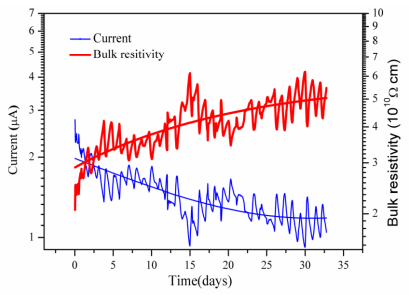
\includegraphics[width=0.80\textwidth]{GLA/resi.png}
	\captionof{figure}{Évolution du courant (courbe bleue) et de la résistivité volumique (courbe rouge) en fonction du temps d'une électrode de verre de basse résistivité soumise à une tension de \SI{1000}{\volt} pendant \num{32} jours.}
	\label{resi}
\end{figure}

La rugosité est excellente ce qui permet de n'appliquer aucun traitement de surface; contrairement aux RPC en bakélite. Ces traitements se sont révélés problématiques au cours des années \cite{1352718}.

L'inconvénient majeur de ce matériau est sa dimension maximale qui ne peut excéder \SI{32}{\centi\meter}$\times$\SI{30}{\centi\meter} (cf.fig~\ref{verre}). En effet, de par le procédé de fabrication (cf.fig~\ref{cooling}) de ces verres et par leur polissage à la main, de plus grandes dimensions sont irréalisables.
\marginpar
{
	\centering
	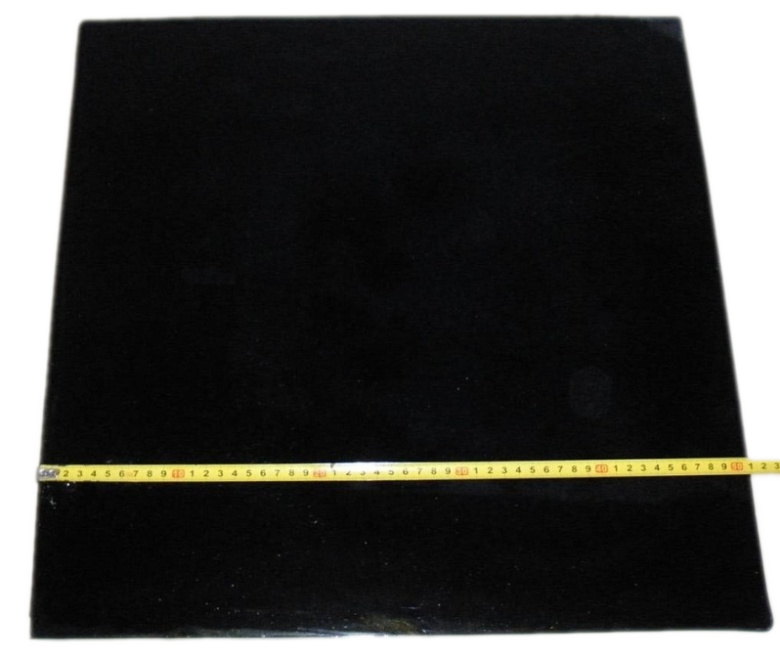
\includegraphics[width=\marginparwidth]{GLA/verre.png}
	\captionof{figure}{Photo d'une électrode de verre de basse résistivité.}
	\label{verre}
}
\marginpar
{
	\centering
	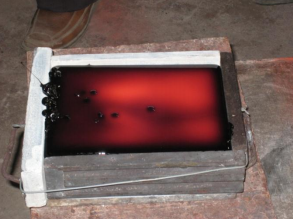
\includegraphics[width=\marginparwidth]{GLA/cooling.png}
	\captionof{figure}{Refroidissement d'un bloc de verre de basse résistivité.}
	\label{cooling}
}

Des détecteurs de cette dimension ont donc été construits afin d'étudier leurs caractéristiques et de voir s'ils étaient compatibles avec les demandes de CMS.

\section{Caractérisation des Glass Resitive Plate Chamber (GRPC)}
 
L'étude des GRPC passe par la connaissance de trois caractéristiques principales :
\begin{itemize}[label=$\bullet$]
	\item \textbf{L'Efficacité} de détection des particules. C'est la caractéristique principale. Elle est calculée en faisant le rapport entre le nombre de particules ayant été détectées et le nombre de particules ayant traversé le détecteur. Bien sûr, dans le cas où le signal est récolté par une électronique à seuil, la valeur de celui-ci va affecter l'efficacité de détection.
	\item \textbf{La multiplicité} représente le nombre de cellules ou bandes touchées lorsqu'une particule traverse le détecteur. En effet, plusieurs cellules de détection peuvent être déclenchées par le courant induit par les électrons créés lors de l'avalanche. Ici aussi le seuil appliqué à l'électronique influe sur la valeur de la multiplicité. La multiplicité joue un rôle très important sur la résolution spatiale du détecteur comme on le verra par la suite.
	\item \textbf{Le bruit électronique} qui est la fréquence de détection par l'électronique, d'un signal considéré comme non physique. Ceci peut être dû à une avalanche d'origine thermique ou radiative, par un courant dans la couche résistive etc. 
\end{itemize}

Un bon détecteur doit donc être proche d'une efficacité de 100\% avec une fréquence de bruit très basse. La multiplicité idéale dépend de la taille des cellules, du seuil appliqué et surtout de la résolution spatiale que l'on veut atteindre. D'autres caractéristiques du détecteur sont importantes telles que la sensibilité au bruit de fond (photons et neutrons par exemple) et l'évolution des caractéristiques du détecteur en fonction du temps, ce que l'on appelle le vieillissement du détecteur.

Ces détecteurs ont été instrumentés avec une électronique dite semi-digitale utilisée depuis de nombreuses années au laboratoire dans un prototype de calorimètre hadronique semi digital (SDHCAL) (cf.fig~\ref{SDHCAL}) \cite{Buridon:2016ill} pour le détecteur International Large Detector (ILD) (cf.fig~\ref{ILD}), l'un des deux détecteurs de l'expérience International Linear Collider (ILC) (cf.fig~\ref{ILC}).

\marginpar
{
	\centering
	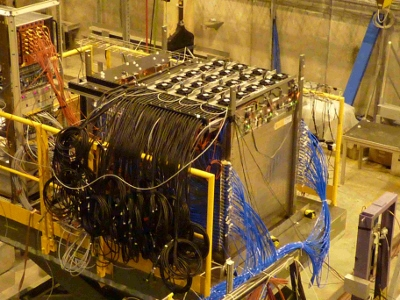
\includegraphics[width=\marginparwidth]{GLA/SDHCAL.jpg}
	\captionof{figure}{Photo du prototype SDHCAL construit à Lyon.}
	\label{SDHCAL}
}

\marginpar
{
	\centering
	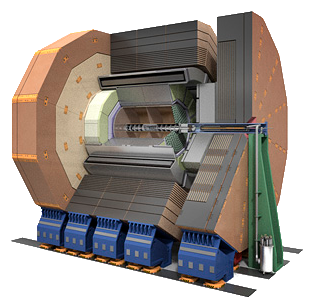
\includegraphics[width=\marginparwidth]{GLA/ILD.png}
	\captionof{figure}{Schéma de l'ILD.}
	\label{ILD}
}

\marginpar
{
	\centering
	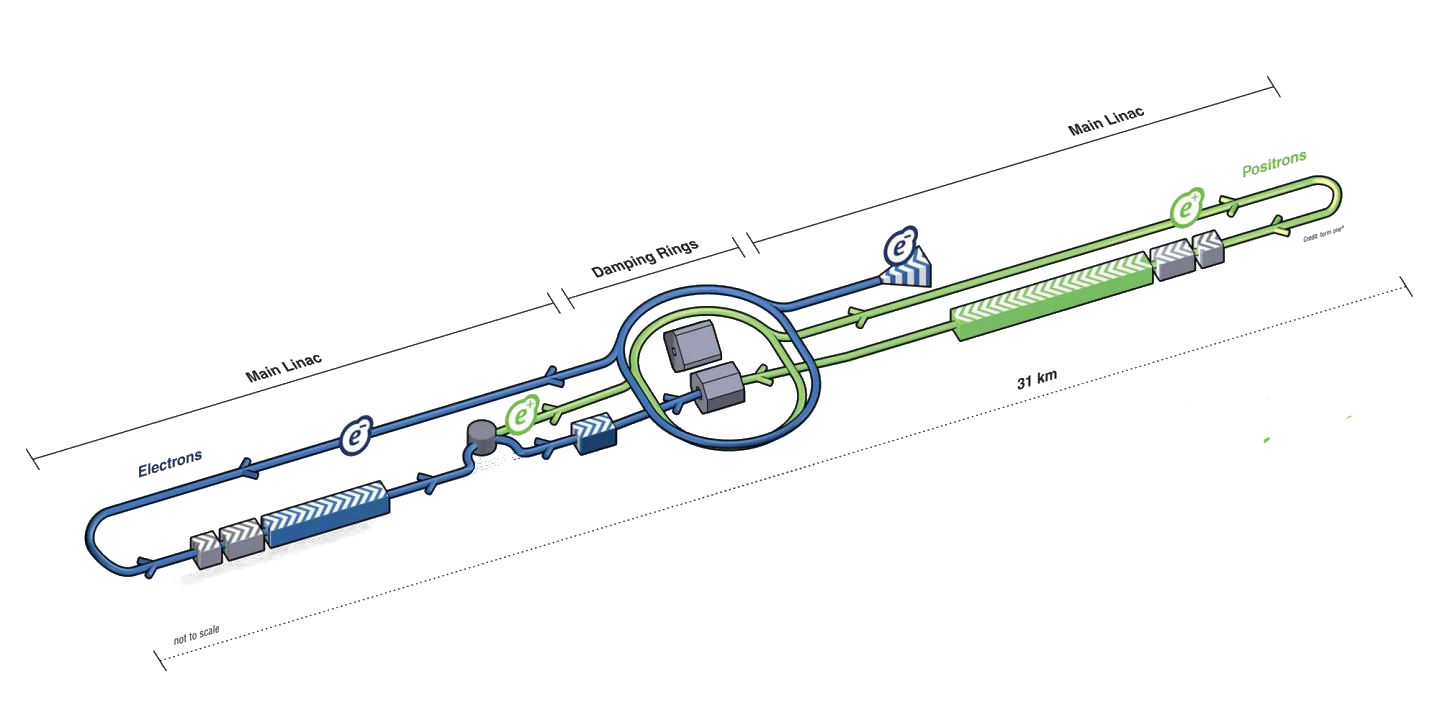
\includegraphics[width=\marginparwidth]{GLA/ILC.png}
	\captionof{figure}{Schéma de l'accélérateur ILC.}
	\label{ILC}
}

\section{Électronique "semi-digitale"}
Le SDHCAL est un prototype de calorimètre ultra-granulaire pour le \textit{Particle Flow Algorithm} (PFA). La taille des cellules de lecture de y est  \SI{1}{\square\centi\meter}. La balance entre la saturation de l'électronique et le volume de données à traiter à amener à opter pour une lecture à trois seuils (\num{2} bits). Pour ne pas introduire d'inhomogénéités, voire de zones mortes dues au système de refroidissement, il a été décidé de ne pas en utiliser. Pour cela, la puissance consommée par l'\textit{Application-specific integrated circuit} (ASIC) et donc la chaleur à dissipée sont réduites par l'emploi d'une alimentation intermittente dite pulsée, permettant de n'allumer l'ASIC que lorsque des données sont à enregistrer. Ce prototype utilise un type d'ASIC développé spécialement pour cette occasion, le HAdronic Rpc Detector ReadOut Chip (HARDROC)\cite{Dulucq:2010ssa}.

\subsection{La puce de lecture HARDROC}
L'ASIC HARDROC (cf.fig~ \ref{hardroc2},\ref{hardroc}) est issu d'une collaboration entre le pôle de microélectronique Omega d'Orsay et l'Institut de Physique Nucléaire de Lyon (IPNL). Cette puce est basée sur celle appelée OPERAROC qui est utilisée dans l'expérience OPERA).

\marginpar
{
	\centering
	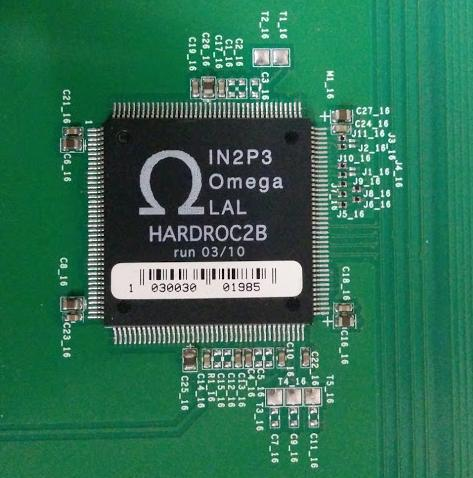
\includegraphics[width=\marginparwidth]{GLA/hardroc2.jpg}
	\captionof{figure}{Vue d'un HARDROC soudé.}
	\label{hardroc2}
}

\begin{figure}[ht!]
	\centering
	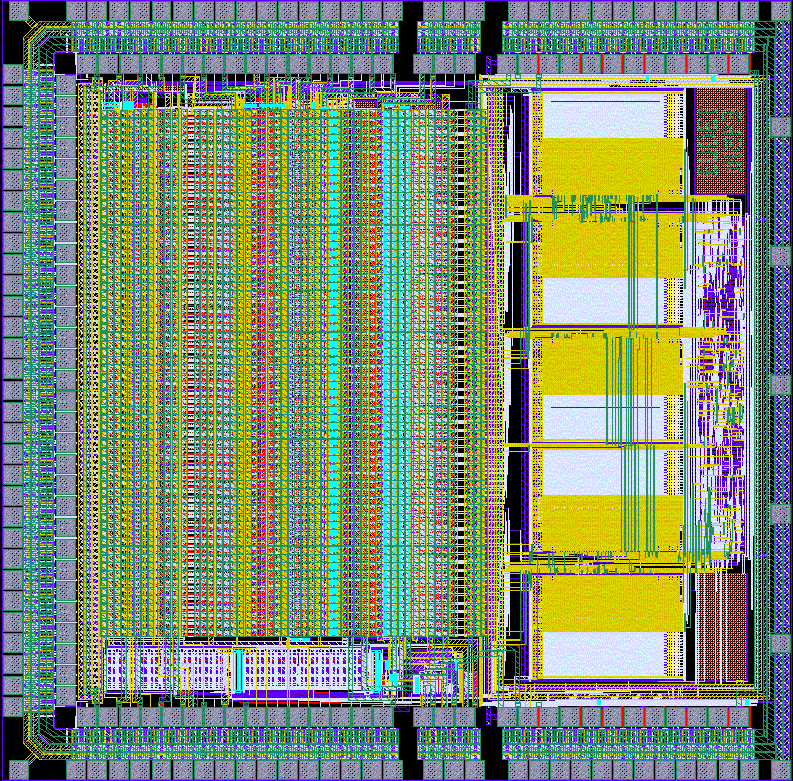
\includegraphics[width=0.35\textwidth]{GLA/HARDROC.png}
	\captionof{figure}{Schéma électronique du HARDROC.}
	\label{hardroc}
\end{figure}

Le HARDROC repose sur une technologie de fonderie AMS SiGe \SI{0.5}{\micro\meter}. La puce est ensuite insérée dans un boitier d'épaisseur \SI{1.4}{\milli\meter} qui comporte \num{160} pattes dont \num{64} voies. Les puces sont directement incorporées sur le Printed Circuit Board (PCB) du détecteur appellée Active Sensor Unit (ASU), chaque HARDROC étant connecté à \num{64} bandes ou carreaux de cuivre sensitifs (strip et pads respectivement) selon le PCB. Dans le cas des pads, la connection des pattes et des carreaux de cuivre est étudiée afin d'éviter la diaphonie entre les pattes.

Le schéma simplifié du HARDROC est donné par la figure \ref{scheme}. La partie digitale de la puce est commune aux \num{64} voies, alors que chacune possède sa partie analogique :

\begin{figure}[ht!]
	\centering
	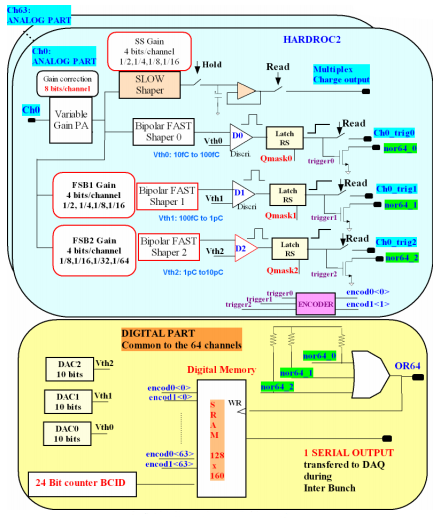
\includegraphics[width=0.65\textwidth]{GLA/scheme.png}
	\captionof{figure}{Schéma simplifié du HARDROC.}
	\label{scheme}
\end{figure}

Chaque voie d'entrée comporte :
\begin{itemize}[label=$\bullet$]
	\item Un préamplificateur de basse impédance fonctionnant en mode convoyeur de courant dont le gain est ajustable de \SIrange{0}{1.99}{}.
	\item Trois traitements de mise en forme rapide à gain réglable en parallèles \textit{Fast Shaper} (FSBs). Ils sont suivis d'un discriminateur de tension qui une fois déclenché, active une bascule (pour la sauvegarde de l'information).
	\item Un traitement de mise en forme lent \textit{Slow Shaper} qui permet le multiplexage du signal de sortie du préamplificateur et la lecture de la charge d'entrée. Ce traitement est surtout utilisé pour le débogage de la puce.
	\item Un encodeur pour coder le signal des bascules sur deux bits.
\end{itemize}

Les \num{3}$\times$\num{64} discriminateurs sont lus toutes les \SI{200}{\nano\second}. Les trois seuils des discriminateurs peuvent être ajustés grâce à trois convertisseurs digital-analogiques (DAC) codés sur \num{10} bits. Ce réglage affecte l'ensemble des \num{64} voies de la puce.

\subsubsection{Le préamplificateur}
L'entrée des cellules actives est reliée aux pattes "in\_pa" d'un préamplificateur de type "Super Base Commune" (cf.fig~\ref{preampli}), ce qui permet de diminuer l'impédance d'entrée (\SIrange{50}{100}{\ohm}) et donc d'éviter la diaphonie (\textit{cross-talk}). L'impédance d'entrée est donnée par la formule suivante :

\begin{equation}
Z_{in}=\frac{R_0+1/g_{m2}}{1+g_{m1}R_c}
\end{equation}
où $g_{m1}$ et $g_{m2}$ sont les transconductances des transistors $Q1$ et $Q2$.

\begin{figure}[th!]
	\centering
	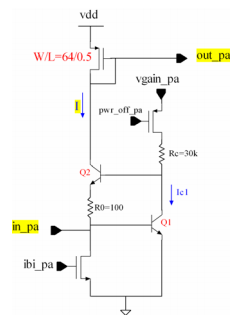
\includegraphics[width=0.60\textwidth]{GLA/preampli.png}
	\captionof{figure}{Schéma du préamplificateur.}
	\label{preampli}
\end{figure}

\subsubsection{Miroir de courant à 8 bits}
Le courant en sortie du préamplificateur est ensuite copié par huit miroirs de courant de gains respectifs 1/128, 1/64, 1/32, 1/16, 1/8, 1/4, 1/2 et 1 (cf.fig~ \ref{mirror}). La sortie est la somme des courants des miroirs activés. Les huit miroirs sont activables séparément grâce à un mot de \num{8} bits appelé contrôle de gain. La plage d'amplification varie donc de \SIrange{0}{1.992}{}. La précision de ce gain est estimée à 1.5\%. 

\begin{figure}[ht!]
	\centering
	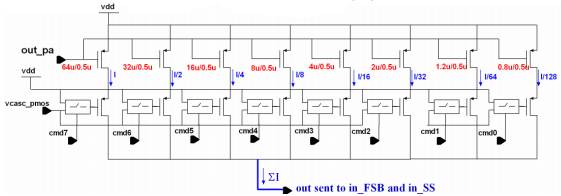
\includegraphics[width=0.8\textwidth]{GLA/miror.png}
	\captionof{figure}{Schéma du miroir de courant à \num{8} bits.}
	\label{mirror}
\end{figure}

\subsubsection{Les trois traitements de mise en forme rapide (FSB)}
En sortie du miroir à \num{8} bits, le signal passe dans trois circuits de traitement de mise en forme placés en parallèle. Ils consistent en un filtrage des signaux fournis en entrée afin d'éviter les perturbations dans le signal de sortie du préamplificateur ainsi que d'augmenter le rapport signal sur bruit. FSB1 et FSB2 (cf.fig~\ref{fsb1}) contrairement à FSB0 (cf.fig~\ref{fsb0}) possèdent un système de \num{4} miroirs de courant afin de réduire le gain en entrée et ainsi augmenter la gamme dynamique. Le filtre FSB0 est dédié aux charges d'entrée allant de \SI{10}{\femto\coulomb} à quelques centaines de \si{\femto\coulomb}, FSB1 qui possède \num{4} miroirs permet de traiter des signaux allant de \SI{100}{\femto\coulomb} à plus de \SI{1}{\pico\coulomb}; quant à FSB2 il permet de traiter des signaux de \SI{1}{\pico\coulomb} à \SI{30}{\pico\coulomb}.

\begin{figure}[ht!]
	\centering
	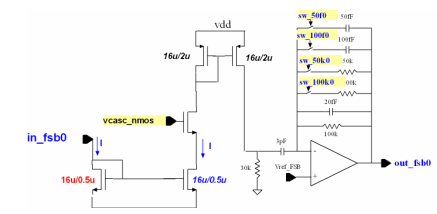
\includegraphics[width=0.60\textwidth]{GLA/FSB0.png}
	\captionof{figure}{Schéma de FSB0.}
	\label{fsb0}
\end{figure}

\begin{figure}[ht!]
	\centering
	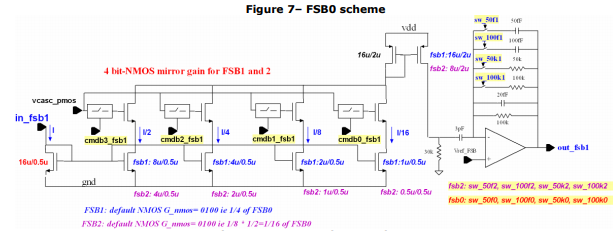
\includegraphics[width=0.8\textwidth]{GLA/FSB1.png}
	\captionof{figure}{Schéma de FSB1/2.}
	\label{fsb1}
\end{figure}

Il est possible d'activer des résistances et des condensateurs dans la boucle de contre réaction du filtre (cf.fig~\ref{fsb0},cf.fig\ref{fsb1}). Tout comme les gains des FSB, ils sont réglables par des mots binaires envoyés lors de la configuration des puces au début d'un run (slow control). Une étude poussée à été réalisée lors des tests pour le SDHCAL et nous avons gardé les valeurs trouvées comme les plus adaptées pour le gain des miroirs ainsi que pour la configuration de la boucle de contre-réaction.

La figure \ref{signal} montre la forme du signal en sortie des filtres FSB pour trois injections de charges différentes.
\begin{figure}[ht!]
	\centering
	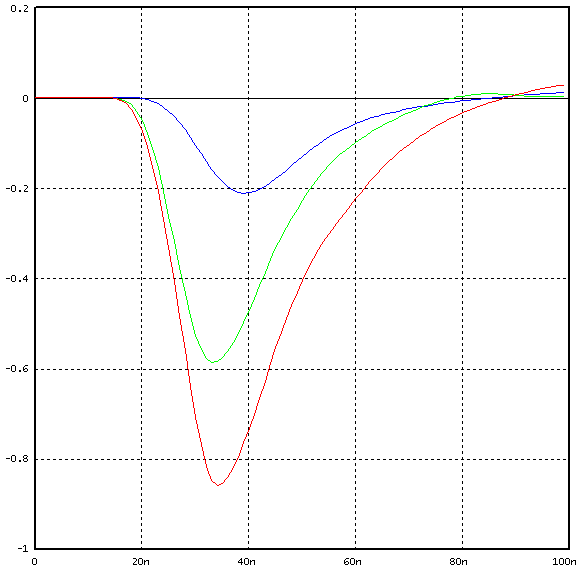
\includegraphics[width=0.45\textwidth]{GLA/SIGNAL.png}
	\captionof{figure}{Forme du signal en sortie des FSB pour des injections de charges de \SI{100}{\femto\coulomb} (bleu), \SI{1}{\pico\coulomb} (vert) et \SI{10}{\pico\coulomb} (rouge). FSB0 a pour gain \num{1}, FSB1 1/4 et FSB2 1/8.}
	\label{signal}
\end{figure}

\vspace*{-1.5cm}

\subsubsection{Discriminateurs et bascules}
Chaque sortie de FSB est connectée à un discriminateur. Les seuils des discriminateurs sont globaux aux \num{64} voies de la puce et sont réglables grâce à trois convertisseurs digital-analogique (DAC) de \num{10} bits (de \SIrange{0}{123}{}). Il est donc possible de régler le seuil de manière à déclencher le discriminateur pour une charge donnée déposée sur les cellules actives du détecteur.

Les facteurs de conversion, qui permettent de passer de la valeur du DAC à la valeur du seuil sur la charge induite sur une cellule active, ont été déterminés à l'aide d'injections de charges. Un condensateur de \SI{2}{\pico\farad} est activable par slow-control à cet effet, et permet d'injecter une charge donnée sur les \num{64} canaux du HARDROC. Pour chaque valeur de charge injectée, la valeur du seuil de basculement correspondant à une efficacité de détection de 50\% a été mesurée \cite{kieffer:tel-00751999}. Les courbes de ces valeurs de basculement pour chaque canal en fonction de la charge injectée sont ensuite obtenues, pour chaque seuil. En soustrayant les piédestaux ont obtient les courbes de la figure \ref{seuils}.

\begin{figure}[ht!]
	\centering
	\subfloat[Seuil de basculement pour DAC0]{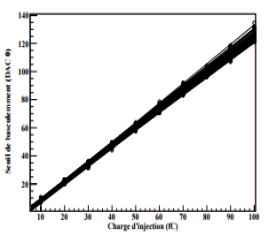
\includegraphics[width=.30\linewidth]{GLA/seuil1.png}}
	\hfill
	\subfloat[Seuil de basculement pour DAC1]{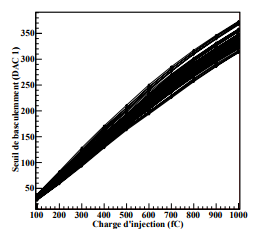
\includegraphics[width=.30\linewidth]{GLA/seuil2.png}}
	\hfill
	\subfloat[Seuil de basculement pour DAC2]{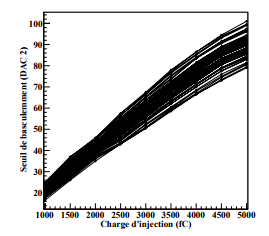
\includegraphics[width=.30\linewidth]{GLA/seuil3.png}}
	\caption{Seuil de basculement pour seuils (DAC0, DAC1, DAC2), en fonction de la charge injectée, pour \num{64} canaux d'un HARDROC. La valeur du piédestal a été soustraite.}
	\label{seuils}
\end{figure}%

L'ajustement linéaire des courbes \ref{seuils} permet d'obtenir la valeur du seuil en fonction de la valeur de DAC pour chaque seuil :

\begin{equation}
\mbox{Seuil}_{i}=\frac{\mbox{DAC}_{i}-p_{i}}{\lambda_{i}} [pC]
\label{equationn}
\end{equation}

où $\lambda_{i}$ est le coefficient directeur de la droite obtenue après ajustement linéaire et $p_{i}$ est la valeur du piédestal. Les valeurs de ces paramètres pour chaque seuil sont données dans le tableaux suivant :

\begin{table}[H]
	\centering
\begin{tabular}{|O|O|O|N}
	\hline 
	Seuil & $\lambda$ & Piédestal \\ 
	\hline 
	\num{0}&\num{700} &\num{90} \\ 
	\hline 
	\num{1}& \num{80} & \num{98} \\ 
	\hline 
	\num{2}&\num{16.3} &\num{98} \\ 
	\hline 
\end{tabular} 
	\captionof{table}{Valeur des paramètres $\lambda$ et piédestaux pour les trois seuils.}
\end{table}

Les courbes \ref{seuils} n'étant pas linéaires sur toute la plage, nous avons veillé à ne pas dépasser la zone non linéaire lors de nos tests en faisceaux.

Chaque discriminateur est relié à une bascule de type RS qui, dès lors que le discriminateur correspondant est déclenché et le signal autorisant l'acquisiton est à l'état haut, passe à l'état haut. Lors du coup d'horloge suivant, toutes les \SI{200}{\nano\second}, les bascules sont lues et remises à zéro. Les trois valeurs des bascules correspondant à une cellule active sont ensuite envoyées dans un encodeur qui code ces informations sur deux bits selon le tableau \ref{encodage}.

\begin{table}[H]
	\centering
	\begin{tabular}{|O|O|O|O|N}
		\hline 
		Seuil0  & Seuil1 & Seuil2 &Sortie \\ 
		\hline 
		\num{0}  & \num{0} & \num{0} & $00_{2}$ \\ 
		\hline 
		\num{1}  & \num{0} & \num{0} & $10_{2}$ \\
		\hline 
		\num{1} & \num{1} & \num{0} &  $01_{2}$ \\
		\hline
		\num{1}  & \num{1} & \num{1} & $11_{2}$ \\
		\hline
	\end{tabular} 
	\captionof{table}{Encodage des seuils sur \num{2} bits.}
	\label{encodage}
\end{table}

Il est également possible de masquer une cellule active bruyante en configurant la puce de telle manière que la bascule soit à l'état bas en permanence. Ce réglage peut se faire grâce à des bits de masque envoyés lors du slow control.

\subsubsection{Le registre de contrôle lent (slow control)}
Afin de configurer le HARDROC, une patte d'entrée est utilisée. Une ligne d'horloge est mise en marche et à chaque front montant, les informations sont propagées dans le registre à décalage présent dans le HARDROC. \num{872} fronts d'horloge sont nécessaires afin de régler le HARDROC (valeurs des seuils, gain des préamplificateurs, gains des FSB, masques etc...). Une fois toutes les informations envoyées, il suffit d'arrêter l'horloge. La dernière bascule du registre est connectée à une patte qui permet à la fois de chainer les HARDROC et ainsi les configurer en série, mais aussi de vérifier que les bascules sont dans le bon état. Pour cela il suffit de redémarrer l'horloge et de comparer le mot binaire récupéré en sortie et le mot envoyé en entrée.

\subsubsection{La mémoire du HARDROC}
À chaque coup d'horloge, lorsque la puce est en phase d'acquisition, un OU logique est réalisé entre les bascules des \num{64} voies de la puce. Si l'une d'elle est à l'état haut, la mémoire digitale (Digital Memory) (cf.fig~\ref{scheme}) reçoit un signal pour enregistrer l'événement. La valeur de l'horloge de l'événement, appelée Bunch Crossing ID (BCID) ainsi que le numéro d'identification de l'ASIC ainsi que la valeur de tous les encodeurs de la puce seront enregistrés. 

La mémoire du HARDROC permet de stocker \num{128} événements de \num{160} bits (cf.tab~\ref{bits}). Une fois sa mémoire pleine, un signal de saturation est émis sur une patte dédiée.

\begin{table}[H]
	\centering
	\begin{tabular}{|O|O|N}
		\hline 
		Contenu d'un événement (valeur autorisée) & Taille (octets) \\ 
		\hline 
		Header : Identifiant de l'ASIC (\SIrange{0}{255}{})  & \num{1} \\ 
		\hline 
		BCID : Compteur d'horloge (\SIrange{0}{16777215}{}) & \num{3}\\
		\hline 
		États des canaux \SIrange{48}{63}{}  & \num{4} \\
		\hline
		États des canaux \SIrange{32}{47}{}  & \num{4} \\
		\hline
		États des canaux \SIrange{16}{31}{}  & \num{4} \\
		\hline
		États des canaux \SIrange{0}{15}{}  & \num{4} \\
		\hline
	\end{tabular} 
	\captionof{table}{Contenu d'un événement de HARDROC et taille en octets.}
	\label{bits}
\end{table}
 
\subsection{L'acquisition des données}
Le HARDROC à été conçu pour être chaîné, afin de piloter de nombreuses puces avec un nombre réduit de lignes communes. L'exemple du slow control montre l'intérêt de ce chainage. Afin de gérer plusieurs HARDROC, une carte électronique composée d'un Field-Programmable Gate Array (FPGA), appellée Detector InterFace (DIF) (cf.fig~\ref{DIF}) a été développée en collaboration avec le Laboratoire d'Annecy de Physique des Particules (LAPP). Cette carte possède un controleur USB utilisé pour le rapatriement des données et l'envoi des informations du slow control, d'un port HDMI dont un protocole développé pour l'occasion permet la synchronisation des horloges et de connecter la DIF à une carte de contrôle. Elle dispose également de plusieurs entrées/sorties LEMO qui peuvent être utilisées entre autres pour injecter un signal de déclenchement externe ou que de remonter un signal "busy".

\begin{figure}[ht!]
	\centering
	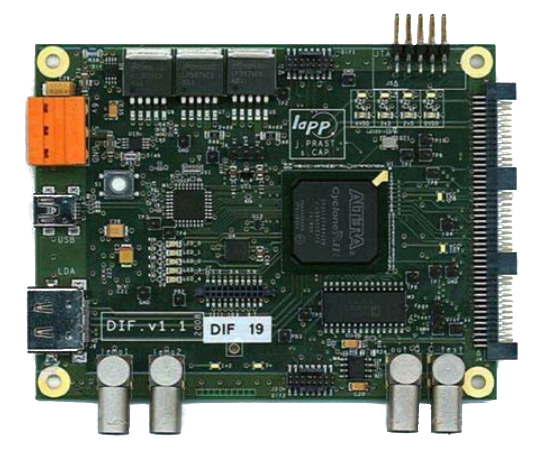
\includegraphics[width=0.55\textwidth]{GLA/DIF.png}
	\captionof{figure}{Photo d'une DIF.}
	\label{DIF}
\end{figure}

Pour commencer l'aquisition, la DIF envoie à tous les HARDROC un signal dit d'événement valide. Ceci à pour effet de remettre à zéro leur compteur interne (BCID). Chaque événement correspondant à une cellule activée touchée est ensuite enregistré dans la mémoire du HARDROC connécté à cette cellule. Lorsqu'un HARDROC a sa mémoire pleine, un signal de saturation est envoyé à la DIF par une ligne commune. On procède alors à la lecture des mémoires des HARDROC (ReadOut). Chaque ASIC envoie le contenu de sa mémoire sur une ligne commune appelé ligne de données. Une ligne (Transmission ON) permet de prévenir la DIF qu'un des HARDROC procède au transfert de ses données. Le fait de transférer les données en série amène à un temps mort maximum de

\begin{equation}
n\times(128 \times 160)\si{\bits}\times \SI{200}{\nano\second}= n*\SI{4.09}{\milli\second}
\end{equation} 

où $n$ est le nombre de HARDROC. Une fois tous les événements récoltés, les mémoires sont remises à zéro. Le diagramme temporel \ref{temp} résume le cycle d'acquisition et de lecture décrit ci-dessus.

\begin{figure}[ht!]
	\centering
	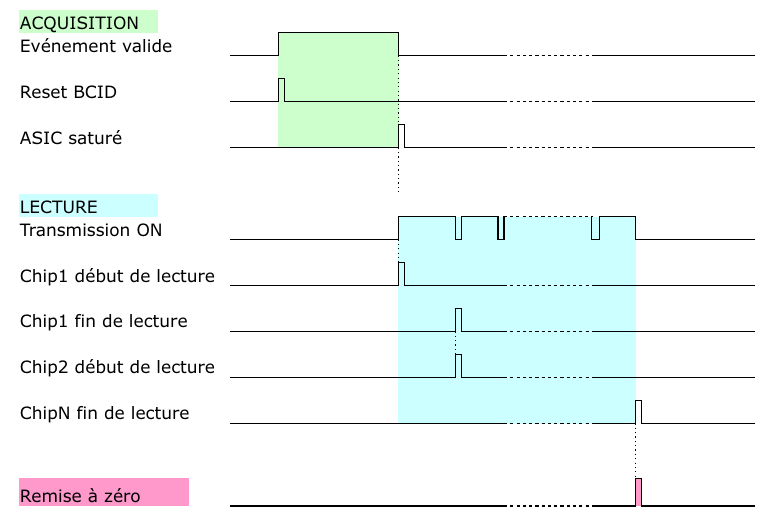
\includegraphics[width=0.48\textwidth]{GLA/cycle.png}
	\captionof{figure}{Diagramme temporel du cycle d'acquisition et de lecture.}
	\label{temp}
\end{figure}

Afin de faciliter la reconstruction et l'analyse des données, des informations additionnelles sont ajoutées au flux de données des HARDROC par la DIF. À chaque ReadOut, les données des ASICS sont encapsulées par un header et un trailer ainsi que d'autres informations telles que des compteurs. Ces DIF sont reliées par l'intermédiaire de câbles HDMI à une Synchronous Data Concentrator Card\footnote{Le nombre de chambres testées a toujours été inférieur à \num{9} ce qui permet de se passer de DCC et de connecter directement les DIF des chambres à la SDCC.} (SDCC) (cf.fig~\ref{SDCC}) \cite{Baulieu:2015pfa} qui reçoit les busy et les RAMfull des DIF et envoie de manière synchrone l'horloge et les commandes. La carte SDCC est directement reliée par USB à l'ordinateur controllant la DAQ.

\marginpar
{
	\centering
	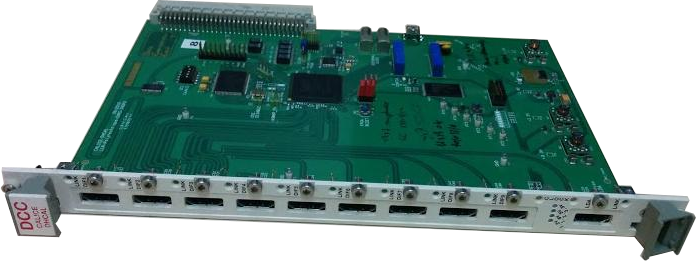
\includegraphics[width=\marginparwidth]{GLA/SDCC.png}
	\captionof{figure}{Une (S)DCC.}
	\label{SDCC}
}


La chaine d'acquisition peu être résumée par le schéma \ref{chaine}. 

\begin{figure}[ht!]
	\centering
	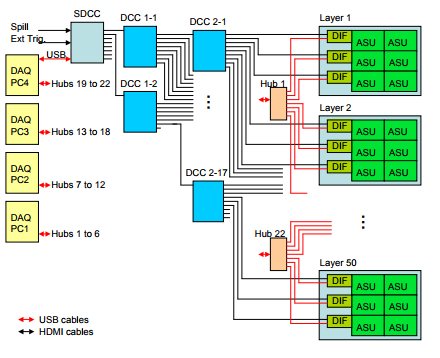
\includegraphics[width=0.48\textwidth]{GLA/chaine.png}
	\captionof{figure}{Architecture de la DAQ du SDHCAL. Dans notre cas le nombre d'ASU est d'un par layer (chambre) ainsi que d'une DIF par chambre. Le nombre de chambres étant dans notre cas inférieur à \num{9}, l'utilisation des DCC est inutile.}
	\label{chaine}
\end{figure}

\subsection{Format de données LCIO}
La chaine d'acquisition et l'électronique ayant été conçues pour le détecteur ILD de ILC, les données sont sauvegardées dans le format de données Linear Collider I/O (LCIO)\cite{2003physics6114G}. Ce format repose sur un modèle d'événement générique  dans lequel les données sont organisées en collections. Chaque collection contient une liste d'objets dont la structure est adaptée à l'information à stocker ainsi qu'une liste de paramètres. À chaque début d'acquisiton un fichier LCIO est créé et les événements sont stockés dans un LCEvent contenant une collection d'objets de type LCGenericObject ("RU XDAQ") qui contiennent les données brutes de chaque DIF enregistrées sous forme d'entiers.

Ces fichiers peuvent ensuite être lus et analysés en créant des algorithmes qui sont implémentés sous forme de processeurs codés en \Cpp et utilisés par le framework Modular Analysis \& Reconstruction for the LINear collider (MARLIN) \cite{Gaede:2006pj}. Chaque processeur analyse les données dans les LCEvent et peut créer de nouvelles collections qui sont ajoutées à l'événement ou sont insérées dans les LCEvent d'un nouveau fichier. MARLIN permet de définir les processeurs et l'ordre dans lequel les lancer à l'éxécution sans recompilation. Pour cela il utilise un fichier Extensible Markup Language (XML) de configuration appelé "steering file". Il est également possible de définir dans ce fichier les paramètres nécessaires aux processeurs.

\section{Programme d'analyse pour les chambres à élecronique HARDROC}
L'un des travaux de notre thèse a été de se familiariser avec ce framework et de programmer des processeurs afin d'analyser les données en provenance des détecteurs. 

\subsection{Les processeurs MARLIN}
Trois processeurs permettent de structurer les données afin d'en tirer les caractéristiques des détecteurs présentées précédemment :

\begin{itemize}[label=$\bullet$]
	\item Le processeur Streamout permet de mettre en forme les données brutes et de passer des LCGenericObject en une collection de RawColorimeterHit qui correspondent à des cellules touchées. Ces objets contiennent le numéro de la voie touchée du HARDROC (Channel\_Id), le numéro de l'HARDROC touché (ASIC\_Id) ainsi que le numéro de la DIF s'occupant de cet HARDROC (DIF\_Id).
	\item Le processeur Trivent permet de passer du triplet (Channel\_Id,ASIC\_Id,DIF\_Id) à la position locale dans la chambre ($I$,$J$,$K$=numéro de la chambre). La position des chambres (DIF) dans l'espace est contenue dans un fichier XML qui est un paramètre du steering file de MARLIN, ce qui permet le passage des positions locales dans une chambre aux positions réelles ($X$,$Y$,$Z$) dans l'espace, de la cellule touchée. Trivent permet aussi de présélectionner les candidats muons. En effet, les données récoltées correspondent à tous les hits collectés jusqu'à ce qu'un HARDROC soit plein. Les données collectées inclues non seulement des hits venant de muons mais aussi des hits de bruits etc. Pour sélectionner les candidats muons, une agrégation en temps est réalisée. Les coups d'horloge (BCID) qui présentent plus de $N_{hit}=3$ hits sont sélectionnés. Pour chaque coup d'horloge sélectionné, les hits appartenant à des coups d'horloge contenus dans une fenêtre de $\pm t_{fen}=\pm3$ sont combinés pour construire un candidat muon. Si deux candidats sont proches et leur fenêtres se chevauchent, ils ne sont pas pris en compte afin de ne pas ajouter plusieurs fois les hits dans plusieurs candidats muons. Tous les hits sélectionnés pour un même candidat muon appartiennent à une même collection et à un même événement.
	\item Le processeur Analysis utilise ces candidats muons et effectue une sélection plus fine des candidats muons. Premièrement les évènements contenant un trop gros nombre de hits dans une chambre sont rejectés. Afin d'estimer l'éfficacité d'une chambre, les barycentres des hits des autres chambres sont utilisés afin de créer un candidat trace. Pour cela une minimisation par $\chi^2$ est utilisée. Les $\chi^2$ sont donnés par :
	
	\begin{equation}
	\chi_{xz}^2=\sum_i^{N_{chambre-1}}\left(x(z_{i})-x(z_{i})_{ba}\right)^2 \quad \chi_{yz}^2=\sum_i^{N_{chambre-1}}\left(y(z_{i})-y(z_{i})_{ba}\right)^2
	\end{equation}
	
	où $x(z_{i})_{ba}$ et $y(z_{i})_{ba}$ sont les coordonnées du barycentre des hits dans la chambre $i$ et :
	
\begin{equation}
\begin{cases}
\strut x(z_i)=az_i+b\\
y(z_i)=cz_i+d
\end{cases}
\end{equation}

est l'équation paramétrique d'une droite dans l'espace avec \num{4} paramètres $a,b,c,d$. La minimisation est effectuée grâce au paquet MINUIT \cite{James:2004xla} contenu dans le framework ROOT \cite{BRUN199781}.
Si la droite traverse la chambre étudiée et si des hits sont situés dans une région de $\pm 3$ cellules $\times\pm 3$ cellules, ou $\pm 3$ strips du point d'impact, la chambre est considérée efficace pour cet événement. Le nombre de hits dans cette région est utilisé comme estimateur de la multiplicité du détecteur.
\end{itemize}

Le fait d'avoir conçu les processeurs de telle manière que la géométrie ne soit connue que dans un fichier XML possède de nombreux avantages. Cela permet notamment de pouvoir changer facilement une DIF ou une chambre du détecteur sans avoir à recompiler les processeurs, de garder une trace des géométries utilisées sous forme lisible et claire. Cela à également permis de faire fonctionner ces processeurs sur une simulation du prototype du SDHCAL afin de vérifier que ces processeurs donnaient la bonne efficacité alors que ni le nombre de chambres (48 pour le SDHCAL), ni le nombre d'ASU et de DIF par chambre (6 et 3 respectivement) ne sont identiques à nos détecteurs placés en tests en faisceaux.

\subsubsection{Test des processeurs par une simulation du SDHCAL}
Le test des processeurs utilise une simulation du SDHCAL basée sur GEANT4\cite{AGOSTINELLI2003250} qui simule la propagation des particules dans le détecteur. Le champ électrique entre les deux électrodes de verre des GRPC n'est pas simulé. En revanche, les avalanches sont modélisées par un algorithme appellé SimDigital qui est en fait un processeur MARLIN disponible dans le paquet MarlinReco \cite{2007Prama} de ILCSoft. Cet algorithme s'occupe également de la répartition de la charge sur les carreaux de cuivre. Une description détaillée de cet algorithme ainsi que de son paramétrage est donnée dans \cite{steen:tel-01282680}.

L'algorithme utilise les segments de GEANT4 créés par les particules incidentes chargées. Il arrive cependant, que plusieurs segments soient créés par GEANT4 pour une même particule incidente dans la même couche de gaz. Ces segments pourraient chacun produire une avalanche. Afin d'éviter que cela n'arrive, les segments sont reliés entre eux pour ne former qu'un segment.

 À chaque volume de gaz correspondant à une cellule de lecture $C_{0}$, la longueur des segments contenus dans ce volume est calculé. Les segments de taille inférieure à \SI{1}{\micro\meter} sont supprimés.
 
 Une carte d'efficacité pour chaque ASIC est ensuite appliquée afin de tenir compte des gaz \chemform{CO_2} et \chemform{SF_6} dont les effets ne sont pas pris en charge par GEANT4. Il est aussi possible de forcer les efficacités d'une chambre par ces cartes. Une chambre possédant une carte d'efficacité de 50\% aura donc une probabilité de 50\% que les segments passant par sa couche de gaz soient conservés.
 
 La charge induite par chaque segment est ensuite aléatoirement choisie en utilisant une distribution de Polya:
 
 \begin{equation}
 P(q)=\left[\frac{q}{\bar{q}}(1+\theta)\right]^\theta\exp^{-\left[\frac{q}{\bar{q}}(1+\theta)\right]}
 \end{equation}
 
 où $\bar{q}$ est la valeur moyenne en \si{\pico\coulomb} et $\theta$ un paramètre libre lié à la largeur de la distribution. Afin de tenir compte de l'angle d'incidence, la charge induite est corrigée $Q_{corr}$.
 
 Lorsque deux avalanches sont très proches l'une de l'autre et se chevauchent, le signal induit n'est pas la somme des signaux de chaque avalanche. Pour simuler cet effet, lorsque deux segments sont situés à une distance inférieure à une valeur $d_{cut}$, seul le segment dont la charge induite est la plus élevée est gardé.
 
 La charge induite est ensuite répartie sur la cellule $C_0$ et sur les cellules voisines se trouvant à une distance inférieur à $r_{max}$ de $C_0$. Un rapport est alors calculé pour chaque cellule :
 
 \begin{equation}
 R_i=\frac{\int_{a_i}^{b_i}\int_{c_i}^{d_i}\sum_{j=0}^{n-1}\alpha_j\exp^{\frac{(x-x_0)^2+(y-y_0)^2}{2\sigma_j^2}}\dd x\dd y}{\int_{-r_{max}}^{+r_{max}}\int_{-r_{max}}^{+r_{max}}\sum_{j=0}^{n-1}\alpha_j\exp^{\frac{(x-x_0)^2+(y-y_0)^2}{2\sigma_j^2}}\dd x\dd y}
 \end{equation}
 
où $a_i$, $b_i$, $c_i$ et $d_i$ sont les positions des bords de la cellule $i$, $(x_0,y_0)$ sont les coordonnées du milieu du segment, $n$, $\alpha_j$ et $\sigma_j^2$ sont des paramètres libres. Ainsi $C_0$ est ses voisins se voient ajouter une charge induite de $R_iQ_{corr}$.

Pour finir les seuils des cellules sont appliqués. Seules les cellules possédant une charge supérieure au seuil seront considérées comme étant touchées et créeront un hit.

Nous avons utilisé cette simulation en simulant le passage de muons de \SI{100}{\giga\eV} dans le prototype SDHCAL dont les cartes d'efficacités des \num{48} chambres ont été fixées successivement de 10\% à 100\% par pas de 10\%. La figure \ref{effisimul} montre les efficacités calculées par le processeur Analysis pour les \num{48} chambres du SDHCAL et les \num{10} cartes d'efficacité.

\begin{figure}[ht!]
	\centering
	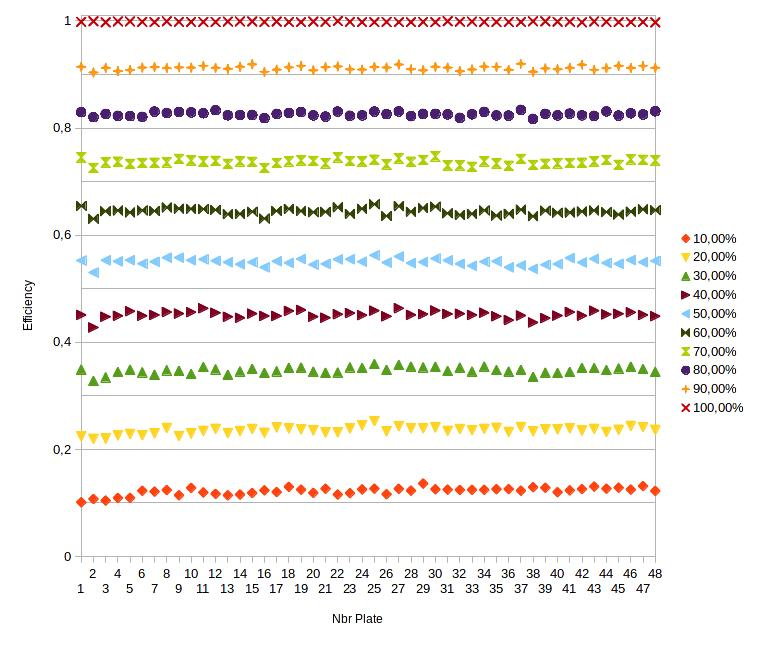
\includegraphics[width=0.62\textwidth]{GLA/effisimul.jpg}
	\captionof{figure}{Efficacité trouvée par le processeur Analysis pour les \num{48} chambres du SDHCAL en utilisant la simulation SimDigital. Les particules incidentes sont des muons de \SI{100}{\giga\eV} et chaque couleur représente une carte d'efficacité fixée lors de la simulation.}
	\label{effisimul}
\end{figure}

Cette figure montre bien que l'on arrive a retrouver l'efficacité fixée dans les cartes d'efficacités de la simulation. Une divergence semble apparaitre et augmenter jusqu'à 50\% puis diminuer. Elle est au maximum de 5\%. Elle peut s'expliquer par le fait qu'une fraction des muons produit plus d'un segment dans la couche de gaz d'une chambre. En faisant l'hypothèse que seul un ou deux segments peuvent être créés par un muon et en notant $f$ la fraction de muons donnant lieu à deux segments dans la couche de gaz et $\epsilon$ la probabilité de garder un segment dans la simulation, l'inefficacité de la chambre vaut :

\begin{equation}
(1-f)(1-\epsilon)+f(1-\epsilon)^2=1-(f+1)\epsilon+f\epsilon^2 \label{equa1}
\end{equation}

En prenant le cas des cartes d'efficacités 50\%, l'inefficacité de la chambre est d'environ 45\%. Ce qui permet d'estimer le coefficient $f$ à $0.2$. La figure \ref{plotvaleur} donne le graphe de la fonction \ref{equa1} pour $f=0.2$. Le tableau \ref{tableauvaleur} donne les valeurs attendues de l'efficacité des chambres pour les valeurs des cartes d'efficacités utilisées pour la construction de la figure \ref{effisimul}. On remarque que les valeurs calculées par la formule \ref{equa1} sont très proches des valeurs calculées par les processeurs MARLIN.
\vspace*{-0.6cm}
	\begin{figure}[ht!]
    \subfloat[Graphique des valeurs de l'efficacité attendue pour différentes valeurs de la carte d'efficacités.]{\label{plotvaleur}\raisebox{-.5\height}{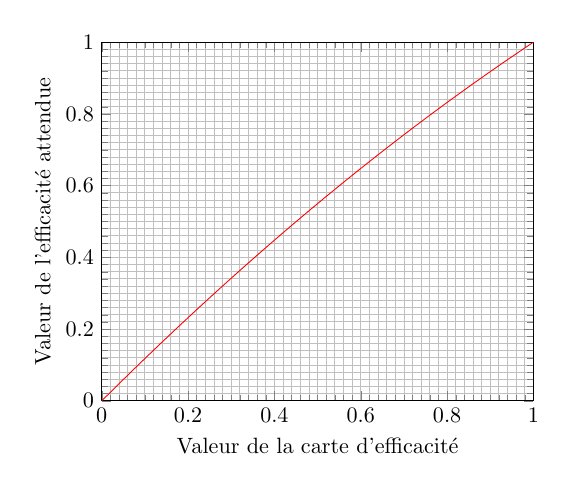
\begin{tikzpicture}[scale=0.80]\begin{axis}[grid=both,xlabel={Valeur de la carte d'efficacité},ylabel={Valeur de l'efficacité attendue},minor tick num=9,xmin=0,xmax=1.0,ymin=0,ymax=1.0]\addplot[mark=none,domain=0:1.0,samples=30,color=red]{1-((1-x)*(1-0.2*x))};\end{axis}\end{tikzpicture}}}
    \hfill
	\subfloat[Tableau des valeurs de l'efficacité attendue pour différentes valeurs de la carte d'efficacités.]{\label{tableauvaleur}\hfill\begin{tabular}{|O|O|N}
			\hline
            Carte d'efficacités & Valeur attendue \\
			\hline 
			10\% & 11,80\% \\ 
			\hline 
			20\% & 23,20\% \\ 
			\hline 
			30\% & 34,20\% \\ 
			\hline 
			40\% & 44,80\% \\ 
			\hline 
			50\% & 55,00\% \\ 
			\hline 
			60\% & 64,80\% \\ 
			\hline 
			70\% & 74,20\% \\ 
			\hline 
			80\% & 83,20\% \\ 
			\hline 
			90\% & 91,80\% \\ 
			\hline 
		\end{tabular}\hfill}
	\caption{Comparaison entre la valeur attendue et la valeur mise dans la carte d'efficacité avec $f=0.2$. }
	\label{Comparaison}
\end{figure}

\vspace*{-0.8cm}
 Tous les résultats à partir de juin 2015 présentés dans cette thèse qui ont rapport avec des chambres instrumentées avec des HARDROC ont été réalisés avec ces processeurs.
\vspace*{-0.3cm}
\section{Tests en faisceaux}
\vspace*{-0.3cm}
De nombreux tests en faisceaux ont été réalisés lors de cette thèse, notamment afin de vérifier et de compléter les résultats obtenus lors d'un test en faisceaux à DESY en Allemagne en Janvier 2012.
\vspace*{-0.25cm}
\subsection{Tests en faisceaux à DESY}
\vspace*{-0.25cm}
Un test en faisceaux à DESY \cite{Haddad:2012fx} a été réalisé afin de vérifier les caractéristiques des verres de basse résistivité produits par l'université de Tsinghua. Des chambres en verre de basse résistivité de $30\times30$\si{\square\centi\meter} (GRPC) (cf.fig~\ref{chambre}) instrumentée par une électronique composée de HARDROC et de cellules de lecture en forme de pads (cf.fig~\ref{cellule}) ont été soumises à un faisceau intense et continu d'électrons d'énergie allant jusqu'à \SI{6}{\giga\eV} couvrant une surface de quelques \si{\square\centi\meter}. L'épaisseur des électrodes est de \SI{1}{\milli\meter} et celle du gap est de \SI{1.2}{\milli\meter}. Le flux d'électrons est au maximum de \SI{35}{\kilo\hertz}. Le mélange de gaz est composé de 93\% de \chemform{TFE}(\chemform{C_2F_4}), 5\% de \chemform{CO_2} et 2\% de \chemform{SF_6} (mélange ILC).

\noindent
\begin{minipage}[th!]{.48\textwidth}
\centering
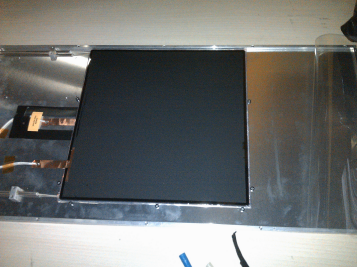
\includegraphics[width=0.68\textwidth]{GLA/chambre.png}
\captionof{figure}{Une GRPC composée de verre de basse résistivité ($\sim 10^{10}$\si{\ohm.\cm}).}
\label{chambre}
\end{minipage}%
\hfill
\begin{minipage}[th!]{.48\textwidth}
	\centering
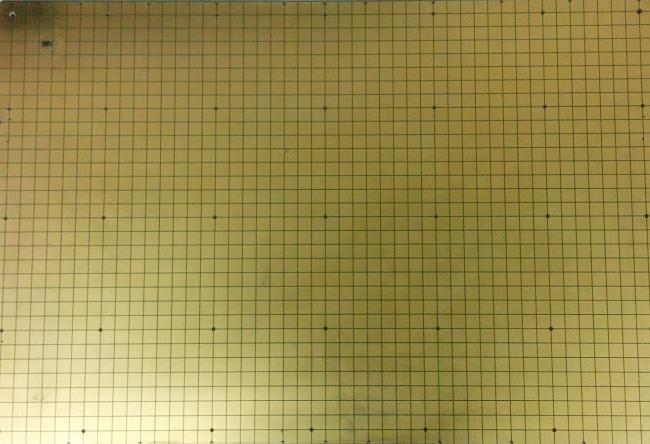
\includegraphics[width=0.65\textwidth]{GLA/cellules.jpg}
\captionof{figure}{Cellules de lecture de taille \SI{1}{\centi\meter}$\times$\SI{1}{\centi\meter}.}
\label{cellule}
\end{minipage}

Ce test en faisceau a montré que les verres de basse résistivité peuvent supporter un flux de particules de \SI{9}{\kilo\hertz\per\square\centi\meter} tout en gardant une efficacité proche de 90\% (cf.fig~\ref{effiDesy}). Le point de fonctionnement a été estimé à \SI{7.2}{\kilo\volt} donnant une efficacité de 95\% et une multiplicité de $1.4$, pour un seuil de \SI{50}{\femto\coulomb}. 

\begin{figure}[ht!]
	\centering
	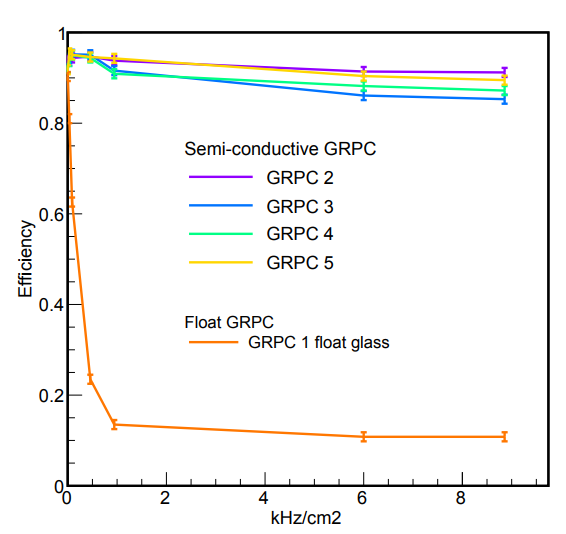
\includegraphics[width=0.7\textwidth]{GLA/effiDesy.png}
	\captionof{figure}{Efficacité en fonction du flux de particules pour différentes GRPC. La ligne orange correspond à une chambre composée de verre "Standard" dit \textit{Float Glass} de resistivité de l'ordre de $\sim10^{13}$\si{\ohm.\cm}. Les autres courbes correspondent à des chambres composées de verre de basse résistivité.}
	\label{effiDesy}
\end{figure}

Alors que dès \SI{1}{\kilo\hertz\per\square\centi\meter}, les chambres de verre standard voient leur efficacité chuter autour de 20\%, les chambres construites avec des électrodes en verre de basse résistivité continuent à être efficaces même après \SI{9}{\kilo\hertz\per\square\centi\meter}. Leur efficacité décroit très lentement en fonction du flux de particules.

\subsection{Tests en faisceaux au PS}
Huit chambres GRPC ont été amenées au PS (cf.fig~\ref{complexe}) en Juin \num{2014} dans la Zone Est (ligne de faisceau T9), juste avant le début de cette thèse, afin de former un télescope (cf.fig~\ref{TelescopePS}).

\begin{figure}[ht!]
	\centering
	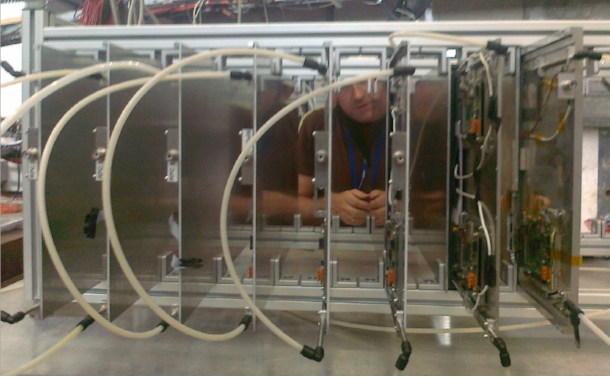
\includegraphics[width=0.50\textwidth]{GLA/TelescopePS.png}
	\captionof{figure}{Télescope utilisé pour le test en faisceaux au PS. La chambre à strips est placée en deuxième position en partant de la droite.}
	\label{TelescopePS}
\end{figure}

Une chambre possède une électronique à strips et les sept autres une électronique à pads. La chambre à strips est de type "double gap" (cf.fig~\ref{DoubleGap}) : deux GRPC de basse résistivité sont placées de chaque côté du PCB comportant les strips. \num{128} strips de \SI{2}{\milli\meter} de large et séparés de \SI{0.5}{\milli\meter} sont placés de chaque côté du PCB. Les strips d'un côté sont déplacés de \SI{1}{\milli\meter} par rapport à ceux de l'autre côté afin d'améliorer la résolution spatiale. Leur impédance est de \SI{24}{\ohm}. 

\begin{figure}[ht!]
	\centering
	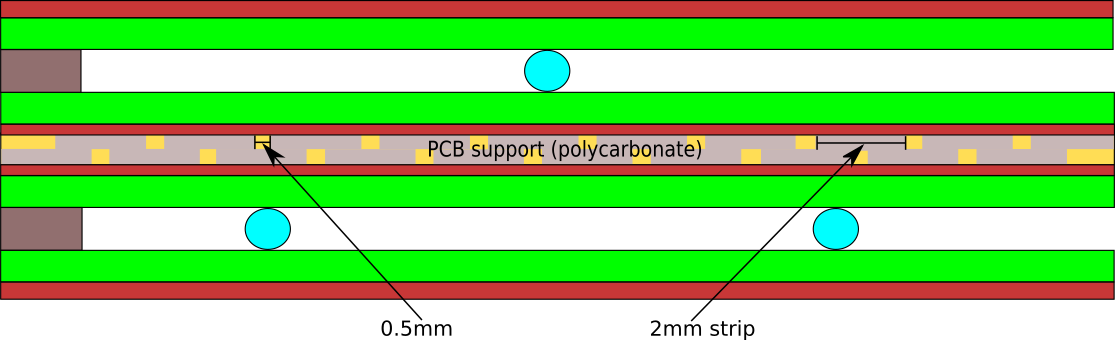
\includegraphics[width=0.9\textwidth]{GLA/DoubleGap.png}
	\captionof{figure}{Schéma de la chambre "double gap" à strips.}
	\label{DoubleGap}
\end{figure}

Deux HARDROC de chaque côté du PCB sont nécessaires pour la lecture des signaux, un des HARDROC lit les strips pairs et l'autre les impairs, ceci afin d'éviter de rendre inefficace une grande partie de la chambre en cas de défaillance de l'une des puces. Pour chaque côté deux DIF sont utilisées, la première sert à récolter et enregistrer le signal, la seconde est reliée à un TDC qui délivre le temps absolu de chaque hit enregistré grâce au signal venant de la sotie OR des HARDROC (cf.fig~\ref{SchemePS}).

\begin{figure}[ht!]
	\centering
	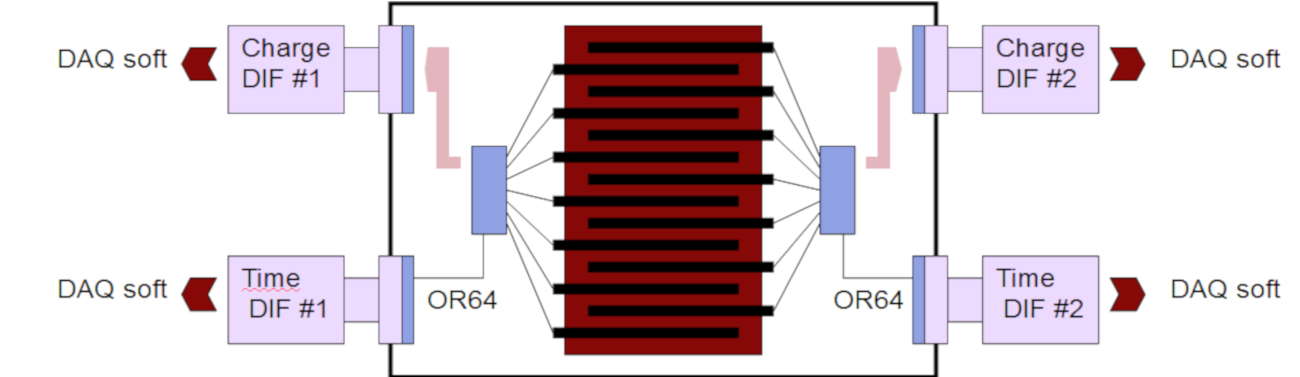
\includegraphics[width=0.93\textwidth]{GLA/SchemePS.png}
	\captionof{figure}{Schéma de la partie électronique de la chambre à strips.}
	\label{SchemePS}
\end{figure}

Le PS fournit des faisceaux d'électrons, de hadrons, de muons... avec une impulsion allant du de \SIrange{1}{15}{\giga\eV}/c. Le faisceau est composé de trains de particules envoyés toutes les \SI{33.6}{\second} en moyenne dans la zone d'expérience. La durée d'un train de particules est d'environ \SI{400}{\milli\second}. le flux de particules est compris entre $1$ et $2.10^{6}$ particules par train de faisceau. Dans notre cas, nous avons utilisé un faisceau de muons (cf.fig~\ref{faisceauPS}).
 
\begin{figure}[ht!]
	\centering
	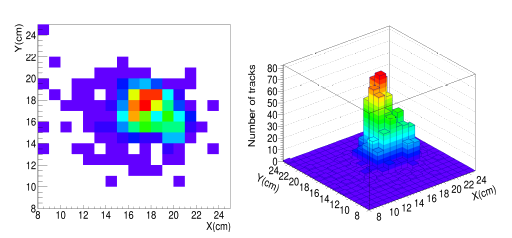
\includegraphics[width=0.83\linewidth]{GLA/FaisceauPS.png}
	\caption{Profil du faisceau dans une chambres à pads reconstruit grâce aux traces. (l'efficacité des chambres n'est pas prise en compte).}
	\label{faisceauPS}
\end{figure}

Un scan en tension pour toutes les chambres a permis de fixer le point de fonctionnement à \SI{7200}{\volt}. Le seuil utilisé est de \SI{0.13}{\pico\coulomb}. Les résultats du scan en tension donnant l'efficacité en fonction de la tension appliquée aux bornes des électrodes pour la chambre à strip sont donnés figure \ref{ScanTensionPS}. Le flux de particules estimé lors de ce scan est de \SI{3.5}{\kilo\hertz\per\square\centi\meter}.

\begin{figure}[!ht]
	\centering
	\scalebox{1.4}{\includetex{GLA/HVPS}}
	\caption{Efficacité en fonction de la haute tension appliquée pour la chambre à strips. Le flux de particules moyen est estimé à \SI{3.5}{\kilo\hertz\per\square\centi\meter}}
	\label{ScanTensionPS}
\end{figure}

Une fois le point de fonctionnement fixé, un scan de l'efficacité en fonction du flux de particules incidentes a été réalisé (cf.fig~ \ref{ScanRatePS}).

\begin{figure}[!ht]
	\centering
	\scalebox{1.4}{\includetex{GLA/RatePS}}
	\caption{Efficacité en fonction du flux de particules. La tension est fixé à \SI{7200}{\volt}.}
	\label{ScanRatePS}
\end{figure}

La multiplicité de la chambre à strips a été utilisée afin d'estimer sa résolution spatiale. Dans le cas ou un seul côté du PCB est touché, un estimateur de la résolution spatiale est :
\begin{equation}
\sigma=\frac{Nd}{\sqrt{12}}
\end{equation}
où $N$ est le nombre de strips touchés dans une zone de $\pm 3$ strips autour du point d’impact de la trace reconstruite, et $d$ le pas des strips.

Quand les deux côtés du PCB sont touchés, seuls les strips se chevauchant sont considérés ce qui permet d'obtenir une estimation plus précise de la résolution spatiale :
\begin{equation}
\sigma=\frac{D}{\sqrt{12}}
\end{equation} 
où $D$ est la distance entre les deux bords les plus éloignés de l'amas constitué des strips se chevauchant.

La multiplicité ainsi que la résolution spatiale calculées en fonction du flux de particules incidentes est donnée figure \ref{ResoSpatialPS}. 

\begin{figure}[!ht]
	\centering
	\scalebox{1.4}{\includetex{GLA/MultiplicityPS}}
	\caption{Multiplicité (axe de gauche) et résolution spatiale (axe de droite) en fonction du flux de particule au point de fonctionnement 7200V.}
	\label{ResoSpatialPS}
\end{figure}

On peut remarquer que la résolution spatiale est améliorée au fur et à mesure de l'augmentation du flux de particules. Elle passe de \SI{1.5}{\milli\meter} à environ \SI{1.1}{\milli\meter} pour $\sim$ \SI{10}{\kilo\hertz\per\square\centi\meter}. L'amélioration de la résolution spatiale en fonction du flux de particules peut s'expliquer par un effet d'écrantage dû à l'accumulation de charges sur les électrodes. Le champ électrique aux bornes s'en trouve diminué ce qui décroit le gain du gaz et donc amène à une réduction de la multiplicité.

\subsection{Tests en faisceaux au SPS} 
Cinq chambres à pads ont ensuite été amenées sur la ligne H2 \cite{H2line} du SPS en Juin 2015. La ligne H2 permet d'obtenir des faisceaux de hadrons, électrons ou muons d'impulsion entre 10 et 360 GeV/c ainsi que des protons primaires de 400 GeV/c. La ligne H2 est situé dans la \textit{North Area} (cf.fig~\ref{complexe}). Tout comme le PS, le faisceau du SPS est composé de trains de particules envoyés toutes les \SIrange{14}{48}{\second} dans la zone d’expérience selon la disponibilité du SPS et de la nécessité de réinjecter du faisceau dans le LHC. La durée d’un train de particules est compris entre \SI{4.8}{\second} et \SI{9.6}{\second}. L'intensité du faisceau peut aller jusqu'à $\sim 2.10^{8}$ particules par train. Dans notre cas un faisceau de muons (et quelques pions) durant environ \SI{7}{\second} a été utilisé (cf.fig~\ref{ProfilFaisceauSPS}).

\begin{figure}[ht!]
	\centering
	\subfloat{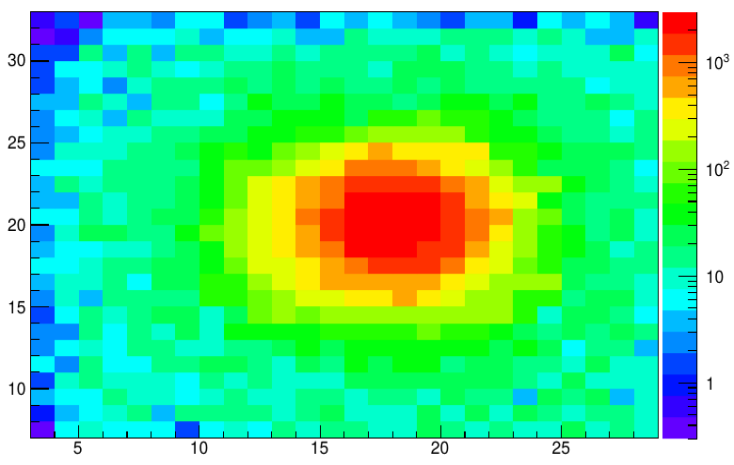
\includegraphics[width=.48\linewidth]{GLA/FaisceauSPS1.png}}
	\hfill
	\subfloat{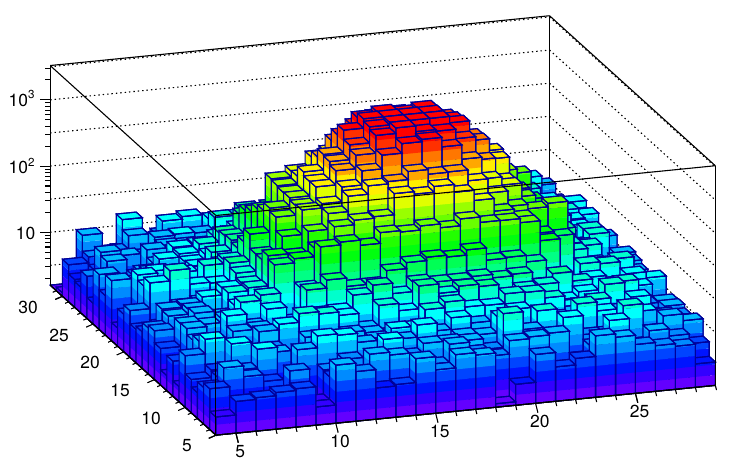
\includegraphics[width=.48\linewidth]{GLA/FaisceauSPS2.png}}
	\caption{Profil du faisceau dans une chambre à pads reconstruit grâce aux traces (l’efficacité des chambres n’est pas prise en compte).}
	\label{ProfilFaisceauSPS}
\end{figure}

De par la structure en train du faisceau, l'efficacité de détection des muons des chambres pourrait être surestimée de façon notable. En effet entre deux trains de faisceau, les charges accumulées dans les chambres lors du train précédent ont le temps d'être évacuées grâce au générateur haute tension. Lors des premiers instants du passage des particules du train suivant, la chambre est donc efficace et enregistre quelques événements avant de voir son efficacité chuter peu à peu. Afin d'empêcher la surestimation de l'efficacité, le processeur Trivent a été modifié afin de détecter la structure en train de faisceau dans les données (cf.fig~\ref{StructureSpill}) et de supprimer les données des deux premières secondes de chaque train de particules.
\vspace*{0.4cm}
\begin{figure}[!ht]
	\centering
	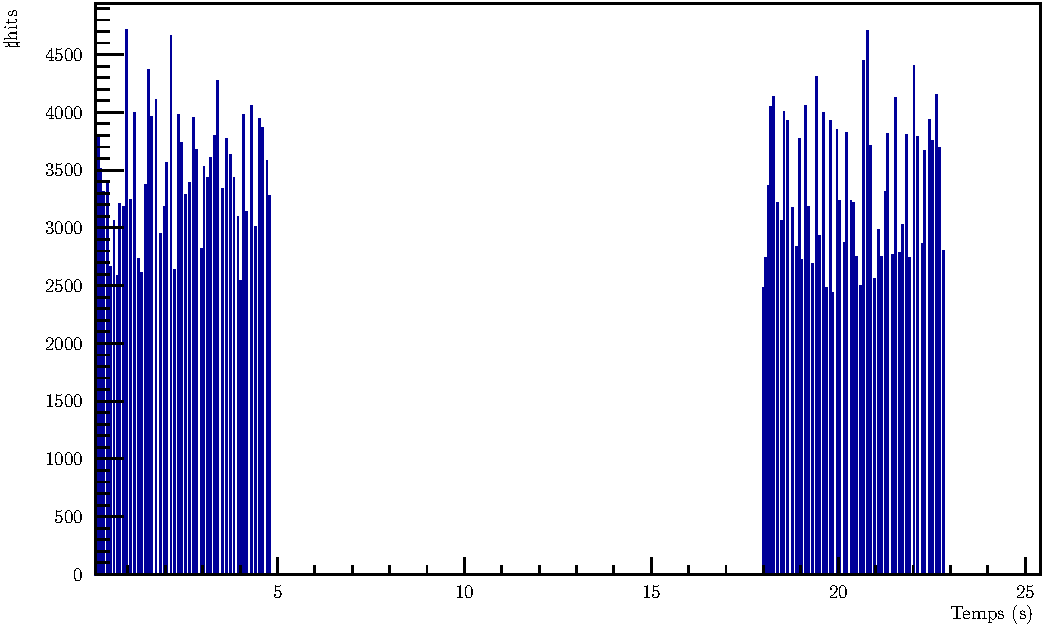
\includegraphics[width=0.93\textwidth]{GLA/SpillStructure.pdf}
	\caption{Structure des trains de faisceau vue par le détecteur. Pour ce fichier, les trains durent \SI{4.8}{\second}.}
	\label{StructureSpill}
\end{figure}

Un scan en tension pour toutes les chambres a d'abord été effectué afin de fixer le point de fonctionnement. Le seuil utilisé est de 0.13pC. Les résultats du scan en tension donnant l’efficacité en fonction de la tension appliquée aux bornes des électrodes pour une des chambres ainsi que la multiplicité sont donnés figure \ref{HVSPS}. Le flux de particules estimé lors de ce scan est de \num{120000} particules par train de faisceau de 7s.

\begin{figure}[!ht]
	\centering
	\scalebox{1.3}{\includetex{GLA/HVSPS}}
	\caption{Efficacité (axe de gauche) et multiplicité (axe de droite) en fonction de la haute tension appliquée.}
	\label{HVSPS}
\end{figure}

On remarque que le plateau est atteint vers \SI{6.7}{\kilo\volt} et que les chambres pour cette tension ont une multiplicité assez faible de $2.2$ hits. 

Une étude de l'efficacité et de la multiplicité en fonction du flux de muons a également été réalisée. Le faisceau présente un profil Gaussien de $\sigma_{x}=\sim 1.4cm$ et $\sigma_{y}=\sim 1.6cm$. Le faisceau du SPS est relativement concentré. Une zone de \num{6}$\times$\SI{6}{\square\centi\meter} contient environ 90\% des muons incidents.

La figure \ref{RateSPS} (\ref{MultiplictySPS}) montre l'évolution de l'efficacité (la multiplicité) en fonction du flux de particules moyen pour les cinq chambres du télescope.

\begin{figure}[!ht]
	\centering
	\scalebox{1.3}{\includetex{GLA/RateSPS}}
	\caption{Efficacité en fonction du flux de particules moyen estimé. Les RPC de basse resistivité sont en bleue et la chambre en verre "standard" est en rouge.}
	\label{RateSPS}
\end{figure}

\begin{figure}[!ht]
	\centering
	\scalebox{1.315}{\includetex{GLA/MultiplicitySPS}}
	\caption{Multiplicité en fonction du flux de particules moyen estimé. Les RPC de basse resistivité sont en bleue et la chambre en verre "standard" est en rouge.}
	\label{MultiplictySPS}
\end{figure}

Comme prévu les cinq chambres ont une efficacité proche de 90\% à bas flux de particules. Cependant l'efficacité de  la chambre en verre "standard" chute brutalement à mesure que le flux augmente et atteint $\sim $40\% à partir de \SI{0.1}{\kilo\hertz\per\square\centi\meter}, en accord avec les données récoltées à DESY. Quant aux chambres en verre de basse résistivité, elles gardent une efficacité supérieure à 70\% dans tous les cas, même à plus de \SI{7}{\kilo\hertz\per\square\centi\meter}. Une des chambres de basse résistivité semble cependant posséder une efficacité beaucoup plus faible que les trois autres. Cette baisse d'efficacité peut s'expliquer d'une part par un nombre de canaux morts dont l'effet n'a pas été pris en compte lors du calcul de l'efficacité. De plus, un verre de plus haute résistivité est sûrement la cause de cet effet. Mis à part cette chambre, les résultats présentés ci-dessus sont en accord avec ceux de DESY.

\section {Tests au Gamma Irradiation Facility (GIF++)}
Jusqu'à présent nous avons effectué des tests en faisceaux de flux assez important ($\sim$ \SI{10}{\kilo\hertz\per\square\centi\meter}). Cependant, ces faisceaux sont bien localisés et ne couvrent pas toute la surface des chambres. Des flux de particules similaires sur toute la surface du détecteur pourraient changer drastiquement les résultats sur l'efficacité et la multiplicité des chambres. En effet, si la surface entière des chambres est soumise à un flux de particules intense, le nombre de charges à évacuer par la haute tension est beaucoup plus importants, ce qui peut conduire à une accumulation de charges et à un effet d'écrantage conduisant à une baisse de l'efficacité. Afin de tester nos chambres dans des conditions plus proches de la situation à laquelle elles seront exposées, nous les avons amenées au Gamme Irradiation Facility (GIF++). De plus, jusqu'à présent, les résultats présentés ont été obtenus en utilisant le mélange de gaz ILC (93\% \chemform{TFE}, 5\% \chemform{CO_2}, 2\% \chemform{SF_6}). Au GIF++, le mélange de gaz de CMS (95.2\% \chemform{TFE}, 4.5\% \chemform{C_4H_{10}}, 0.3\% \chemform{SF_6}) non humidifié sera utilisé.

\subsection{Le GIF++}
Le GIF++ \cite{Jakel:1977147} (cf.fig~\ref{GIF2},cf.fig\ref{GIF}) est une installation de 100$m^2$ installé le long de la ligne de faisceau H4 dans la \textit{North Area} du CERN (cf.fig~\ref{complexe}). Il s'agit d'une installation qui permet à la fois de disposer d'un faisceau de particules (surtout des muons jusqu'à 100GeV/c d'impulsion.) et d'une source de Césium 137 de 14TBq. Cette source permet de baigner la zone d'un fond de $\gamma$ 30 fois supérieur à celui de son prédécesseur, le GIF.

Cette installation a été conçue afin de tester les performances et la stabilité des nouvelles technologies et des nouveaux détecteurs pour le passage du LHC au HL-LHC. L'activité de la source présente au GIF++ permet de tester le vieillissement des détecteurs et d'accumuler une dose équivalente à celle des conditions expérimentales du HL-LHC et ce dans un temps raisonnable ($\sim$ année). 

\marginpar
{
	\centering
	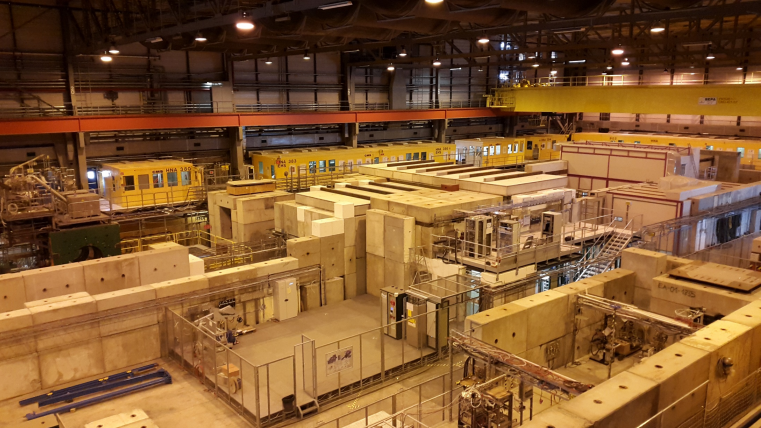
\includegraphics[width=\marginparwidth]{GLA/GIF2.png}
	\captionof{figure}{Vue extérieure du GIF++.}
	\label{GIF2}
}

\begin{figure}[ht!]
	\centering
	\subfloat[Schéma de l'intérieur du Bunker du GIF++]{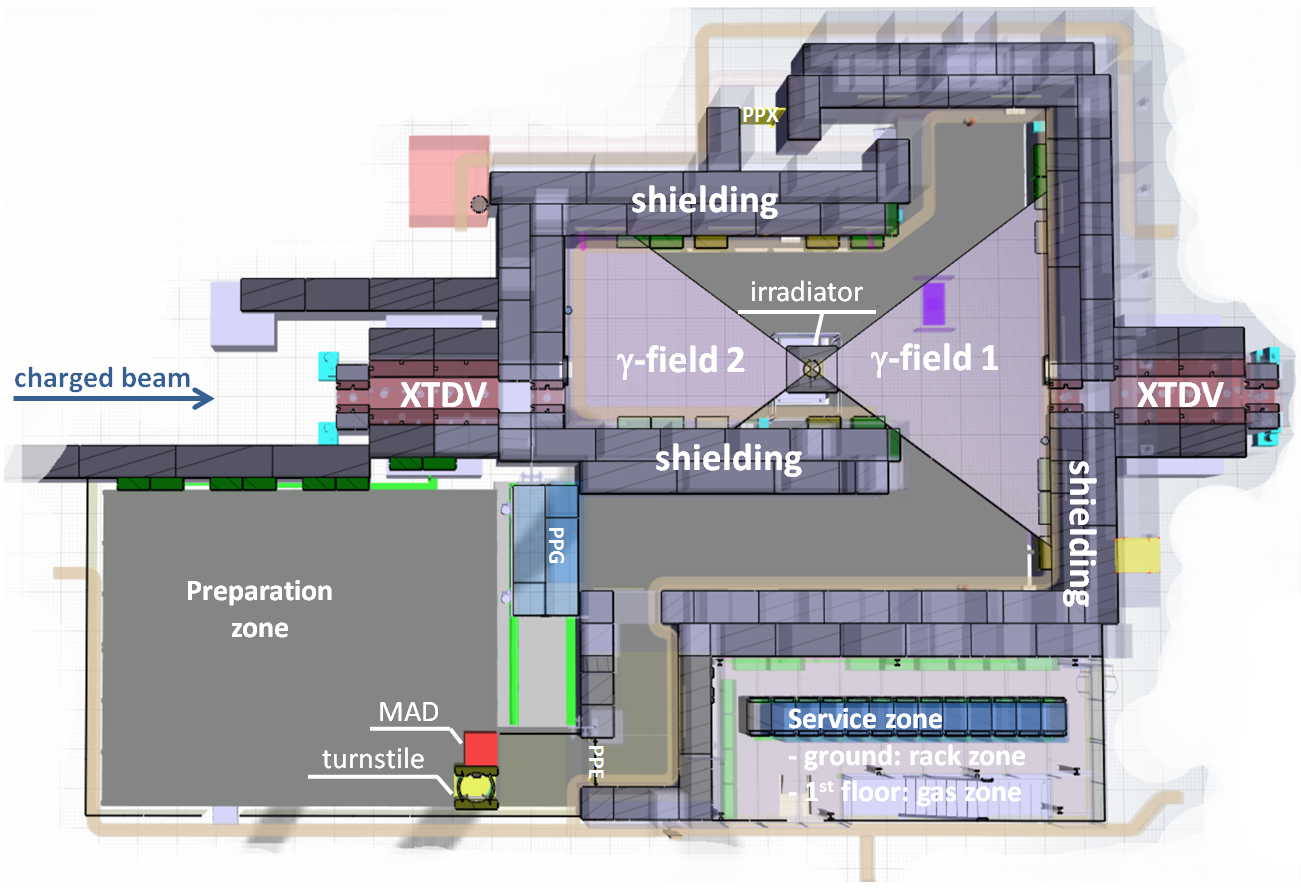
\includegraphics[width=.90\linewidth]{GLA/GIF1.png}\label{GIFa}}
	\hfill
	\subfloat[Vue panoramique de l'intérieur du bunker, (vue face au faisceau \textit{Upstream})]{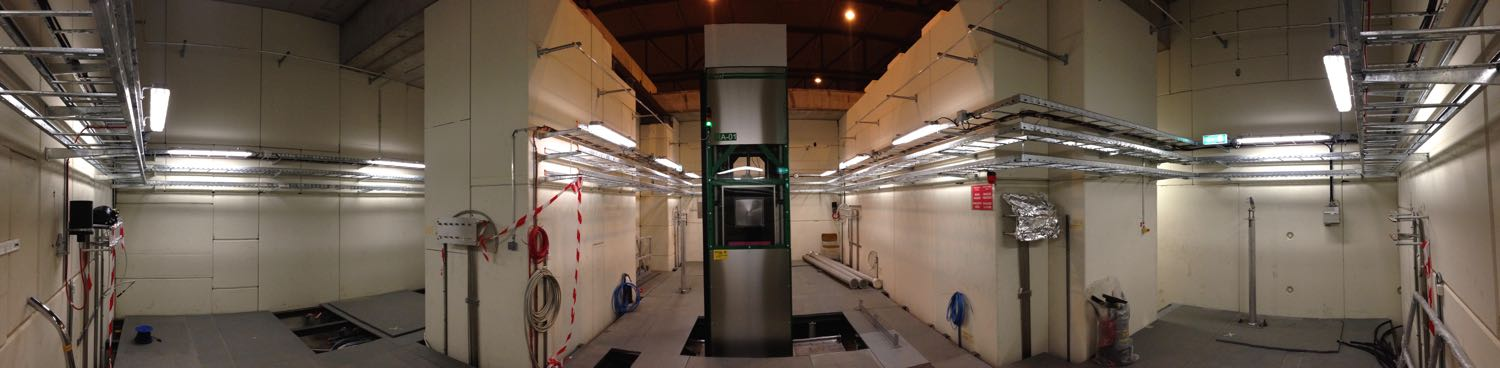
\includegraphics[width=.90\linewidth]{GLA/GIF3.jpg}}
	\caption{Le GIF++.}
	\label{GIF}
\end{figure}


La source de Césium 137 (cf.fig~\ref{Source}) a une demi-vie de 30.08 années et se désintègre selon le diagramme \ref{Diagramme}. Dans 94.6\% il transmute en isomère\footnote{L’isomérie nucléaire est le fait qu'un même noyau atomique puisse exister dans des états énergétiques distincts caractérisés chacun par un spin et une énergie d'excitation particuliers.} $^{137m}$Ba du baryum 137 par désintégration $\beta^{-}$ lequel retombe à son état fondamental par transition isomérique émettant un rayonnement $\gamma$ de 661,7 keV avec une période de 2,552 minutes. Dans les 5,4\% des cas restants, il se désintègre directement en 137Ba avec une énergie de désintégration de 1 174 keV. Cette source est placée dans un irradiateur (cf.fig~\ref{Irradiateur})

\begin{figure}[!ht]
	\centering
	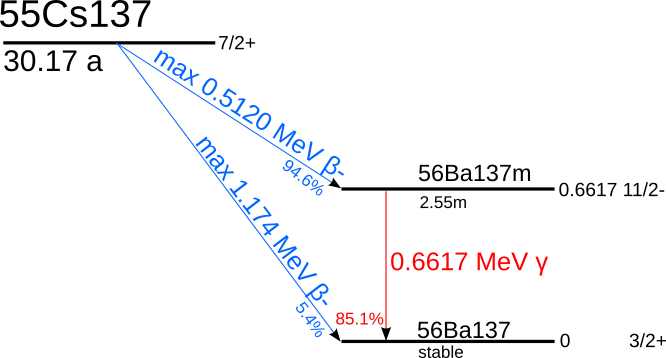
\includegraphics[width=0.69\textwidth]{GLA/Cesium137.png}
	\caption{Diagramme de désintégration du césium 137.}
	\label{Diagramme}
\end{figure}


\marginpar
{
	\centering
	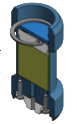
\includegraphics[width=0.5\marginparwidth]{GLA/Source.png}
	\captionof{figure}{Vue en coupe de la source de Césium 137.}
	\label{Source}
}

\marginpar
{
	\centering
	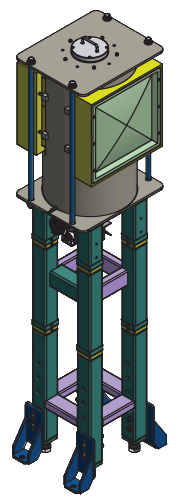
\includegraphics[width=0.5\marginparwidth]{GLA/Irradiateur.png}
	\captionof{figure}{Vue en trois dimensions de l'irradiateur.}
	\label{Irradiateur}
}

L'irradiateur, grâce à des collimateurs, couvre deux zones de $\pm37\degres$ horizontalement et $\pm37\degres$ verticalement (notées $\gamma$-field 1 et $\gamma$-field 2 sur la figure \ref{GIFa}). Ces deux zones sont appellées \textit{Upstream} et \textit{Downstream} selon qu'elles se trouvent proches de l'entrée du faisceau de muons dans le bunker ou non. Elles peuvent être irradiées de manière indépendante grâce à l'emploi de deux systèmes d'atténuateurs, constitués de 3 plans de 3 filtres en plomb chacun (notés A1, B1, C1, A2, B2, C2, A3, B3, C3 sur la figure \ref{SchemeIrradiator}). De chaque côté, les plans peuvent être abaissés et remontés directement depuis la salle de contrôle du GIF++ afin de positionner les bons filtres devant l'irradiateur.

\begin{figure}[!ht]
	\centering
	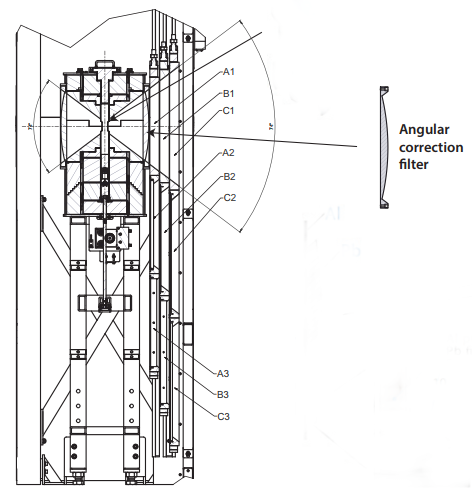
\includegraphics[width=0.6\textwidth]{GLA/SchemeIrradiator.png}
	\caption{Schéma de l'irradiateur et des systèmes d'atténuateurs.}
	\label{SchemeIrradiator}
\end{figure}

La valeur des différents filtres des atténuateurs est donnée dans le tableau \ref{Filter}.
\begin{table}[H]
	\centering
	\begin{tabular}{|O|O|O|O|N}
		\hline 
		Plan  &A&B&C \\ 
		\hline 
		Position 1&1&1&1 \\
		\hline 
		Position 2&10&1.47&2.15 \\ 
		\hline 
		Position 3&100&100&4.64 \\
		\hline
	\end{tabular} 
	\captionof{table}{Tableau des valeurs des filtres des atténuateurs.}
	\label{Filter}
\end{table}

Au total, 24 configurations différentes d'atténuateurs sont possibles, allant d'un facteur d'atténuation de 1 à 46415. Ces facteurs d'atténuation ont été choisis afin d'être à peu prêt équidistants sur une échelle logarithmique sur les trois premiers ordres de grandeur (cf.fig~\ref{ValueAttenuateur} \cite{Pfeiffer:2016hnl}).

\marginpar
{
	\centering
	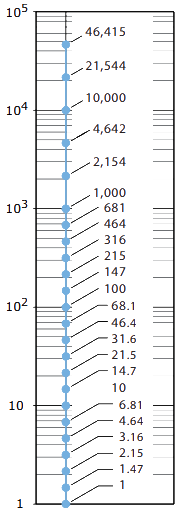
\includegraphics[width=1.0\marginparwidth]{GLA/ValueAttenuateur.png}
	\captionof{figure}{Les 24 valeurs d'atténuations configurables.}
	\label{ValueAttenuateur}
}

Les valeurs nominales des facteurs d'atténuation ont été calculées dans le cas des photons de \SI{662}{\kilo\eV}. Dans le cas des photons de plus basse énergie, les facteurs d'atténuation sont plus élevés. 

Un filtre de correction angulaire en acier est placé de chaque côté de l'irradiateur afin de supprimer la dépendance en $\frac{1}{r^2}$ du courant de photons et de rendre celui-ci uniforme dans le plan xy. Cette correction n'est valable que pour les photons de \SI{662}{\kilo\eV}. Pour les photons de plus basse énergie, créés soit par interaction avec la capsule de la source ou les collimateurs de l'irradiateur, la correction angulaire est beaucoup moins uniforme dans le plan $xy$.

\subsection{Tests en faisceaux (Août 2015)}
À partir de Juillet 2015, le télescope (cf.fig~\ref{GIFppChambers}) à été installé au GIF++ afin de reproduire des conditions de bruits de fond $\gamma$ et ainsi étudier les caractéristiques de ces chambres et le vieillissement de ces chambres sous ces conditions. Les chambres doivent être irradiées pendant plusieurs mois afin d'obtenir une charge intégrée de plus de \SI{1}{\coulomb}, ce qui correspond à la charge accumulée pendant \num{10} ans au HL-LHC.
Plusieurs périodes de tests en faisceaux sont aussi programmées afin de vérifier l'efficacité des chambres et ainsi vérifier la modification de leurs caractéristiques en fonction du temps.

Le télescope est constitué de chambres de verre de basse résistivité et de verre standard afin de servir de témoins. Les chambres sont montées en série dans le circuit de gaz par des tube de polyuréthane. Ces tuyaux permettent une mise en œuvre plus facile et un retrait ou déplacement des chambres plus facile. Tout le système d'alimentation des chambres en basse tension, la SDCC etc est placé dans une boite conçu pour l'occasion (cf.fig~\ref{boite}), placée dans un château de plomb en bas du bâti afin d'éviter les radiations. Cette boite et ses sous composants (basse tension, SDCC) est entièrement contrôlable à distance. Les hautes tensions sont contrôlées par un module CAEN monitorable par telnet.

\marginpar
{
	\centering
	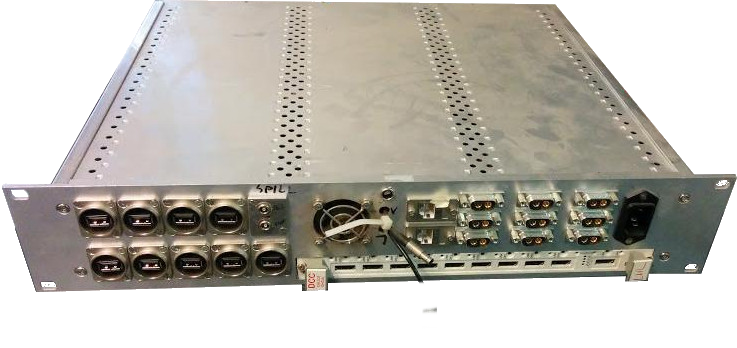
\includegraphics[width=1.0\marginparwidth]{GLA/boite.png}
	\captionof{figure}{Boite contrôlable à distance contenant la SDCC etc.}
	\label{boite}
}

\begin{figure}[!ht]
	\centering
	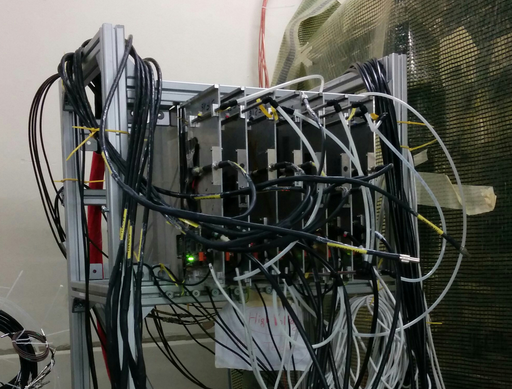
\includegraphics[width=0.55\textwidth]{GLA/GIFppChambers.png}
	\caption{Le télescope dans le bunker du GIF++.}
	\label{GIFppChambers}
\end{figure}

En août 2015, avant le début du vieillissement des chambres un premier test en faisceaux a permis d'avoir des courbes de référence de la tenue des chambres au flux de gamma.

Le télescope a été placé à 2m de la source du côté upstream (cf.fig~\ref{PositionChambre})

\begin{figure}[!ht]
	\centering
	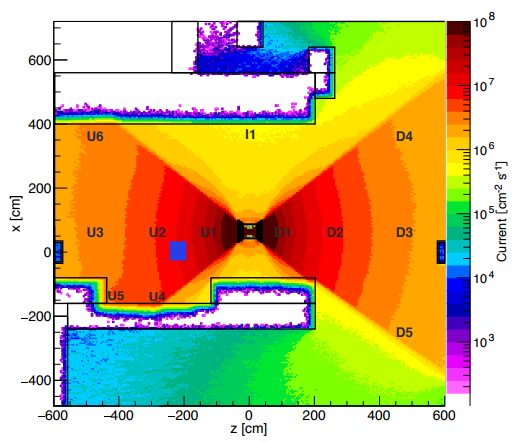
\includegraphics[width=0.55\textwidth]{GLA/PositionChamber.png}
	\caption{courant de photons total ($\gamma$ de toutes énergie de \SIrange{0}{662}{\kilo\eV}) dans le plan $xz$ pour $y=$\SI{0}{\meter}. La position du télescope est indiquée par le carré bleu.}
	\label{PositionChambre}
\end{figure}

Le courant total des photons à l'emplacement du télescope à été estimé de l'ordre de $1.5\times10^{7}\gamma$\si{cm^{-2}.s^{-1}}. Cette estimation peut également varier de quelques \% pour les chambres du telescope placées plus loin de la source. Il est aussi possible d'avoir une variation de quelques pourcents lorsque d'autres détecteurs d'autres expériences se trouvent entre la source et notre télescope.

Lors de ce test en faisceaux, nous avons fait varier les valeurs d'atténuateur de \num{3.16} à \num{46415}. La valeur du point de fonctionnement à été choisie à \SI{7000}{\volt} pour un seuil de \SI{0.13}{\pico\coulomb}. L'évolution de l'efficacité des deux types de chambres en fonction du courant de photons est donnée figure \ref{ATTENUATEURGIF}.

\begin{figure}[!ht]
	\centering
	\scalebox{1.2}{\includetex{GLA/AttenuateurGIF}}
	\caption{Efficacité en fonction du courant de $\gamma$ obtenue pour différentes valeurs d'atténuation de la source. Les effets d'écrantage dus à la présence des autres chambres placées devant ne sont pas inclus.}
	\label{ATTENUATEURGIF}
\end{figure}

Le courant de photons ne donne pas directement le flux de particules qui nous intéresse. En effet, les RPC ne sont sensibles qu'aux particules chargées, il est donc nécessaire d'estimer le taux de conversion des photons en électrons dans la couche de gaz afin de connaitre le vrai flux de particules auquel est soumise la chambre. 


\marginpar
{
	\centering
	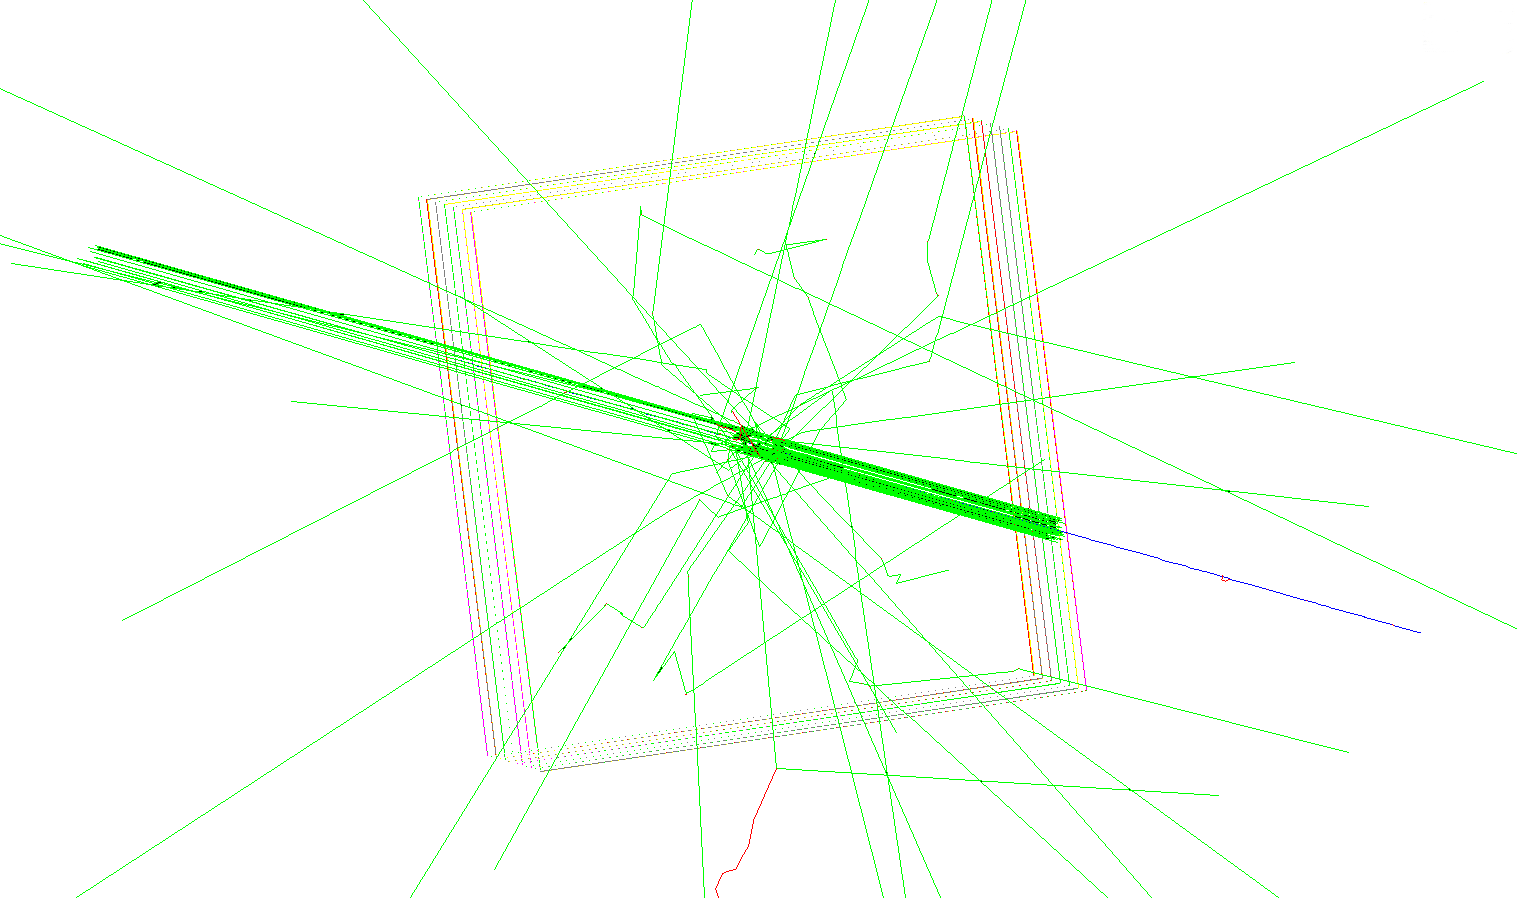
\includegraphics[width=\marginparwidth]{GLA/geant4.png}
	\captionof{figure}{Le passage dans les chambres d'un muon et de photons simulés par GEANT4.}
	\label{GEANT4}
}

Une simulation GEANT4, modélisant le SDHCAL à été modifiée afin de prendre en compte la géométrie des chambres au GIF++ ainsi que leur position relative (cf.fig~\ref{GEANT4}). Un "particle gun" a été utilisé afin de tirer un photon de \SI{661.7}{\kilo\eV} à la fois. Les autres énergies de photons n'ont pas été simulées. La simulation nous permet de connaitre la fraction de photons émis par la source qui produisent un hits dans la couche de gaz des GRPC, ainsi que l'impact des absorptions et diffusions dans les GRPC. La composition exacte des verres de basse résistivité étant inconnue, la simulation se base sur des verres standards. La fraction de photon amenant à la création d'un hit dans les détecteurs, pour plusieurs listes physiques de GEANT 4 est donnée figure \ref{conversion}

\begin{figure}[!ht]
	\centering
	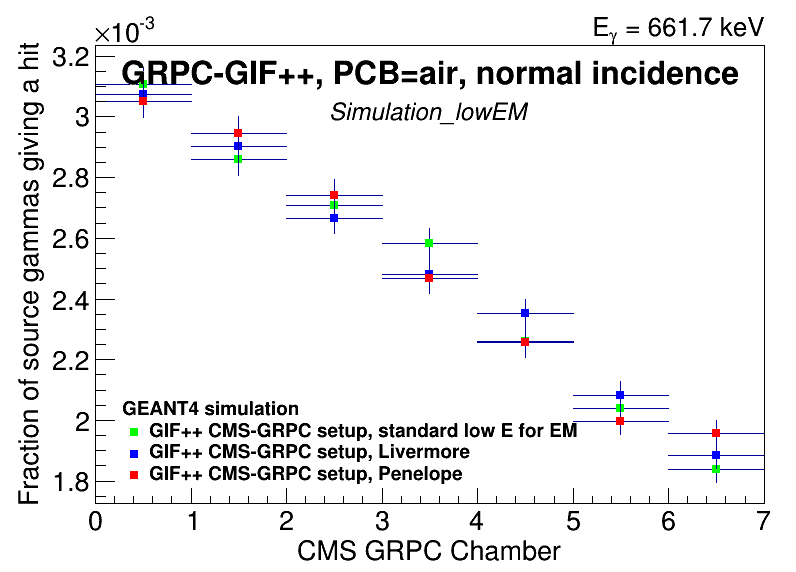
\includegraphics[width=0.50\textwidth]{GLA/taux.png}
	\caption{Taux de conversion : Probabilité qu'un photon de \SI{661.7}{\kilo\eV} produise un hit dans les chambres du télescope au GIF++. Les chambres sont numérotées de \SIrange{0}{6}{}, la chambre \num{0} est la plus proche de la source.}
	\label{conversion}
\end{figure}

Des scans en fonction du seuil appliqué et de la distance à la source ont également été effectués. Les figures \ref{bla1} , \ref{bla2} (\ref{bla3}, \ref{bla4}) représente l'efficacité et la multiplicité en fonction du seuil appliqué pour un facteur d'atténuation de la source de \num{220},\num{22} (\num{150}, \num{46}) dans le cas ou le détecteur est placé à \SI{2}{\meter} (\SI{5.5}{\meter}).

\noindent
\begin{minipage}[th!]{1\textwidth}
	\addtocounter{figure}{1}
	\centering
	\noindent
	\begin{minipage}[th!]{1\textwidth}
		\noindent
		\centering
		\begin{minipage}[th!]{0.49\textwidth}
			\noindent
			\centering
			\renewcommand\thesubfigure{\alph{subfigure}.1}
			\scalebox{0.68}{\includetex{GLA/Eff_200_1970}}
			\vspace*{-0.3cm}
			\captionof{subfigure}{Efficacité en fonction du seuil.}
			\label{att220eff}
			\addtocounter{subfigure}{-1}
		\end{minipage}%
		\hfill
		\begin{minipage}[th!]{0.49\textwidth}
			\noindent
			\centering
			\renewcommand\thesubfigure{\alph{subfigure}.2}
			\scalebox{0.64}{\includetex{GLA/Mul_200_1970}}
			\vspace*{-0.3cm}
			\captionof{subfigure}{Multiplicité en fonction du seuil.}
			\label{att220thre}
			\addtocounter{subfigure}{-1}
		\end{minipage}%
		\vspace*{-0.2cm}
	    \renewcommand\thesubfigure{\alph{subfigure}}
	    \captionof{subfigure}{À \SI{2}{\meter} de la source. Le facteur d'atténuation de la source est de \num{220}.}
	    \label{bla1}
	    \begin{minipage}[th!]{0.49\textwidth}
	    	\noindent
	    	\centering
	    	\renewcommand\thesubfigure{\alph{subfigure}.1}
	    	\scalebox{0.64}{\includetex{GLA/Eff_22_1970}}
	    	\vspace*{-0.3cm}
	    	\captionof{subfigure}{Efficacité en fonction du seuil.}
	    	\label{att22eff}
	    	\addtocounter{subfigure}{-1}
	    \end{minipage}%
	    \hfill
	    \begin{minipage}[th!]{0.49\textwidth}
	    	\noindent
	    	\centering
	    	\renewcommand\thesubfigure{\alph{subfigure}.2}
	    	\scalebox{0.64}{\includetex{GLA/Mul_22_1970}}
	    	\vspace*{-0.3cm}
    		\captionof{subfigure}{Multiplicité en fonction du seuil.}
	    	\label{att22thre}
	    	\addtocounter{subfigure}{-1}
	    \end{minipage}%
		\renewcommand\thesubfigure{\alph{subfigure}}
		\vspace*{-0.2cm}
		\captionof{subfigure}{À \SI{2}{\meter} de la source. Le facteur d'atténuation de la source est de \num{22}.}
		\label{bla2}
	\end{minipage}%
	\hfill
	\begin{minipage}[th!]{1\textwidth}
		\noindent
		\centering
		\begin{minipage}[th!]{0.49\textwidth}
			\noindent
			\centering
			\renewcommand\thesubfigure{\alph{subfigure}.1}
			\scalebox{0.64}{\includetex{GLA/Eff_150_5500}}
			\vspace*{-0.3cm}
			\captionof{subfigure}{Efficacité en fonction du seuil.}
			\label{att150eff}
			\addtocounter{subfigure}{-1}
		\end{minipage}%
		\hfill
		\begin{minipage}[th!]{0.49\textwidth}
			\noindent
			\centering
			\renewcommand\thesubfigure{\alph{subfigure}.2}
			\scalebox{0.64}{\includetex{GLA/Mul_150_5500}}
			\vspace*{-0.3cm}
			\captionof{subfigure}{Multiplicité en fonction du seuil.}
			\label{att150thre}
			\addtocounter{subfigure}{-1}
		\end{minipage}%
	    \renewcommand\thesubfigure{\alph{subfigure}}
	    \vspace*{-0.2cm}
	    \captionof{subfigure}{À \SI{5.5}{\meter} de la source. Le facteur d'atténuation de la source est de \num{150}.}
	    \label{bla3}
		\hfill
	    \begin{minipage}[th!]{0.49\textwidth}
	    	\noindent
	    	\centering
	    	\renewcommand\thesubfigure{\alph{subfigure}.1}
	    	\scalebox{0.64}{\includetex{GLA/Eff_46_5500}}
	    	\vspace*{-0.3cm}
	    	\captionof{subfigure}{Efficacité en fonction du seuil.}
	    	\label{att46eff}
	    	\addtocounter{subfigure}{-1}
	    \end{minipage}%
	    \hfill
	    \begin{minipage}[th!]{0.49\textwidth}
	    	\noindent
	    	\centering
	    	\renewcommand\thesubfigure{\alph{subfigure}.2}
	    	\scalebox{0.64}{\includetex{GLA/Mul_46_5500}}
	    	\vspace*{-0.3cm}
	    	\captionof{subfigure}{Multiplicité en fonction du seuil.}
	    	\label{att46thre}
	    	\addtocounter{subfigure}{-1}
	    \end{minipage}%
		\renewcommand\thesubfigure{\alph{subfigure}}
		\vspace*{-0.2cm}
		\captionof{subfigure}{À \SI{5.5}{\meter} de la source. Le facteur d'atténuation de la source est de \num{46}.}
		\label{bla4}
	\end{minipage}%
    \vspace*{-0.2cm}
    \addtocounter{figure}{-1}
	\captionof{figure}{Efficacité et multiplicité en fonction du seuil appliqué pour la première chambre du télescope. La tension appliquée est de \SI{7000}{\volt}.\label{fig::mainbla}}
\end{minipage}%
%\vspace*{-0.5cm}
%\begin{figure}[ht!]
%	\centering
%	\subfloat[Efficacité en fonction du seuil.]{\scalebox{0.68}{\includetex{GLA/Eff_200_1970}}}
%	\hfill
%	\subfloat[Multiplicité en fonction du seuil.]{\scalebox{0.64}{\includetex{GLA/Mul_200_1970}}\label{att220thre}}
%	\caption{Efficacité et multiplicité en fonction du seuil appliqué pour la première chambre du télescope placée à \SI{2}{\meter} de la source. La tension appliquée est de \SI{7000}{\volt} et le facteur d'atténuation de la source est de \num{220}.}
%	\label{att200}
%\end{figure}
%\vspace*{-1.3cm}
%\begin{figure}[ht!]
%	\centering
%	\subfloat[Efficacité en fonction du seuil.]{\scalebox{0.64}{\includetex{GLA/Eff_22_1970}}\label{att22eff}}
%	\hfill
%	\subfloat[Multiplicité en fonction du seuil.]{\scalebox{0.64}{\includetex{GLA/Mul_22_1970}}\label{att22thre}}
%	\caption{Efficacité et multiplicité en fonction du seuil appliqué pour la première chambre du télescope placée à \SI{2}{\meter} de la source. La tension appliquée est de \SI{7000}{\volt} et le facteur d'atténuation de la source est de \num{22}.}
%	\label{att22}
%\end{figure}
%\vspace*{-0.5cm}
On remarque une baisse significative de l'efficacité pour un même threshold lorsque le flux de particule est trop intense ($\sim$\num{6.8e5}$\gamma$\si{\per\square\centi\meter\per\second} pour \ref{att22eff},\ref{att22thre}) ce qui peut s'expliquer par le phénomène de saturation. On trouve bien une baisse de la multiplicité lorsqu'on augmente le seuil sauf pour la figure \ref{att22thre} dominée par les fluctuations statistiques. L'effet du flux de gammas sur la saturation de la chambre est clairement visible lorsqu'on compare les valeurs de la multiplicité de la chambres placé à \SI{5.5}{\meter} (\ref{att150thre} $\sim$\num{2e4}$\gamma$\si{\per\square\centi\meter\per\second}, \ref{att46thre} $\sim$\num{6.5e4}$\gamma$\si{\per\square\centi\meter\per\second})\footnote{La réduction du flux due aux autres setup placés devant n'est pas prise en compte.} à celles où la chambre est placé à \SI{2}{\meter} (\ref{att220thre} $\sim$\num{6.8e4}$\gamma$\si{\per\square\centi\meter\per\second},\ref{att22thre} $\sim$\num{6.8e5}$\gamma$\si{\per\square\centi\meter\per\second}).

%La figure \ref{att150} (\ref{att46}) représente l'efficacité et la multiplicité en fonction du seuil appliqué pour un facteur d'atténuation de la source de \num{150} (\num{46}) dans le cas ou le détecteur est placé à \SI{5.5}{\meter}.
%\vspace*{-0.8cm}
%\begin{figure}[ht!]
%	\centering
%	\subfloat[Efficacité en fonction du seuil.]{\scalebox{0.64}{\includetex{GLA/Eff_150_5500}}}
%	\hfill
%	\subfloat[Multiplicité en fonction du seuil.]{\scalebox{0.64}{\includetex{GLA/Mul_150_5500}}}
%	\caption{Efficacité et multiplicité en fonction du seuil appliqué pour la première chambre du télescope placée à \SI{5.5}{\meter} de la source. La tension appliquée est de \SI{7000}{\volt} et le facteur d'atténuation de la source est de \num{150}.}
%	\label{att150}
%\end{figure}
%\begin{figure}[ht!]
%	\centering
%	\subfloat[Efficacité en fonction du seuil.]{\scalebox{0.64}{\includetex{GLA/Eff_46_5500}}}
%	\hfill
%	\subfloat[Multiplicité en fonction du seuil.]{\scalebox{0.64}{\includetex{GLA/Mul_46_5500}}}
%	\caption{Efficacité et multiplicité en fonction du seuil appliqué pour la première chambre du télescope placée à %\SI{5.5}{\meter} de la source. La tension appliquée est de \SI{7000}{\volt} et le facteur d'atténuation de la source est de %\num{46}.}
%	\label{att46}
%\end{figure}
\vspace*{-0.2cm}
\section{Création du Electronic LOGbook (ELOG)}
\vspace*{-0.4cm}
À chaque nouvelle prise de données, une entrée dans le Electronic LOGbook (ELOG) \cite{ELOG} du SDHCAL, sorte de cahier de manipulation électronique est créé. Il s'agit d'un démon écrit en C, contenant un serveur web qui lit et écrit les entrées du cahier électronique et les affiche en format HTML. Le ELOG du SDHCAL, contenait quelques informations rudimentaires (numéro du fichier de la prise de données, date de création). Devant le nombre de fichiers à analyser et le nombre de paramètres à garder afin de les analyser, un ELOG plus adapté aux manipulations du GIF++ à été créé. Il a été décidé de garder un ELOG plutôt que de créer une database car l'utilisation est beaucoup plus facile et conviviale (cf.fig~ \ref{ELOG}), et la configuration d'un cahier (logbook) repose sur la création d'un simple fichier texte (elogd.cfg) (voir annexe~\ref{elogd.cfg}). 

\begin{figure}[!ht]
	\centering
	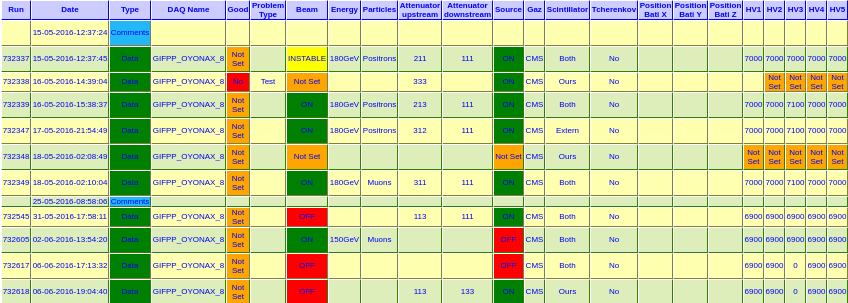
\includegraphics[width=0.75\linewidth]{GLA/ELOG2.png}
	\caption{Cahier de manipulation (logbook) pour les prises de données au GIF++.}
	\label{ELOG}
\end{figure}

Le ELOG du GIF++ contient des menus déroulants et des champs de texte à remplir à chaque nouvelle prise de données. À chaque début de prise de mesure, lors de la création d'une entrée dans le ELOG, la lecture du fichier de configuration XML sur la géométrie du détecteur permet de remplir une bonne partie des informations. Le shifter peut ensuite ajouter les informations manquantes, concernant la source, les atténuateurs, le faisceau etc. La validation d'une entrée ELOG est conditionnée au remplissage des informations les plus utiles selon les circonstances (il est par exemple obligatoire de renseigner les valeurs des atténuateurs si l'état de la source a été sélectionné comme étant "ON"). Cette validation des entrées dans le ELOG permet de s'assurer que la plupart des informations nécessaires à l'analyse des données sont présentes. Toutes ces informations sont ensuite exportables sous format XML ou CSV ce qui rend réalisable la création de programmes sélectionnant les fichiers de données automatiquement en fonction du type de scan que l'on souhaite réaliser (scan en tension, atténuateur etc.)
\vspace*{-0.2cm}
\section{Vieillissement des chambres au GIF++}
\vspace*{-0.4cm}
Afin de valider le choix des verres de basse résistivité comme électrodes, il est nécessaire d'étudier l'impact d'une exposition longue (correspondant à plusieurs années d'utilisation dans CMS) au bruit de fond. La mesure du courant en fonction du temps donne une idée précise du vieillissement des chambres et permet de calculer la charge totale ayant été déposée sur les électrodes. Selon le TDR, les chambres doivent conserver une bonne efficacité même après avoir subi une charge de 1C/cm2. En utilisant la source de photons du GIF++ dont le flux est supérieur de plusieurs ordres de grandeur à celui attendu dans les zones où seront instrumentées les chambres, il est possible d'obtenir la charge intégrée de \SI{1}{\coulomb\per\square\centi\meter} dans un temps raisonnable et ainsi d'accélérer le vieillissement des chambres et ainsi vérifier leur tenue dans le temps.

La figure \ref{CourantLR} (\ref{CourantHR}) montre, les valeurs d'atténuateur, la tension appliquée à la chambre, les courants, la charge intégrées en fonction de la date ainsi que la charge intégrée en fonction du temps effectif pour la chambre de verre standard la plus proche du faisceau (la chambre "float glas" en quatrième position). 

\begin{figure}[!ht]
	\centering
	\subfloat[Valeur de l'atténuateur en fonction du nombre de jours depuis le 1\ier Août 2016.]{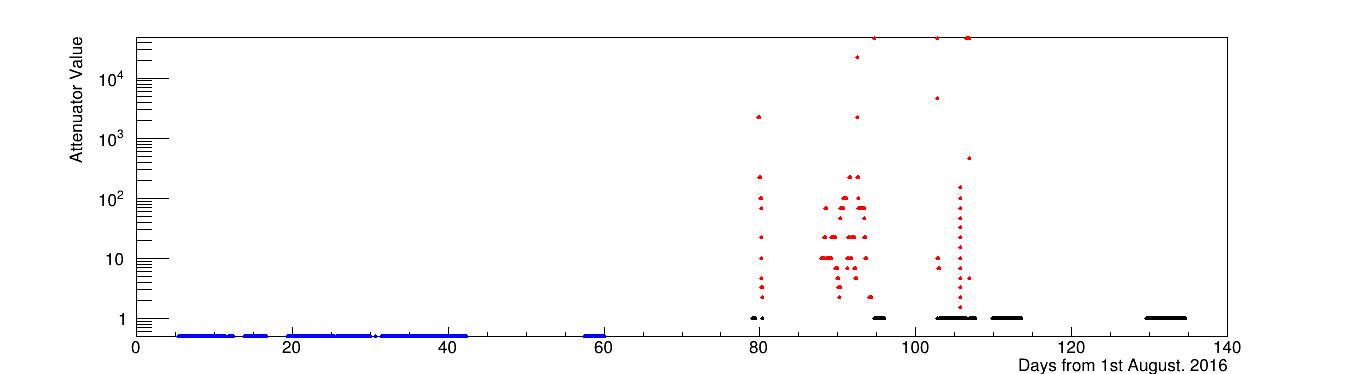
\includegraphics[width=0.82\linewidth]{GLA/current/DIF16_LR_4.png}}
\hfill
\subfloat[Tension appliquée en fonction du nombre de jours depuis le 1\ier Août 2016.]{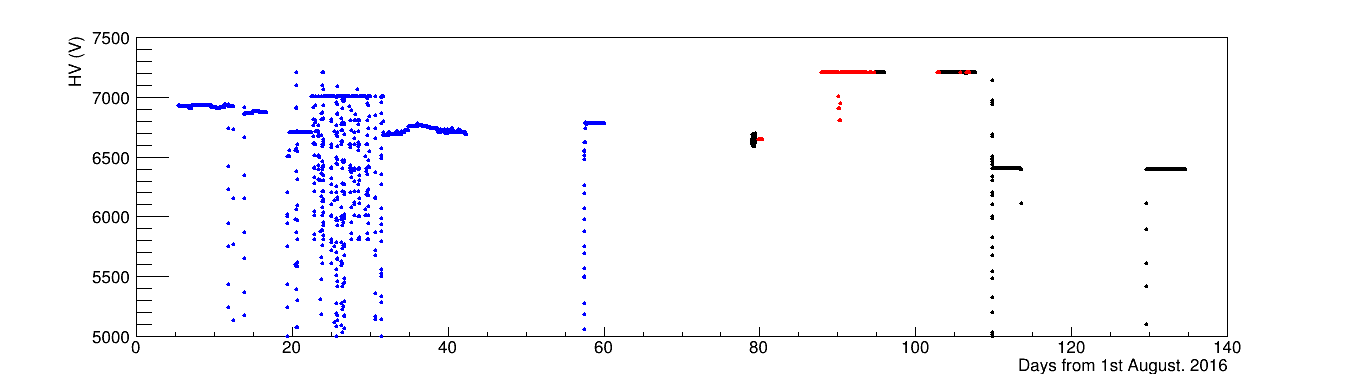
\includegraphics[width=0.82\linewidth]{GLA/current/DIF16_LR_3.png}}
\\
\subfloat[Courant dans la chambre en fonction du nombre de jours depuis le 1\ier Août 2016.]{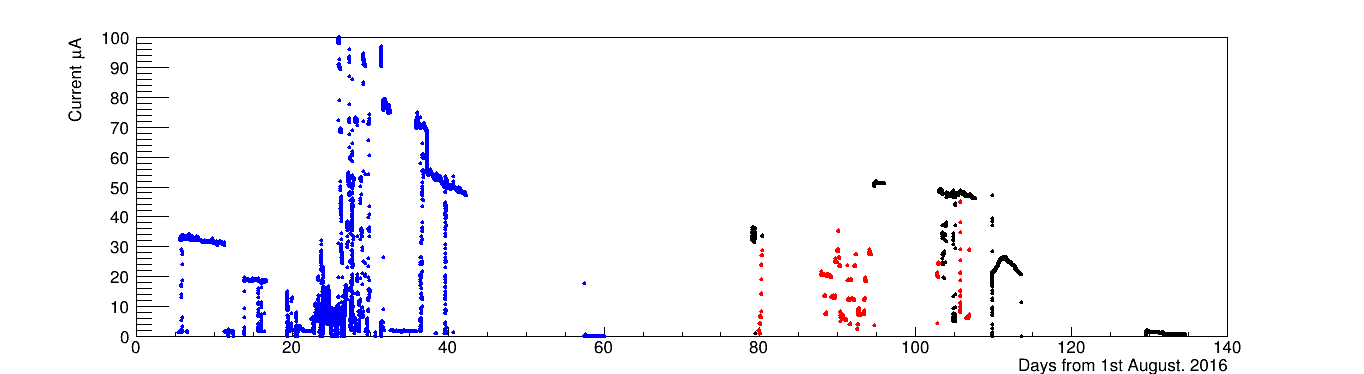
\includegraphics[width=0.82\linewidth]{GLA/current/DIF16_LR_1.png}}
\hfill
\subfloat[Charge intégrée en fonction du nombre de jours depuis le 1\ier Août 2016. ]{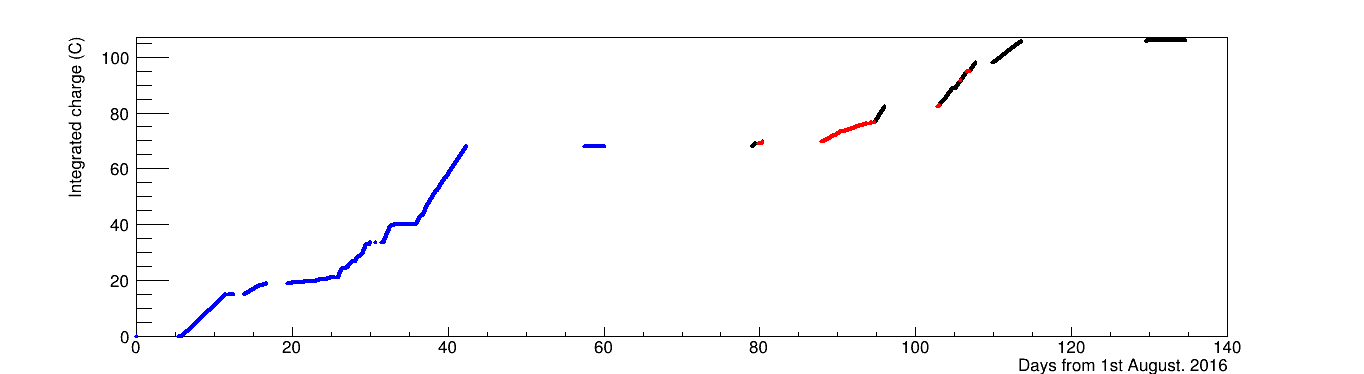
\includegraphics[width=0.82\linewidth]{GLA/current/DIF16_LR_2.png}}
\\
\subfloat[Charge intégrée en fonction du nombres de jours effectifs.]{\includegraphics[width=0.82\linewidth]{GLA/current/DIF16_LR_5.png}}
\caption{Valeur de l'atténuateur, de la tension appliquée, du courant dans les chambres, de la charge intégrée en fonction du nombres de jours depuis le 1\ier Août 2016  et de la charge intégrée en fonction du nombres de jours effectifs pour la chambre de basse résistivité la plus proche de la source.}
	\label{CourantLR}
\end{figure}


\begin{figure}[!ht]
	\centering
	\subfloat[Valeur de l'atténuateur en fonction du nombre de jours depuis le 1\ier Août 2016.]{\includegraphics[width=0.85\linewidth]{GLA/current/DIF32_HR_1.png}}
	\hfill
	\subfloat[Tension appliquée en fonction du nombre de jours depuis le 1\ier Août 2016.]{\includegraphics[width=0.85\linewidth]{GLA/current/DIF32_HR_2.png}}
	\\
	\subfloat[Courant dans la chambre en fonction du nombre de jours depuis le 1\ier Août 2016.]{\includegraphics[width=0.85\linewidth]{GLA/current/DIF32_HR_3.png}}
	\hfill
	\subfloat[Charge intégrée en fonction du nombre de jours depuis le 1\ier Août 2016.]{\includegraphics[width=0.85\linewidth]{GLA/current/DIF32_HR_4.png}}
	\\
	\subfloat[Charge intégrée en fonction du nombre de jours depuis le 1\ier Août 2016.]{\includegraphics[width=0.85\linewidth]{GLA/current/DIF32_HR_5.png}}
	\caption{Valeur de l'atténuateur, de la tension appliquée, du courant dans les chambres, de la charge intégrée en fonction du nombres de jours depuis le 1\ier Août 2016  et de la charge intégrée en fonction du nombres de jours effectifs pour la chambre de "float glass" situé en deuxième position en partant de la source.}
	\label{CourantHR}
\end{figure}

La chute du courant en fonction du temps de manière rapide montre un vieillissement prématuré des chambres. Le test en faisceau de mai 2016 a permis de comprendre les causes de ce vieillissement rapide.

\subsection{Tests en faisceaux (Mai-Juin 2016)}
La structure des hits rejetés par Trivent pour les cinq chambres pour un facteur d'attenuation de la source de \num{22} est donnée figure \ref{struc}
\begin{figure}[ht!]
	\centering
	\subfloat[Chambre \num{1}.]{\includegraphics[width=.48\linewidth]{GLA/chamber5.png}}
	\hfill
	\subfloat[Chambre \num{2} (float glass).]{\includegraphics[width=.48\linewidth]{GLA/chamber4.png}}
	\\
	\vspace{0.4cm}
	\subfloat[Chambre \num{3}.]{\includegraphics[width=.48\linewidth]{GLA/chamber3.png}}
	\hfill
	\subfloat[Chambre \num{4}.]{\includegraphics[width=.48\linewidth]{GLA/chamber2.png}}
	\\
	\vspace{0.4cm}
	\subfloat[Chambre \num{5} (plus éloignée de la source).]{\includegraphics[width=.50\linewidth]{GLA/chamber1.png}}
	\caption{Hits rejetés par Trivent (\si{\hertz}) pour les cinq chambres du télescope au GIF++. La chambre \num{5} est la plus éloignée du faisceau. La chambre \num{4} est une chambre construites en verre standard.}
	\label{struc}
\end{figure}

Les chambres \num{3}, \num{4} et \num{5} présentent de nombreuses zones sans aucun hits. Ces zones sont proches des bords qui continuent de posséder des hits à cause des courants de fuites. La différences de comportements entre les chambres de basses résistivité et la chambre "float glass" est clairement visible. Le nombre de hits rejetés par Trivent\footnote{C'est à dire une bonne partie des hits de bruits} est beaucoup moins importants pour la chambre "float glass". Ceci tend à montrer que l'effet de saturation est beaucoup plus important pour cette chambre que pour les chambres de basse résistivité.

\subsubsection{Étude des courants des chambres}
Des mesures du courant des chambres en fonction du facteur d'atténuation ont été effectuées afin d'avoir une idée plus précise du comportement des chambres en fonction du flux de particules (cf.fig~\ref{courant})

\begin{figure}[ht!]
	\centering
	\subfloat[Chambre 1 (verre de basse résistivité).]{\includegraphics[width=.45\linewidth]{GLA/current_cha5.png}}
	\hfill
	\subfloat[Chambre 2 ("float glass")]{\includegraphics[width=.45\linewidth]{GLA/current_cha4.png}}
	\caption{Intensité parcourant les chambres en fonction de la haute tension appliquée pour différentes valeurs du facteur d'atténuation de la source.}
	\label{courant}
\end{figure}


Les courants des chambres de basse résistivité ont tous le même comportement et présentent un profil non linéaire contrairement à la chambre "float glass".

La figure \ref{currentsamHV} montre le courant parcourant les chambres de basse résistivité et "float glass" en fonction de l'inverse du facteur d'atténuation de la source pour une même valeur de haute tension \SI{6900}{\volt}.

\begin{figure}[ht!]
	\centering
	\includegraphics[width=.75\linewidth]{GLA/current_same_HV.png}
	\caption{Courant (\si{\micro\ampere}) parcourant la chambre de basse résistivité la plus proche de la source (bleue) et "float glass" (orange) en fonction de l'inverse du facteur d'atténuation. La tension appliquée est fixe et de 6900V.}
	\label{currentsamHV}
\end{figure}

On remarque que le courant dans les chambres de basse résistivité est toujours plus élevé que pour la "float glass". Une partie est due à l'effet d'écrantage produit par la présence de la chambre de basse résistivité placée devant la "float glass". On remarque également que la saturation du courant arrive beaucoup plus tôt pour la "float glass" (facteur d'atténuation 68.1) que pour la chambre de basse résistivité qui semble ne pas saturer même pour un facteur d'atténuation de \num{4.64}.

\subsubsection{Estimation de la résistivité des életrodes}

Le GIF++ permet également de faire circuler dans les chambres de l'argon afin de les purger et de les nettoyer. L'argon permet également de mesurer la résistivité des électrodes des chambres. Grâce à ce gaz, les chambres fonctionnent rapidement en mode streamer, la résistance de la couche de gaz devient négligeable  par rapport à la résistance des électrodes. 

L'étude des courants des chambres en fonction de la tension a montré que les verres de basse résistivité possèdent une hystérésis du courant contrairement aux chambres "float glass" (cf.fig~\ref{hysteresis}). L'allure de la courbe montre également que les verres de basse résistivité on un comportement qui n'est pas ohmique contrairement au verre "float glass".


\begin{figure}[ht!]
	\centering
	\subfloat[Chambre 1 (verre de basse résistivité).]{\scalebox{1.2}{\includetex{GLA/Argon_current_chamber_1}}}
	\\
	\subfloat[Chambre 2 ("float glass")]{\scalebox{1.2}{\includetex{GLA/Argon_current_chamber_2}}}
	\caption{Plusieurs scans en montée et en descente  des courants circulant dans la chambre en fonction de la haute tension. La chambre de basse résistivité présente une hystérésis.}
	\label{hysteresis}
\end{figure}


La figure \ref{ScanArgon} montre la variation du courant en fonction de la tension appliquée sur les chambres sous Argon. Un ajustement linéaire est effectué afin d'en déduire la conductance des électrodes.

\begin{figure}[!ht]
	\centering
	\scalebox{1.50}{\includetex{GLA/Argon_current}}
	\caption{Courant circulant dans les chambres en fonction de la tension appliquée. Le gaz utilisé est l'Argon. Les résultats de l'ajustement de la partie linéaire sont également donnés.}
	\label{ScanArgon}
\end{figure}

À partir de la résistance des électrodes il est possible d'en déduire leur résistivité par la formule :
\begin{equation}
\rho=\frac{RS}{e}
\end{equation}
avec $R$ la résistance de l'électrode, $S$ sa surface et $e$ l'épaisseur totale des électrodes.

Le tableau \ref{resistivite} donne la résistivité des chambres calculée grâce à l'ajustement linéaire des courbes de la figure \ref{ScanArgon}.

\vspace{0.7cm}
\begin{table}[H]
	\centering
	\begin{tabular}{|O|O|N}
		\hline 
		Chambre 1 (basse résistivité)  &\SI{2.4e11}{\ohm.\centi\meter} \\ 
		\hline 
		Chambre 2 ("float glass") & \SI{3.60e12}{\ohm.\centi\meter} \\ 
		\hline 
		Chambre 4 (basse résistivité)& \SI{2.49e11}{\ohm.\centi\meter}\\ 
		\hline 
		Chambre 5 (basse résistivité) &\SI{3.94e11}{\ohm.\centi\meter} \\
		\hline
	\end{tabular} 
	\captionof{table}{Résistivité des différentes chambres.}
	\label{resistivite}
\end{table}

La résistivité des chambres de basse résistivité est beaucoup plus élevée qu'attendue ($\sim$\SI{e10}{\ohm.\centi\meter}). Toutes ces constatations (fig.\ref{CourantLR}, fig.\ref{struc}, tab.\ref{resistivite}) nous ont amené à ouvrir une chambre afin d'essayer de comprendre ces résultats.
\vspace{0.4cm}
\newpage
L'ouverture d'une des chambres a montré que les spacers permettant le maintien des électrodes à une distance uniforme le long de la chambre ont disparu et qu'un dépôt s'est créé sur les électrodes de la chambre (cf.fig~\ref{depot}). Ces deux constatations peuvent expliquer les structure étonnantes de la distribution des hits rejetés par Trivent. En effet, sans spacer les parties centrales des électrodes se trouvent attirées l'une vers l'autre, ce qui a tendance à augmenter le champ électrique dans cette zone et donc le nombre de hits. La présence de dépôts permet également d'expliquer le fait que certaines zones de la chambre soient aveugles ainsi que la résistivité élevée de ces chambres.

\begin{figure}[!ht]
	\centering
	\includegraphics[width=0.99\textwidth]{GLA/depot.jpg}
	\caption{Vue intérieure d'une chambre du télescope du GIF++. Les spacers ont disparu et un dépôt s'est formé sur les électrodes.}
	\label{depot}
\end{figure}

\subsection{Causes connues du vieillissement des RPC }
Plusieurs causes du vieillissement prématuré des chambres RPC peuvent être trouvées dans la littérature :

\subsubsection{La contamination par l'eau}
Après quelques semaines de prises de données, les GRPC du sous-système $K_{L}/\mu$ de l'expérience BELLE ont perdu une grande partie de leur efficacité ainsi qu'une augmentation du bruit de fond. Les physiciens de cette expérience se sont aperçus en analysant la sortie de certaines chambres que le gaz avait une concentration d'eau allant jusqu'à \num{2000}ppm. La cause de cette concentration d'eau s'avéra être la migration de la vapeur d'eau de l'air ambiant  vers les tubes de polyoléfine de plusieurs mètres de long amenant le gaz dans les chambres. La solution trouvée fût le remplacement de ces tuyaux par des tuyaux de cuivre \cite{Abashian:2000vb}. D'autres études démontrent les effets de la vapeur d'eau sur le vieillissement des électrodes de verre notamment en présence de fréon (l'un des noms du \chemform{TFE} est Freon 134a) \cite{Sakai:772080}, \cite{Kubo:2002jq}.

\newpage
Bien qu'ayant utilisé des tuyaux de polyamide, qui présente un coefficient d'absorption faible en présence d'humidité et une bonne résistance aux radiations, nous avons décidé de remplacer ces tuyaux par des tuyaux en cuivre. Le choix des tuyaux en polyamide s'était imposé pour leur facilité d'utilisation (découpe, remplacement etc.). 

\subsubsection{La polymérisation de l'isobutane}
 L'isobutane \chemform{iC_4H_{10}} appartient à la classe des alcanes. Il est connu pour produire des réactions de polymérisation, ce qui entraine un dépôt dans les chambres \cite{na60}. L'isobutane est également très inflammable ce qui complique son utilisation en laboratoire. C'est l'une des raisons du choix de son remplacement par du \chemform{CO_2} dans le prototype SDHCAL et également de son utilisation hors du GIF++, de plus le \chemform{CO_2} ne crée pas de dépôt supplémentaire.

\subsubsection{L'attaque du verre par l'acide fluorhydrique \texorpdfstring{\chemform{HF}}{HF}}
L'acide fluorhydrique \chemform{HF} provient de la décomposition du \chemform{TFE} lors de l'ionisation en avalanche. Des études ont montré qu'en mode streamer la production de \chemform{HF} est comprise entre \num{1.19e19}\chemform{F^{-}}\si{\per\coulomb} \cite{Lu:2009zzd} et $\sim$\num{3e19}\chemform{F^{-}}\si{\per\coulomb} \cite{Abbrescia:2006hk} (\num{1.3e19}\chemform{F^{-}}\si{\per\coulomb} pour \cite{Aielli:2006ih}). Ce composant chimique, très corrosif peut même dissoudre le verre selon la réaction :
\begin{chemeqn}
SiO_2+6 HF\longrightarrow H_2SiF_6+H_2O
\end{chemeqn}
L'acide hexafluorosilicique ou fluorosilicique (\chemform{H_2SiF_6}) se retrouve ainsi présent sous forme de dépôt aqueux sur les surfaces internes des électrodes amenant à une diminution de la résistivité de surface de ces parois. Cet acide également corrosif peut attaquer également le verre et détériorer l'état de surface des verres. Les défauts de surface conduisent à une déformation du champ électrique à cause notamment de l'effet de pointe et augmentent ainsi le taux de bruit dans les chambres. Ce qui accélère à son tour la production de \chemform{HF}, créant un processus en chaine.

Ces attaques des électrodes par les composés fluorés peuvent également faire varier la résistivité volumique du matériau et donc modifier sa fréquence maximale de détection.

Il a été montré que la création de l'acide \chemform{HF} est proportionnelle à la charge parcourant les électrodes. Le mode de fonctionnement avalanche permet donc de limiter la création de cet acide. De plus, la circulation du gaz dans les chambres permet d'évacuer une partie des composés fluorés. Dans CMS, la moitié du \chemform{HF} produit est évacué en faisant circuler le gaz dans les chambres avec un débit permettant de remplacer le volume de gaz des chambres une fois par heure \cite{Abbrescia:2006hk}. Les dépôts fluorés absorbés à la surface du verre peuvent également être libérés en utilisant de l'argon pur \cite{Band:2008zza}.

Afin de limiter les dépôts dans nos chambres, nous avons donc essayé d'augmenter le débit de gaz. Cependant, cette augmentation s'est révélée impossible car le débit total du gaz CMS permis au GIF++ doit être partagé avec toutes les autres expériences utilisant ce gaz.
Nous avons également remarqué que certaines de nos chambres comportaient des fuites, ce qui amenait de l'humidité lors des arrêts de gaz par exemple. De plus, les chambres étant montées en série, cette configuration pouvait augmenter la résistance du système. Certaines chambres pouvaient ainsi gonfler et augmenter les fuites diminuant le débit de gaz introduit dans les chambres suivantes. Afin de pallier ce problème, nous avons décidé de passer les chambres en parallèle et de placer à chaque entrée des chambres un débitmètre à vanne de régulation afin d'ajuster le débit de chaque chambre afin de vérifier que chacune d'elles possédait une circulation de gaz.

Au vu de l'état des chambres, il a été décidé de construire de nouvelles chambres de basse résistivité de taille \SI{32}{\centi\meter}$\times$\SI{30}{\centi\meter}. Malheureusement seuls \num{4} verres nous sont arrivés en bon états, ce qui permit de ne créer que deux nouvelles chambres. Ce nombre étant insuffisant pour une étude du vieillissement, nous avons décidé de les utiliser afin d'instrumenter une chambre double gap avec l'électronique présentée figures \ref{DoubleGap} et \ref{SchemePS}. Un même type de PCB à été utilisé afin de créer une chambre avec des électrodes en Bakélite de \SI{2}{\milli\meter} d'épaisseur et un gap de \SI{2}{\milli\meter}. Les résultats de ces tests sont présentés section \ref{smallchamber}.

\newpage
\section{Les chambres de basse résistivité de taille RE1/1}

\marginpar
{
	\centering
	\includegraphics[width=1.0\marginparwidth]{GLA/gaps.png}
	\captionof{figure}{Schèma de la segmentation en gap des prototypes \cite{gapss}.}
	\label{gap}
}

\begin{wrapfigure}[21]{R}{0.40\textwidth}
	\vspace*{-1cm}
	\centering
	\includegraphics[width=0.37\textwidth]{GLA/strips.jpg}
	\caption{Les \num{4} partitions de \num{32} strips selon $\eta$.}
	\label{strips}
\end{wrapfigure}

En parallèle à la caractérisation des chambres de basse résistivité, l'étude de la faisabilité de chambres de grande dimension (reprenant de nombreuses caractéristiques des chambres RE1/1 \cite{gapss}) a été effectué. En effet, la limitation par la méthode de production de la taille des verres de basse résistivité nécessite de trouver une manière efficace et robuste d'assembler ces verres.  Deux prototypes basés sur deux méthodes d'assemblage différentes des verres de \SI{32}{\centi\meter}$\times$\SI{30}{\centi\meter} ont été réalisés. Les chambres sont constituées de trois gap (cf.fig~\ref{gap}). Un PCB, placé entre les gaps du bas et celui du haut, possédant \num{4} rangées de \num{32} strips de $\sim$\SI{1}{\centi\meter} est utilisé afin de récolter le signal (cf.fig~\ref{strips}). Pour les deux prototypes, l'assemblage des verres est prévu de manière à éviter les zones mortes. Les deux prototypes ont été réalisés avec des verres "float glass" afin de limiter l'utilisation de verre de basse résistivité. La solution retenue sera ensuite produite avec des verres de basse résistivité.

\subsection{Les différentes méthodes d'assemblages} 
\subsubsection{Méthode par collage}
La première méthode consiste à coller les verres entre eux grâce à de la colle RHODORSIL\textsuperscript{\textregistered}
 CAF-4 afin de former les électrodes. La zone de collage est inférieure à \SI{100}{\micro\meter}. La peinture résistive est ensuite appliquée sur l'électrode ainsi formée (cf.fig~\ref{a}). Les trois gaps sont hermétiques (cf.fig~\ref{b}) et placés dans une cassette en aluminium (cf.fig~\ref{c}).
 
 \begin{figure}[ht!]
 	\centering
 	\begin{minipage}[t]{.45\textwidth}
 	\centering
 	\vspace*{1.cm}
 	\subfloat[Gap (i) hermétique formé par collage des verres. On voit clairement les zones de collage.]{\includegraphics[width=1\textwidth]{GLA/Glass-glued.png}\label{a}}
 	\end{minipage}
    \hfill
    \begin{minipage}[t]{.45\textwidth}
    \centering
    \subfloat[Gap (ii) et Gap(iii) hermétique formé par collage des verres dans la cassette evec les strips et le gap(i) au dessous.]{\includegraphics[width=1\textwidth]{GLA/Glass-glued2.png}\label{b}}
    \\
    \vspace*{1cm}
    \subfloat[La cassette fermée.]{\includegraphics[width=1\textwidth]{GLA/cassette_colle.jpg}\label{c}}
    \end{minipage}
 	\caption{Photos des gaps et de la cassette. Les entrées et sorties de gaz sont les tuyaux bleus et rouge. La haute tension est amenée par les câbles blancs.}
 	\label{colle}
 \end{figure}
 
 \subsubsection{Méthode par fixation mécanique}
 La deuxième méthode permet de se passer de colle, celle-ci pouvant se détériorer sous les radiations. Les carreaux de verre sont tenus par des plots placés sur les pourtours de la cassette en aluminium (cf.fig~\ref{aa}, \ref{posverre}). Les verres sont reliés électriquement par des adhésifs en cuivre et forment ainsi les électrodes (cf.fig~\ref{cc}). Le gap entre les électrodes est assuré par des fils de pêche perlés (cf.fig~\ref{bb}). Une plaque de poly(méthacrylate de méthyle) (PMMA) de la même taille que l'intérieur de la chambre est équipée de plusieurs ressorts qui une fois le capot posé, assurent le maintient et la planéité des verres sur le PCB.  Avec cette méthode, l'herméticité est assurée par la cassette (cf.fig~\ref{dd}), les électrodes d'un gap ne sont donc pas reliées entre-elles. Le gaz circule donc dans toute la chambre et pas seulement entre les électrodes comme pour la méthode précédente.
 
 \begin{figure}[ht!]
 	\centering
 	\subfloat[Les différents verres formant un gap.]{\includegraphics[width=0.45\textwidth]{GLA/meca1.jpg}\label{aa}}
 	\hfill
 	\subfloat[Les plots assurant le maintien des verres ainsi que les fils de pêche assurant l'espace entre les électrodes d'un gap.]{\includegraphics[width=0.45\textwidth]{GLA/meca2.png}\label{bb}}
 	\\
 	\subfloat[Pose du PCB au dessus du gap du bas. On peut remarquer, par transparence, les adhésifs de cuivre (encadrés en rouge sur la figure) reliant électriquement les verres d'un gap.]{\includegraphics[width=0.45\textwidth]{GLA/meca3.png}\label{cc}}
 	\hfill
 	\subfloat[La cassette fermée hermétiquement.]{\includegraphics[width=0.45\textwidth]{GLA/meca4.png}\label{dd}}
 	\\
 	\subfloat[Schéma de la cassette.]{\includegraphics[width=0.45\textwidth]{GLA/posverre.pdf}\label{posverre}}
 	\caption{Photos et schéma du prototype de cassette construite selon la méthode par fixation mécanique.}
 	\label{meca}
 \end{figure}
 
 \subsection{Comparaison des deux méthodes de constructions}
 
 Afin de pouvoir comparer les deux méthodes de construction, un banc cosmique à été mis en place afin de vérifier l'efficacité des deux prototypes.
 
 \subsubsection{Le banc de test cosmique}
 \label{banc}
 La Terre est constamment bombardée par des particules composant le rayonnement cosmique. Ce rayonnement est un flux de noyaux atomiques et de particules de haute énergie circulant dans le vide interstellaire. La plupart d'entre elles interagissent avec l'atmosphère terrestre et produisent des gerbes atmosphériques de particules secondaires (cf.fig~\ref{gerbe2}).
 
 Au niveau du sol, le flux de particules est principalement composé de muons (cf.fig~\ref{flux}) ($\sim$\SI{100}{\per\square\meter\per\second\per\steradian}), ceux-ci interagissant très faiblement avec la matière.
 
\vspace{0.5cm}
\noindent
\begin{minipage}[t]{.44\textwidth}
\noindent
\centering
\includegraphics[width=1\textwidth]{GLA/Gerbe.png}
\captionof{figure}{Schéma d'une cascade atmosphérique produite par un proton.}
\label{gerbe2}
\end{minipage}%
\hfill
\begin{minipage}[t]{.54\textwidth}
\noindent
\centering
\includegraphics[width=0.70\textwidth]{GLA/muon_rate.eps}
\captionof{figure}{Composition du flux cosmique dans l'atmosphère terrestre pour des particules ayant une énergie supérieure à \SI{1}{\giga\eV}. Les points colorés représentent les mesures de flux de muons négatifs réalisées par plusieurs expériences \cite{Olive:2016xmw}.}
\label{flux}
\end{minipage}

Le banc cosmique est constitué d'un ensemble de photomultiplicateurs (PM) (au moins deux) mis en coïncidence, qui détectent ainsi le passage des muons. Afin d'éviter tout déclenchement intempestif dû par exemple à l'alimentation électrique, un PM placé en dehors du banc cosmique assure un veto. Lorsque tous les PM sont déclenchés y compris celui hors du banc, ces déclenchement proviennent très vraisemblablement d'une perturbation électrique. Ce genre d'événement est donc rejeté et la lecture de ces événement ne sera pas effectuée.

Les chambres sont insérées dans ce banc cosmique. Les strips des chambres sont connectées grâce à des câbles coaxiaux à une carte de test contenant un Asic HARDROC (cf.fig~\ref{carte}) ainsi qu'un FPGA contenant la machine d'état. La carte de test est reliée par USB à un ordinateur et est pilotée par une application développée sous l'environnement Laboratory Virtual Instrument Engineering Workbench (LabVIEW\textsuperscript{\textregistered}) (cf.fig~\ref{labview}). Cette application permet de sélectionner les paramètres du slowcontrol grâce à l'interface, qui sont ensuite chargés dans le HARDROC ainsi que de gérer le démarrage de l'acquisition, la lecture et le rapatriement des données. 

\noindent
\begin{minipage}[t]{.48\textwidth}
	\noindent
	\centering
	\includegraphics[width=1\textwidth]{GLA/carte.jpg}
	\captionof{figure}{La carte de test pour le banc cosmique.}
	\label{carte}
\end{minipage}%
\hfill
\begin{minipage}[t]{.48\textwidth}
	\noindent
	\centering
	\includegraphics[width=1\textwidth]{GLA/labview.png}
	\captionof{figure}{Application LabVIEW\textsuperscript{\textregistered} utilisée pour obtenir l'efficacité des chambres.}
	\label{labview}
\end{minipage}

La phase de lecture est déclenchée dès que les photomultiplicateurs (PM) sont en coïncidence (hormis le PM assurant le veto). L'application LabVIEW\textsuperscript{\textregistered} effectue à chaque lecture une selection temporelle et affiche les strips touchées pour chacun des trois seuils du HARDROC. Elle permet également d'afficher l'histogramme du nombre de fois ou une strip à était touchée pour chaque seuil ainsi que la multiplicité pour chaque seuil. L'efficacité ainsi que la multiplicité pour chaque seuil sont aussi calculées.

 \subsubsection{Comparaison des efficacités des deux méthodes de construction}
L'utilisation du banc cosmique a permis d'effectuer une mesure de l'efficacité des deux chambres est ainsi que comparer les deux méthodes de fabrication.

La figure \ref{comparaison2} montre l'efficacité de détection des muons pour les deux chambres.

\begin{figure}[!ht]
	\centering
	\scalebox{1.45}{\includetex{GLA/BigChambersComparaison}}
	\caption{Efficacité de détection des muons en fonction de la haute tension appliquée. La chambre construite par collage (fixation mécanique) est en rouge (noir).}
	\label{comparaison2}
\end{figure}

Les efficacités sont similaires. Le prototype créé par fixation mécanique a cependant été choisi car il présente l'avantage de ne pas utiliser de colle et possède une cassette hermétique empêchant les problèmes rencontrés au GIF++. De plus le gonflement des chambres est impossible, la pression du gaz étant identique des deux côtés de l'électrode.

\section{Tests en faisceaux au SPS}
Deux chambres par fixation mécanique ont donc été construites (cf.fig~\ref{chamverre}), une constituée de verre "float glass" et une autre constituée de verre de basse résistivité. Elles ont été instrumentées avec la même électronique que les chambres de CMS (FEB, DB) (cf.section\label{cmselec}). Chaque chambre possède \num{4} FEB (deux FEB sont placées au dessus des deux autres) et une DB posés sur un support en plexiglas fixé au capot de la chambre (cf.fig~\ref{plexi}).

\begin{figure}[ht]
	\centering
	\setbox1=\hbox{\includegraphics[width=0.44\textwidth]{GLA/FEBplexis.png}}% The smaller image
	\setbox2=\hbox{\includegraphics[width=0.39\textwidth]{GLA/ChamberFloat.png}}% The larger image
	{\,} \hfill
	\subfloat[La chambre en verre standard.]{%
		\includegraphics[width=0.39\textwidth]{GLA/ChamberFloat.png}\label{chamverre}} \hfill
	\subfloat[Les 4 FEB et la DB sur leur support en plexiglas.]{%
		\raisebox{0.5\ht2-0.5\ht1}{\includegraphics[width=0.44\textwidth]{GLA/FEBplexis.png}\label{plexi}}} \hfill
	{\,}
	\caption{La chambre "float glass" instrumentée avec l'électronique de CMS.}
	\label{chambrefloat}
\end{figure}
\marginpar
{
	\centering
	\includegraphics[width=0.5\marginparwidth]{GLA/TDC.png}
	\captionof{figure}{TDC CAEN V1190A.}
	\label{TDC}
}

\marginpar
{
	\centering
	\includegraphics[width=0.5\marginparwidth]{GLA/VMEUSB.png}
	\captionof{figure}{VME-USB2.0 Bridge CAEN V1718.}
	\label{VME}
}


\begin{wrapfigure}[23]{R}{0.40\textwidth}
	\centering
	\includegraphics[width=0.40\textwidth]{GLA/GCH2.png}
	\caption{Les deux chambres sur la ligne H2.}
	\label{GCH2}
\end{wrapfigure}
Les deux chambres ont été placées sur la ligne H2 (cf.fig~\ref{GCH2}) située dans la "North Area" (cf.fig~\ref{complexe}) du SPS ainsi que deux autres chambres Bakélite appartenant à nos collègues italiens. Pour des raisons de simplicité et de sécurité \footnote{L'isobutane est imflammable.}, le mélange de gaz est constitué de 93\% \chemform{TFE}, 5\% \chemform{CO_2}, 2\% \chemform{SF_6}. Ce test en faisceaux avait pour but de se familiariser avec l'électronique de CMS ainsi que le système d'acquisition et le programme de prise de données utilisés par nos collègues du GIF++ travaillant sur les chambres de CMS. 
Chacune des partitions de la chambre de basse résistivité (notée A, B, C et D) est reliée un Time-to-digital converter (TDC) CAEN V1190A (cf.fig~\ref{TDC}) \cite{TDC}. Pour des raisons de câbles, seul la partition A de la chambre "float glass" a été connectée. Les TDC sont enfichés dans un crate VERSAModule Eurocard (VME). Le crate est contrôlable à distance grâce à un module VME-USB2.0 Bridge CAEN V1718 (cf.fig~\ref{TDC}) \cite{VME} relié par USB à un ordinateur. Les DB permettant de régler les seuils des chambres sont contrôlées grâce à une application LabVIEW\textsuperscript{\textregistered}. Les hautes tensions des chambres sont contrôlables par telnet. 

Les TDC ont une résolution temporelle de \SI{100}{\pico\second}. Ils enregistrent en continu dans une mémoire tampon les hits. Un ensemble de quatre PM permet de détecter le passage des particules et de déclencher l'enregistrement d'une fenêtre temporelle de la mémoire tampon des TDC. Le timestamp du début de cette fenêtre sélectionnée est réaligné avec $0$.

L'efficacité est obtenue comme le rapport entre le nombre de lectures de la mémoire tampon contenant au moins un hit dans la zone spatiale touchée par le faisceau ainsi que dans la fenêtre temporelle correspondant au signal (en rouge sur la figure \ref{struch2}) et le nombre total de lectures de la mémoire. L'estimation du bruit par strips est obtenue par simple comptage du nombre de hits en dehors de la zone du signal divisé par la durée totale d'enregistrement où l'on a soustrait la durée correspondant au signal.

\begin{figure}[!ht]
	\centering
	\includegraphics[width=0.72\textwidth]{GLA/STRUCH2.png}
	\caption{Distribution du nombre de hits dans une chambre en fonction du timestamp du TDC.}
	\label{struch2}
\end{figure}

De nombreux scans ont été réalisés, notamment l'efficacité de la chambre en verre de basse résitivité en fonction de la haute tension pour différents seuils (cf.fig~\ref{HVH2}), l'efficacité de la chambre en fonction du seuil à tension fixe (\SI{7000}{\volt}) (cf.fig~\ref{THH2}).

\noindent
\begin{minipage}[t]{.48\textwidth}
	\noindent
	\centering
	\includegraphics[width=1\textwidth]{GLA/HVH2.png}
	\captionof{figure}{Efficacité de la chambre en verre de basse résistivité en fonction de la haute tension appliquée pour différents seuils \SI{220}{\milli\volt} en noir, \SI{275}{\milli\volt} en rouge, \SI{300}{\milli\volt} en vert, \SI{350}{\milli\volt} en bleu. }
	\label{HVH2}
\end{minipage}%
\hfill
\begin{minipage}[t]{.48\textwidth}
	\noindent
	\centering
	\includegraphics[width=1\textwidth]{GLA/THH2.png}
	\captionof{figure}{Efficacité de la chambre de basse résistivité en fonction du seuil appliqué. La tension appliquée est de \SI{7000}{\volt}.}
	\label{THH2}
\end{minipage}

On observe bien une baisse de l'efficacité avec l'augmentation du seuil appliqué. Un point de fonctionnement à \SI{7000}{\volt} pour un seuil de \SI{300}{\milli\volt} semble raisonnable. Une valeur plus petite du seuil augmenterait le niveau de bruit sans augmenter l'efficacité.

Bien que l'efficacité semble correspondre à l'allure attendue, le niveau de bruit des chambres est très élevé, de l'ordre de $\sim\SI{e5}{\hit\per\strip\per\second}$ (cf.fig~\ref{noisH2B}) pour la chambre de basse résistivité et de l'ordre de $\sim\SI{e3}{\hit\per\strip\per\second}$ (cf.fig~\ref{noisH2H}) pour la chambre "float glass". 

Les figures ont été réalisées sans faisceau, en utilisant un générateur de signal pour mimer la coïncidence des scintillateurs "false-trigger".
\vspace*{0.4cm}
\begin{figure}[ht!]
	\centering
	\subfloat[Taux de bruit par strip dans la chambre en verre de basse résistivité.]{\includegraphics[width=0.85\textwidth]{GLA/NOISEH2H.png}\label{noisH2B}} 
	\\
	\vspace*{1.3cm}
	\subfloat[Taux de bruit par strip dans la chambre en verre "float glass".]{\includegraphics[width=0.85\textwidth]{GLA/NOISEH2B.png}\label{noisH2H}}
	\caption{Taux de bruit par strips pour les deux chambres. Les traits verticaux rouges représentent les limites des partitions. La tension appliquée est fixée à \SI{7000}{\volt} et le seuil à \SI{220}{\milli\volt}}
\end{figure}

Une étude du taux de bruit en fonction de la haute tension (cf.fig~\ref{HVNOISEH2}) ainsi que du seuil (cf.fig~\ref{THNOISEH2}) a été effectuée. Afin de pouvoir comparer entre les deux chambres, seules les partitions C des deux chambres ont été analysées.
Il est à noter que le seuil minimal avant de souffrir du bruit électronique est $\sim$\SI{180}{\milli\volt}.

\noindent
\begin{minipage}[th!]{0.98\textwidth}
	\noindent
	\centering
	\includegraphics[width=0.70\textwidth]{GLA/HVNOISEH2.png}
	\captionof{figure}{Taux de bruit des partitions C des chambres en fonction de la tension appliquée. Le seuil est fixé à \SI{250}{\milli\volt}. La chambre en verre standard (de basse résitivité) est en rouge (noir).}
	\label{HVNOISEH2}
\end{minipage}%


\noindent
\begin{minipage}[th!]{0.98\textwidth}
	\noindent
	\centering
	\includegraphics[width=0.70\textwidth]{GLA/THNOISEH2.png}
	\captionof{figure}{Taux de bruit des partitions C des chambres en fonction du seuil appliqué. La tension appliquée est fixée à \SI{7000}{\volt}. La chambre en verre standard (de basse résitivité) est en rouge (noir).}
	\label{THNOISEH2}
\end{minipage}%

Une investigation approfondie a permis d'améliorer la masse et d'améliorer le câblage des chambres afin de réduire le bruit. Des tests plus poussés ont également été effectués à Lyon afin de mieux caractériser les FEB et déceler certains présentant des défauts. Tout ceci à conduit à la réduction du bruit d'un facteur \num{100}, celui-ci passant de $\sim\SI{e5}{\hit\per\strip\per\second}$ à $\sim\SI{e3}{\hit\per\strip\per\second}$
\vspace*{-0.5cm}
\section{Programme d’analyse pour les chambres à élecronique CMS}
\vspace*{-0.4cm}
\label{prog}
Parallèlement, un programme d'analyse de données de ces chambres plus sophistiqué a été réalisé. Ce programme utilise les données au format ROOT fournies par la DAQ de nos collègues du GIF++.
\vspace*{-0.4cm}
\subsection{Sélection de la zone temporelle du signal}
\vspace*{-0.4cm}
Chaque timestamp des hits d'un strip est réaligné avec le timestamp moyen de la chambre en appliquant la formule :
\begin{equation}
T^{'}_{n}=T_{n}-\bar{T}_{strip\, n}+\bar{T}_{chambre}
\end{equation}
avec $T^{'}_{n}$ le timestamp du strip $n$ aligné, $T_{n}$ le timestamp du strip $n$ non aligné $\bar{T}_{strip\, n}$ le timestamp moyen du strip $n$ et $\bar{T}_{chambre}$ le timestamp moyen de la chambre. 

Un ajustement de la distribution des hits en fonction du timestamp grâce à MINUIT est effectué. 

Plusieurs fonction ont été testées :
\begin{itemize}[label=$\bullet$]
	\item Gaussienne et une constante : \\ $a.e^{-\frac{1}{2}\frac{(x-b)^2}{c}}+d$ 
	\item Somme de deux Gaussiennes et d'une constante : \\ $a.e^{-\frac{1}{2}\frac{(x-b)^2}{c}}+d.e^{-\frac{1}{2}\frac{(x-e)^2}{f}}+g$ 
	\item Crystal-Ball où $x$ est remplacé par $-x$ : \\ $\frac{1}{b\left(\frac{d}{|c|}\frac{1}{n-1}e^{-\frac{|c|^2}{2}}+\sqrt{\frac{\pi}{2}}\left(1+\erf\left(\frac{|c|}{\sqrt{2}}\right)\right) \right)}\left\{
	\begin{array}{ll}
	e^{-\frac{1}{2}\frac{(-x-a)^2}{b^2}} & \mbox{si } \frac{-x-a}{b}>-c \\
	\left(\frac{d}{|c|}\right)^d e^{-\frac{|c|^2}{2}} (\frac{d}{|c|}-|c|-\frac{-x-a}{b})^{-d} & \mbox{si }\frac{-x-a}{b}\leq c
	\end{array}
	\right.$
\end{itemize}
où $a$, $b$, $c$, $d$, $e$ et $f$ sont des paramètres de l'ajustement et $\erf(x)$ est la fonction d'erreur de Gauss\footnote{$\erf(x)=\frac{2}{\sqrt{\pi}}\int_0^x e^{-t^2} \dd t$}.

La figure \ref{align} (\ref{nonalign}) montre un exemple d'ajustement du nombre de hits en fonction du timestamp avec les trois fonctions choisies pour les timestamps alignés (non-alignés). La somme de deux Gaussiennes et d'une constante à été choisie car elle reproduit le plus justement les distributions de tous les runs. La fenêtre temporelle est choisie telle que $T^{'}\in \left[b-3c,b+3c\right]$.

\begin{figure}[ht!]
	\centering
	\scalebox{0.63}{\includetex{GLA/fitting_aligned}}
	\caption{Distribution du nombre de hits par timestamp des strips alignés et ajustement de cette distribution par la somme d'une Gaussienne et une constante (vert), la somme de deux Gaussiennes et d'une constante (rouge) et une Crystal-Ball (bleu).}
	\label{align}
\end{figure}

\begin{figure}[ht!]
	\centering
	\scalebox{0.63}{\includetex{GLA/fitting_unaligned}}
	\caption{Distribution du nombre de hits par timestamp des strips non-alignés et ajustement de cette distribution par la somme d'une Gaussienne et une constante (vert), la somme de deux Gaussiennes et d'une constante (rouge) et une Crystal-Ball (bleu).}
	\label{nonalign}
\end{figure}

\subsection{Contamination de l'efficacité par les hits de bruit}

Le bruit dans nos chambres étant très élevé, nous avons développé un algorithme afin d'essayer de corriger l'efficacité afin de supprimer la contamination de celle-ci par les hits provenant du bruit.

L'efficacité dans la zone de détection $\epsilon^{signal}$ est calculée comme le nombre de déclenchements ayant au moins un hit dans la zone temporelle $T^{signal}=\left[b-3c,b+3c\right]$ et dans la zone spatiale affectée par le faisceau.

\begin{equation}
\epsilon_{signal}=\frac{\sum\limits_{i=1}^{N^{lecture}} \delta^{lecture}_i(N^{hits}_{i}>0)}{N^{lecture}} \mbox{où}
\left\{
\begin{array}{ll}
\delta^{lecture}_i(N^{hits}_{i}>0)=1 & \mbox{si } N^{hits}_{i}>0 \\
\delta^{lecture}_i(N^{hits}_{i}>0)=0 & \mbox{sinon}
\end{array}
\right.
\end{equation}
où $N^{lecture}$ est le nombre de déclenchements de lecture (nombre de triggers).

La partie de la fenêtre temporelle avant le début du passage des particules\footnote{La zone correspondant au bruit après le passage des particules n'est pas prise en compte afin d'éviter l'augmentation du bruit dû aux éventuels rebonds et diaphonies qui pourraient survenir après le passage des particules} est découpée en intervalles $I_{n}=\left[t_{n}-t_{win},t_{n}+t_{win}\right]$ où $t_{n}$ représente le milieu de l'intervalle $n$ et $t_{win}$ la demie largeur cet intervalle. Pour chaque intervalle $n$, le nombre moyen de hits de bruit $\overline{N^{hits}_n}$ dans l'intervalle $n$ est calculé:
\begin{equation}
\overline{N^{hits}_n}=\frac{\sum\limits_{i=1}^{N^{lecture}} N^{hits}_{n,i}}{N^{lecture}}
\end{equation}
avec $N^{hits}_{n,i}$ le nombre de hits contenus dans l'intervalle $n$ du $i$\ieme déclenchement.

La même procédure que pour la zone de signal est effectuée afin d'obtenir $\epsilon^{bruit}_n$ correspondant à l'efficacité que l'on aurait trouvée si la zone temporelle était l'intervalle $I_{n}$

Le taux maximal du nombre de hits est ensuite sélectionné $\overline{N^{hits}_{max}}$.

\newpage
Deux formules de correction de l'efficacité ont été testées :
\begin{itemize}[label=$\bullet$]
	\vspace{0.3cm}
	\item \listequation{\epsilon_{1}=\epsilon^{signal}-k\epsilon^{bruit}}{method1}
	\vspace{0.3cm}
	\item \listequation{\epsilon_{2}=\frac{\epsilon^{signal}-k\epsilon^{bruit}}{1-k\epsilon^{bruit}}}{method2}
\end{itemize}
où 
\begin{equation}
k=\frac{1-\mbox{Poisson}\left(k=0,\lambda=\frac{\overline{N^{hits}_{max}}T^{signal}}{T^{bruit}}\right)}{1-\mbox{Poisson}\left(k=0,\lambda=\frac{\overline{N^{hits}_{max}}}{T^{bruit}}\right)}
\end{equation}
où l'on a supposé que le nombre de hits de bruit suivait une loi de Poisson :
\begin{equation}
\mbox{Poisson}\left(k,\lambda\right)=\frac{\alpha^k}{k!}e^{-\alpha}. 
\end{equation} 

Le facteur $k$ permet de pondérer $\epsilon^{bruit}$, afin de tenir compte du fait que les intervalles $I$ et $T^{signal}$ ne sont pas égaux. Ce facteur représente le rapport entre la probabilité qu'il y ait au moins un hit de bruit dans l'intervalle $T^{signal}$ et la probabilité qu'il y ait au moins un hit de bruit dans l'intervalle $I$.

Un test Monte Carlo à été effectué afin d'estimer le biais des deux méthodes pour chaque paires $\left(\epsilon^{signal},\epsilon^{bruit}\right)$. Le nombre de triggers a été fixé à \num{50000} et $\frac{T^{signal}}{I_{max}}=3$. La première formule s'avère être biaisée (cf.fig~\ref{biaismethod1}).

\tikzexternaldisable
\begin{figure}[!ht]
\centering
\scalebox{0.75}{\includetex{GLA/biais1}}
\caption{Biais ($\epsilon_{vrai} -\epsilon_{corrigée}$) pour la formule \ref{method2} de correction de l'efficacité. $\epsilon_{vrai}$ est l'efficacité réelle sans contamination par le bruit et $\epsilon_{corrigée}=\epsilon_{1}$ est l'efficacité trouvée après avoir appliqué la formule \ref{method1}. Les courbes sont obtenues par un programme Monte Carlo où le nombre de triggers a été fixé à \num{50000}.}
\label{biaismethod1}
\end{figure}

\begin{figure}[!ht]
	\centering
	\scalebox{0.75}{\includetex{GLA/biais2}}
	\caption{Biais ($\epsilon_{vrai} -\epsilon_{corrigée}$) pour la formule \ref{method2} de correction de l'efficacité. $\epsilon_{vrai}$ est l'efficacité réelle sans contamination par le bruit et $\epsilon_{corrigée}=\epsilon_{2}$ est l'efficacité trouvée après avoir appliqué la formule \ref{method2}. Les courbes sont obtenues par un programme Monte Carlo où le nombre de triggers a été fixé à \num{50000}.}
	\label{biaismethod2}
\end{figure}


La formule \ref{method1} est de plus en plus biaisée à mesure que $\epsilon_{signal}$ et $\epsilon_{bruit}$ s'approchent de \num {1}. En revanche, la formule \ref{method2} ne présente presque pas de biais \ref{biaismethod2}.

\newpage
Le Monte Carlo permet aussi d'estimer la déviation standard du biais pour la formule \ref{method2} pour chaque paire $\left(\epsilon^{signal},\epsilon^{bruit}\right)$ (cf.fig~ \ref{RMSmethod2}). Le nombre de triggers est fixé à \num{50000}.

\begin{figure}[!ht]
	\centering
	\scalebox{0.75}{\includetex{GLA/std}}
	\caption{Déviation standard du biais de la formule \ref{method2}. \num{2500000} expériences ont été réalisées au total réparties dans \num{50}$\times$\num{50} bins.}
	\label{RMSmethod2}
\end{figure}
\tikzexternalenable

Le programme effectue également un calcul du taux de bruit et regroupe les hits en amas afin de pouvoir calculer la taille de l'amas ("cluster size") et la probabilité de streamer définie comme la probabilité qu'un amas ait un cluster-size supérieur à 7 hits.

\section{Tests au GIF++}
\vspace{-0.3cm}
La chambre en verre de basse résistivité à été placée au GIF++ en Août 2016 et Octobre 2016.
\vspace{-0.3cm}
\subsection{Amélioration de la chambre RE1/1}
\vspace{-0.3cm}
Le test en faisceaux du mois d'Août nous a permis de comprendre certaines causes du bruit et d'essayer de les supprimer.
La chambre a donc subi quelques modifications notamment afin d'améliorer la compatibilité électromagnétique (CEM) \cite{charoy2012comp}:

\begin{itemize}[label=$\bullet$]
	\item Les FEB ont été approchés du plan de masse (cf.fig~\ref{b2}). Certaines étaient superposées sur les autres (cf.fig~\ref{b1}), les éloignant ainsi du plan de masse et créant des perturbations (création d'un effet capacitif entre les soudures des FEB du haut et celles du bas).
	\item Le support des FEB, précédemment en plexiglas (cf.fig~\ref{b1}) a été remplacé par une plaque d'aluminium (cf.fig~\ref{b2}) afin d'assurer une bonne masse au FEB ainsi qu'une continuité de la masse avec le capot.
	\item Le câblage à été revu afin d'améliorer la connexion à la masse et d'éviter un éventuel effet antenne.
	\item Les câbles à l'intérieur de la chambre (cf.fig~\ref{a1}) ont été remplacés par des câbles coaxiaux et un plan de masse en cuivre a été installé (cf.fig~\ref{a2}). Une extrémité de la masse des câbles coaxiaux a été soudée à ce plan de masse relié à la cassette afin d'éviter la diaphonie entre les câbles.
\end{itemize}


\noindent
\begin{minipage}[th!]{1\textwidth}
	\addtocounter{figure}{+1}
\centering
\noindent
\begin{minipage}[th!]{1\textwidth}
	\noindent
	\centering
	\begin{minipage}[th!]{0.45\textwidth}
	\noindent
	\centering
	\renewcommand\thesubfigure{\alph{subfigure}.1}
	\includegraphics[width=1\textwidth]{GLA/OLDINT.png}
	\captionof{subfigure}{Intérieur de la chambre avant amélioration.}
	\label{a1}
	\addtocounter{subfigure}{-1}
	\end{minipage}%
	\hfill
    \begin{minipage}[th!]{0.45\textwidth}
    \noindent
    \centering
	\renewcommand\thesubfigure{\alph{subfigure}.2}
	\includegraphics[width=1\textwidth]{GLA/NEWINT.png}
	\captionof{subfigure}{Intérieur de la chambre après amélioration.}
	\label{a2}
	\addtocounter{subfigure}{-1}
	\end{minipage}%
	\renewcommand\thesubfigure{\alph{subfigure}}
	\captionof{subfigure}{Intérieur de la chambre.}
	\label{blabla1}
\end{minipage}%
\hfill
\begin{minipage}[th!]{1\textwidth}
	\noindent
	\centering
	\begin{minipage}[th!]{0.45\textwidth}
		\noindent
		\centering
		\renewcommand\thesubfigure{\alph{subfigure}.1}
		\includegraphics[width=0.50\textwidth]{GLA/FEBplexis2.png}
		\captionof{subfigure}{Extérieur de la chambre avant amélioration.}
		\label{b1}
		\addtocounter{subfigure}{-1}
	\end{minipage}%
	\hfill
	\begin{minipage}[th!]{0.45\textwidth}
		\noindent
		\centering
		\renewcommand\thesubfigure{\alph{subfigure}.2}
		\includegraphics[width=1\textwidth]{GLA/FEBnew.png}
		\captionof{subfigure}{Extérieur de la chambre après amélioration.}
		\label{b2}
		\addtocounter{subfigure}{-1}
	\end{minipage}%
	\renewcommand\thesubfigure{\alph{subfigure}}
	\captionof{subfigure}{Extérieur de la chambre.}
	\label{blabla2}
\end{minipage}%
\addtocounter{figure}{-1}
\captionof{figure}{Comparaison entre la chambre de basse résistivité avant les améliorations (gauche) et après (droite).}
\label{mainblabla}
\end{minipage}%

\subsection{Résultats du test en faisceaux d'Octobre 2016}
Grâce aux améliorations de la chambre, la diaphonie semble être devenue négligeable, ce qui a permis d'utiliser l'ajustement de la distribution du nombre de hits avec une Gaussienne plus constante (cf.fig~\ref{ajust}).
\begin{figure}[!ht]
	\centering
	\scalebox{1.35}{\includetex{GLA/TimeDistryBC}}
	\caption{Distribution temporelle des hits. La distribution correspond à \num{5000} événements déclenchés par des muons. La tension appliquée est fixée à \SI{8.6}{\kilo\volt} et le seuil à \SI{150}{\pico\coulomb}. Le signal provenant des muons est observé autour de $t_0=$\SI{270}{\nano\second} et peut être ajusté par la somme d'une Gaussienne de résolution $\sigma=$\SI{11}{\nano\second} et d'une constante. La zone du signal correspond à une fenêtre de $\pm 3 \sigma$ autour de $t_0$. Le flux de $\gamma$ de la source est estimé à \SI{3}{\kilo\hertz\per\square\centi\meter}}.
	\label{ajust}
\end{figure}

 Des scans en haute tension ont été effectués pour plusieurs valeurs de l'atténuateur de la source. Le programme d'analyse a permis de calculer l'efficacité (cf.fig~\ref{effifi}), la taille moyenne d'un amas ("cluster size") (cf.fig~\ref{clustersize}) et la probabilité de streamer comme définie précédemment (cf.fig~\ref{probastreamer}).

 \begin{figure}[!ht]
 	\centering
 	\scalebox{1.35}{\includetex{GLA/SigmoidBC}}
 	\caption{Efficacité de détection des muons en fonction de la tension appliquée et du flux de $\gamma$ de la source.}
 	\label{effifi}
 \end{figure}

\newpage
La valeur de l'efficacité est prise comme le centre de l'intervalle $\left[\epsilon_2,\epsilon^{signal}\right]$ où $\epsilon_2$ est l'efficacité obtenu par la formule \ref{method2} et $\epsilon^{signal}$ est l'efficacité sans correction. L'erreur totale sur l'efficacité est donnée par :

\begin{equation}
\sqrt{{\frac{\left(\epsilon^{signal}-\epsilon_2\right)}{4}}^2+\epsilon_{stat}^2}
\end{equation}
où $\epsilon_{stat}$ est l'erreur statistique.

On remarque que l'efficacité reste supérieure à 80\% même pour un flux de gamma estimé à \SI{3}{\kilo\hertz\per\square\centi\meter}. Le plateau se déplace de plus en plus vers les hautes tensions à mesure que le flux de gamma augmente; cela est dû à l'effet d'écrantage. L'efficacité ainsi obtenue n'est cependant pas optimale. En effet, le centre du faisceau était proche de la zone morte d'environ \SI{2}{\centi\meter} entre les partitions $B$ et $C$ au milieu de la chambre, permettant de faire passer les câbles récoltant les signaux de ces partitions (cf.fig~\ref{a2}). En considérant le fait que le faisceau avait une largeur d'environ \SI{2}{\centi\meter}, la perte d'efficacité due à cette zone morte à été estimée à 10\%.

\begin{figure}[!ht]
	\centering
	\scalebox{1.1}{\includetex{GLA/ClusterSizeBC}}
	\caption{Taille moyenne d'un amas (cluster size) en fonction de la haute tension appliquée pour plusieurs valeurs de flux de $\gamma$.}
	\label{clustersize}
\end{figure}

On peut remarquer que le cluster size reste en dessous de \num{1.8} et baisse lorsque qu'on augmente le flux de particules de la source. Cette réduction peut s'expliquer par l'effet d'écrantage déjà discuté.

\begin{figure}[!ht]
	\centering
	\scalebox{1.1}{\includetex{GLA/ProbaStreamerBC}}
	\caption{Probabilité du passage en mode streamer en fonction de la haute tension appliquée pour plusieurs valeurs de flux de $\gamma$.}
	\label{probastreamer}
\end{figure}

La probabilité de streamer reste inférieure à 10\% lorsque la source de $\gamma$ est OFF et est négligeable en présence d'un flux de $\gamma$ supérieur à \SI{0.7}{\kilo\hertz\per\square\centi\meter}.

Après le test en faisceaux, nous avons procédé à l'ouverture de la chambre. Nous avons découvert que la peinture résistive avait accroché au PCB comportant les strips (cf.fig~\ref{peinture}). Des dépôts ainsi que la polymérisation de produits de réaction du gaz se sont également fixés sur les faces intérieures des électrodes (cf.fig~\ref{depot2}) et notamment près des perles servant de spacer (cf.fig~\ref{perle}). 

\noindent
\begin{minipage}[th!]{1\textwidth}
	\addtocounter{figure}{1}
	\centering
	\noindent
	\begin{minipage}[th!]{0.48\textwidth}
		\noindent
		\centering
		\begin{minipage}[th!]{1\textwidth}
			\noindent
			\centering
			\includegraphics[width=1\textwidth]{GLA/peinture.jpg}
		\end{minipage}%
		\renewcommand\thesubfigure{\alph{subfigure}}
		\captionof{subfigure}{La peinture résistive s'est fixée sur le PCB.}
		\label{peinture}
	\end{minipage}%
	\hfill
	\begin{minipage}[th!]{0.48\textwidth}
		\noindent
		\centering
		\begin{minipage}[th!]{1\textwidth}
			\noindent
			\centering
			\includegraphics[width=0.94\textwidth]{GLA/perle.jpg}
			\captionof{subfigure}{Dépôt le long des fils de pêche et des perles.}
			\label{perle}
		\end{minipage}%
		\\
		\begin{minipage}[th!]{1\textwidth}
			\noindent
			\centering
			\includegraphics[width=0.94\textwidth]{GLA/depot2.jpg}
			\captionof{subfigure}{Polymérisation des produits de réaction du gaz.}
			\label{depot2}
		\end{minipage}%
	\end{minipage}%
	\addtocounter{figure}{-1}
	\captionof{figure}{Différents problèmes rencontrés à l'ouverture de la chambre.}
	\label{probs}
\end{minipage}%

 À certains endroits, le verre a même été attaqué. Ceci pourrait expliquer le bruit important (\SI{400}{\hertz\per\square\centi\meter}) et semble compatible avec les observations faites avec les chambres de petites dimensions. Cependant, la circulation du gaz était régulière et les tuyaux étaient en cuivre afin d'éviter la contamination du gaz par l'humidité. Un test de l'humidité sur la ligne de gaz n'a pas révélé de contamination (\num{750}ppm pour notre ligne sèche contre \num{12000}ppm pour la ligne humide). Ceci nous a amené à penser que le gaz de CMS n'était peut être pas adapté à ces chambres. De plus nos collègues chinois nous ont informés que le taux de \chemform{SF_6} était peut-être trop faible pour ces verres. L'attaque du verre par le gaz a dû être accéléré par les valeurs du courant lorsque nous avons poussé les valeurs de la haute tension ($>$\SI{10}{\kilo\volt}) à comparer à la valeur de fonctionnement typique de \SI{7}{\kilo\volt}.
 
 \section{Étude du bruit et du courant en fonction du pourcentage de \texorpdfstring{\chemform{SF_6}}{SF6}}
 
 Afin de faire les tests de bruit en fonction du pourcentage de \chemform{SF_6} dans le mélange gazeux, la chambre a été démontée et les verres nettoyés de leur peinture puis retournés et repeints de l'autre côté afin que le côté abimé des verres soit en dehors des gap. Le PCB a été changé et une couche de mylar a été insérée entre les verres et celui-ci. De plus, lors des tests après montage, nous avons constaté des créations de plasma entre les couches des verres sur les bords de ceux-ci. Un film de kapton a donc été ajouté le long des bords des verres. Le gaz utilisé est celui de ILC (\chemform{TFE}, \chemform{CO_2}, \chemform{SF_6}). En parallèle, un test avec une nouvelle chambre $\num{30}\times\num{30}\si{\square\centi\meter}$ utilisée au GIF++ a été effectué au CERN avec le gaz de CMS, l'électronique basée sur les HARDROC et le PCB à strips.
 
 La chambre de type RE1/1 a été amenée au banc de test cosmique précédemment décrit section \ref{banc}. La carte de test est la même que précédemment. Cependant, afin de mesurer le taux de bruit de la chambre, la coïncidence des scintillateurs a été remplacée par un générateur de fonctions mimant le signal de la coïncidence des scintillateurs à haute fréquence afin que celle-ci soit largement supérieure au taux de muons traversant la chambre. Les hits ainsi enregistrés sont donc majoritairement des hits de bruit. Le taux de bruit estimé pour un strip "n" est donné par la formule :
 \begin{equation}
 N_n^{bruit}=\frac{N_n^{hits}}{N_{trigger}T}
 \end{equation}
 où $N_n^{hits}$ est le nombre de hits enregistrés pendant la prise de mesure, $N_{trigger}$ le nombre de "false trigger" produit par le générateur de fonction et $T$ la durée d'une fenêtre d'acquisition.
 
 La figure \ref{CurrentDOME} montre le courant dans la chambre de type RE1/1 en fonction du pourcentage de \chemform{SF_6} dans le mélange de gaz. Pour les mesures prises sur le banc cosmique un ajustement des tensions en tenant compte de la variation de la température et de la pression est effectué. Cet ajustement applique la même formule que celle de CMS. Les valeurs des courants sont les moyennes de 30 mesures. À titre de comparaison, le courant de la chambre quand celle-ci était au GIF++ avec la source OFF est également présent. Cependant, ces courants ne sont pas moyennés et aucun ajustement de la tension n'était effectué.
 
\begin{figure}[ht!]
	\centering
	\scalebox{1.55}{\includetex{GLA/CurrentRE11}}
	\captionof{figure}{Courant dans la chambre RE1/1 en fonction du pourcentage de \chemform{SF_6} dans le mélange de gaz de type ILC(\chemform{TFE}, \chemform{CO_2}, \chemform{SF_6}) ainsi que pour le mélange de gaz CMS.}
	\label{CurrentDOME}
\end{figure}
 
Comme prévu, le \chemform{SF_6} étant un gaz très électronégatif servant à contrôler l'excès d'électrons lors d'une avalanche, moins celui-ci est abondant dans le mélange de gaz et plus le courant dans la chambre augmente. Cela est dû au fait que les avalanches contiennent plus d'électrons car ceux-ci ne sont pas réabsorbés. La probabilité de streamer augmente également, accroissant le courant dans les chambres. Un facteur de $\sim 3-4$ est constaté entre le courant de la chambre avec le mélange à 5\% de \chemform{SF_6} et celui pour le mélange à \num{0.3}\% de \chemform{SF_6}.

Le courant mesuré pour la chambre de basse résistivité de taille $\num{30}\times\num{30}\si{\square\centi\meter}$ donne des résultats similaires lorsque l'on tient compte de sa surface plus petite que celle de la chambre RE1/1.

\newpage
Le taux de bruit moyen pour la Partition B de la chambre RE1/1 en fonction de la tension pour différentes proportions de \chemform{SF_6} est donnée figure \ref{bruitB}.

 
 \begin{figure}[ht!]
 	\centering
 	\includegraphics[width=0.705\textwidth]{GLA/NoisvsSF6.png}
 	\captionof{figure}{Taux de bruit dans la partition B de la chambre RE1/1 en fonction de la tension appliquée pour différentes proportions de \chemform{SF_6}. Le seuil appliqué est de \SI{0.17}{\pico\coulomb}.}
 	\label{bruitB}
 \end{figure}
 
 Le bruit a été réduit par rapport à la période de tests en faisceaux. Ceci peut être dû à une meilleure compatibilité électromagnétique ainsi qu'à la pose du kapton le long des verres. Comme attendu, le taux de bruit augmente à mesure que baisse la proportion de \chemform{SF_6}. Pour le gaz avec 5\% de \chemform{SF_6}, le taux de hits de bruit est compris entre \num{10} et \num{20} \si{\hertz\per\square\centi\meter}.
 
 Le taux de bruit de la partition B en fonction de la tension pour plusieurs seuils dans le cas du mélange de gaz à 5\% et 3\% de \chemform{SF_6} est donné par la figure \ref{bruitB2}.
  
\begin{figure}[ht!]
	\centering
	\subfloat[]{\includegraphics[width=0.705\textwidth]{GLA/Noise5p100.png}} 
	\hfill
	\subfloat[]{\includegraphics[width=0.705\textwidth]{GLA/Noise3p100.png}}
	\caption{Taux de bruit dans la partition B de la chambre RE1/1 en fonction de la tension appliquée pour différents seuils. La proportion de \chemform{SF_6} est de 5\% (haut) et 3\% (bas).}
    \label{bruitB2}
\end{figure}  
  
Pour les chambres placées dans le banc de test au CERN, un scan en tension a été effectué afin de mesurer le taux de bruit et l'efficacité des chambres.

La figure \ref{effi904Chi} (\ref{effi904Bak}) montre l'efficacité et le taux de bruit pour la chambre en verre de basse résistivité (en bakélite) en fonction de la tension appliquée pour le mélange de gaz CMS. Le seuil appliqué est de \SI{72}{\femto\coulomb}. Dans le cas de la chambre en verre une étude de l'éfficacité en fonction de la haute tension appliqué pour un proportion de 5\% de \chemform{SF_6} a également été réalisé (courbe rouge sur la figure \ref{effi904Chi}).
 
\begin{figure}[ht!]
	\centering
	\subfloat[]{\scalebox{0.98}{\includetex{GLA/EffiNoiseChi}}\label{effi904Chi}} 
	\hfill
	\subfloat[]{\scalebox{0.98}{\includetex{GLA/EffiNoiseBak}}\label{effi904Bak}}
	\caption{Efficacité et taux de bruit pour la chambre en verre de basse résistivité (haut) et en Bakélite (bas) pour le mélange de gaz CMS (bleu) et le mélange à 5\% de \chemform{SF_6}. Le seuil appliqué est de \SI{72}{\femto\coulomb}.}
\end{figure}  

Les deux chambres présentent une bonne efficacité de détection des muons. La chambre bakélite fonctionne parfaitement avec l'électronique à base de HARDROC et à très bas seuils. Cependant la chambre en verre de basse résistivité a un taux de bruit nettement supérieur à la chambre en Bakélite ($\sim$\num{7}). Les résultats du taux de bruit de la chambre de basse résistivité semblent confirmer ceux obtenus en parallèle à Lyon. Le taux de \chemform{SF_6} est un élément très important pour les électrodes en verre de basse résistivité. Vers le point de fonctionnement (\SI{7000}{\volt}) le taux de bruit pour un mélange composé de \num{0.3}\% de \chemform{SF_6} est multiplié par \num{5} par rapport au mélange avec \num{5}\% de \chemform{SF_6}. De plus, il semble rester des problèmes de CEM pour la chambre RE1/1.


\section{Tests en Faisceaux au GIF++ des chambres \texorpdfstring{\num{32}$\times$\num{30}\si{\square\centi\meter}}{30cm x 30cm} à strips}
\label{smallchamber}

Les deux chambres de \SI{32}{\centi\meter}$\times$\SI{30}{\centi\meter} double gap à strips (cf. figs \ref{DoubleGap}, \ref{SchemePS} et \ref{nouvellestrip}) en verre de basse résistivité et en Bakélite ont été insérées dans le bâti des anciennes chambres de basse résistivité \SI{32}{\centi\meter}$\times$\SI{30}{\centi\meter} (cf.fig~\ref{bati}) en octobre 2017. Les nouvelles chambres utilisent l'éléctronique HARDROC, tout comme les anciennes encore présentes sur le bâti. Cependant, il a été décidé de ne pas utiliser le programme développé section \ref{prog}. En effet, comme celui-ci repose sur la création de traces, afin de calculer l'efficacité des chambres, les anciennes chambres sont nécessaires à leurs créations. Cependant, au vu des vieillissements des chambres constatés, nous avons décidé de ne pas utiliser les données récoltées par celles-ci.

\marginpar
{
	\centering
	\includegraphics[width=1\marginparwidth]{GLA/ChambreStripGif.png}
	\captionof{figure}{Nouvelle chambre \SI{32}{\centi\meter}$\times$\SI{30}{\centi\meter}.}
	\label{nouvellestrip}
}
\vspace*{-0.2cm}
\begin{figure}[ht!]
	\centering
	\includegraphics[width=0.50\textwidth]{GLA/setup.png}
	\captionof{figure}{Les nouvelles chambres à strips sur leur bâti.}
	\label{bati}
\end{figure}
\vspace*{-0.2cm}
Afin de calculer l'efficacité des nouvelles chambres, le programme développé pour la chambre RE1/1, basé sur le comptage sera utilisé. Les scintillateurs nécessaires à la détection du passage des muons sont ceux fournis par nos collègues du GIF++. Les coïncidences des scintillateurs sont incluses dans les données grâce à une DIF configurée de telle manière à enregistrer ces coïncidences comme le passage d'un seuil d'un pad (cf.table~\ref{encodage}) (seuil0 pour le déclenchement d'un scintillateur, seuil1 pour le déclenchement de l'autre, et seuil2 pour la coïncidence des deux scintillateurs). Il est ainsi possible, de sélectionner une fenêtre temporelle autour de ces coïncidences, en tenant compte du décalage temporel dû à la longueur des câbles portant le signal des scintillateurs (cf.fig~\ref{decalage}). 

\begin{figure}[ht!]
	\centering
	\subfloat[\SI{0.8}{\micro\second}]{\includegraphics[width=0.14\textwidth]{GLA/BIFtimeCalibration1.png}} 
	\hfill
	\subfloat[\SI{1}{\micro\second}]{\includegraphics[width=0.14\textwidth]{GLA/BIFtimeCalibration2.png}} 
	\hfill
	\subfloat[\SI{1.2}{\micro\second}]{\includegraphics[width=0.14\textwidth]{GLA/BIFtimeCalibration3.png}} 
	\hfill
	\subfloat[\SI{1.4}{\micro\second}]{\includegraphics[width=0.14\textwidth]{GLA/BIFtimeCalibration4.png}} 
	\hfill
	\subfloat[\SI{1.6}{\micro\second}]{\includegraphics[width=0.14\textwidth]{GLA/BIFtimeCalibration5.png}} 
	\hfill
	\subfloat[\SI{1.8}{\micro\second}]{\includegraphics[width=0.14\textwidth]{GLA/BIFtimeCalibration6.png}} 
	\hfill
	\subfloat[\SI{2}{\micro\second}]{\includegraphics[width=0.14\textwidth]{GLA/BIFtimeCalibration7.png}} 
	\caption{Distribution du nombre de hits en fonction de numéro du strip pour divers temps avant le signal de la coïncidence des scintillateurs reçue dans les données LCIO.}
	\label{decalage}
\end{figure}  

Les hits correspondant au passage du faisceau arrivent donc entre  \SI{1.2}{\micro\second} et \SI{1.6}{\micro\second} avant les données de coïncidence des scintillateurs. Une fenêtre de temps centrée sur le temps $t_{scinti}-t_{retard}$ avec $t_{retard}=\SI{1.4}{\micro\second}$ est ensuite extraite des données LCIO pour chaque trigger. Un convertisseur permet ensuite de passer les données du format LCIO au format ROOT. Il est ainsi possible de tourner sur les données des HARDROC comme s'il s'agissait de données venant de l'électronique de CMS.

Ce test en faisceaux a démontré l'utilité du elog. En effet, un programme en PYROOT a été réalisé afin de prendre en entrée les données du elog sous forme CSV et de générer des graphiques permettant de suivre les runs pris et leurs paramètres et d'améliorer la décision des types de runs qu'il restait à prendre (cf.figs~\ref{elogutil1}, \ref{elogutil2}, \ref{elogutil3}, \ref{elogutil4}). Le programme a permis également de créer automatiquement les listes de runs à utiliser selon le type de graphique à produire. 

\begin{figure}[ht!]
	\centering
	\scalebox{1.10}{\includetex{GLA/hSetupName_order}} 
	\caption{Distribution du nombres de runs en fonction du nom de la configuration dans la database. \num{30} runs ont été écrit dans le mauvais elog (M3) suite à une erreur de configuration.}
	\label{elogutil1}	
\end{figure}

\begin{figure}[ht!]
	\centering
	\scalebox{1.10}{\includetex{GLA/hStatusBeamVsSource}}
	\caption{Corrélation entre le statut du faisceau et le statut de la source pour les \num{126} runs ayant été inscrits dans le bon elog.}
	\label{elogutil2}	
\end{figure}

\begin{figure}[ht!]
	\centering
	\scalebox{1.30}{\includetex{GLA/hAttScanThresholdVsNrun}}
	\caption{Nombre de runs en fonction du seuil, l'axe $z$ est le nombre d'atténuateur de la source pour les seuils correspondant. Sur les axes PAD1(3,250L) par exemple représente le nom de la chambre ici PAD1, le numéro du seuil ($i'=$1,2 ou 3) et la valeur $\mbox{DAQ}_{i=i'-1}$ appliquée (250) (cf.Eq~\ref{equationn}).}
	\label{elogutil3}	
\end{figure}

\begin{figure}[ht!]
	\centering
	\scalebox{1.30}{\includetex{GLA/hAttScanThresholdVsAtt}}
	\caption{Valeur de l'atténuateur de la source en fonction du seuil, la couleur (le numéro) de l'axe $z$ représente le nombre de valeurs d'atténuateur prises (de runs pris avec cette valeur d'atténuateur). Sur les axes PAD1(3,250L) par exemple représente le nom de la chambre ici PAD1, le numéro du seuil ($i'=$1,2 ou 3) et la valeur $\mbox{DAQ}_{i=i'-1}$ appliquée (250) (cf.Eq~\ref{equationn}).}
	\label{elogutil4}	
\end{figure}

\subsection{Efficacité en fonction du seuil}
Le résultat principal de ce test en faisceaux est l'efficacité en fonction du seuil appliqué à la chambre de verre standard (en Bakélite) montrée figure \ref{effithrchi} (\ref{effithrbak}). Celui-ci peut être réalisé grâce à la grande plage de seuils applicables au HARDROC.

\begin{figure}[ht!]
	\centering
	\includegraphics[width=0.85\textwidth]{GLA/effithrchi.png}
	\captionof{figure}{Efficacité en fonction du seuil appliqué pour la chambre en verre de basse résistivité. La tension appliquée est fixée à \SI{6800}{\volt}.}
	\label{effithrchi}
\end{figure}

\begin{figure}[ht!]
	\centering
	\includegraphics[width=0.85\textwidth]{GLA/effithrbak.png}
	\captionof{figure}{Efficacité en fonction du seuil appliqué pour la chambre en Bakélite. La tension appliquée est fixée à \SI{9300}{\volt}.}
	\label{effithrbak}
\end{figure}

Les deux chambres ont un plateau proche de \num{95}\%. Ce test a permis de démontrer que l'électronique à base de HARDROC fonctionne correctement avec les chambres composées d'électrodes en Bakélite.

L'intégration de ces courbes permet d'en déduire la charge moyenne récoltée par l'électronique lors d'un trigger. On remarque que la charge récoltée est environ \num{7.5} fois plus importante pour la chambre en verre (\SI{4.2}{\pico\coulomb}) que pour celle en Bakélite (\SI{0.56}{\pico\coulomb}).

\section{Conclusion}

Les chambres constituées d'électrodes de verre de basse résistivité ont été testées lors de nombreux tests en faisceaux (DESY, PS, SPS, GIF++). Tous ces tests ont montré que ces chambres sont capables de supporter des flux de particules importants tout en ayant une très bonne efficacité. Deux types de mélanges gazeux ont été testés (ILC et CMS) ainsi que plusieurs mélanges comportant diverses proportions de \chemform{SF_6}. La proportion de \chemform{SF_6} s'avère être un facteur important du bruit des chambres construites avec ces verres. Dans le cas du mélange de CMS (\num{0.3}\% de \chemform{SF_6}) le taux de bruit est de l'ordre de \SI{50}{\hertz\per\square\centi\meter}. Le vieillissement au GIF++ a montré les limites de notre installation de gaz. Une meilleure installation a été réalisée, mais les chambres avait déjà souffert de notre mauvaise installation. Deux solutions ont été apportées afin de construire des chambres de grandes dimensions (RE1/1) avec ces verres dont la dimension ne peut excéder \num{32}$\times$\num{30}\si{\square\centi\meter}. La méthode par fixation mécanique a été retenue car elle n'utilise pas de colle qui pourrait se dégrader au fil du temps et des radiations. L'étanchéité de cette chambre est également assurée par la cassette elle-même évitant ainsi le gonflement de la couche de gaz entre les électrodes. Cependant, une étude plus approfondie de la CEM de cette chambre est nécessaire afin de réduire le bruit. Cette chambre a cependant montré une très bonne efficacité ($\sim$\num{90}\%) même à un flux de $\gamma$ de \SI{3}{\kilo\hertz\per\square\centi\meter}, soit \num{3} fois le flux demandé dans le TDR. Finalement, des tests ont montré que l'électronique à base de HARDROC fonctionne parfaitement avec des chambres en Bakélite.